%%%%%%%%%%%%%%%%%%%%%%%%%%%%%%%%%%%%%%%%%%%%%%%%%%%%%%%%%%%%%%%%%%%%%%%%
%    INSTITUTE OF PHYSICS PUBLISHING                                   %
%                                                                      %
%   `Preparing an article for publication in an Institute of Physics   %
%    Publishing journal using LaTeX'                                   %
%                                                                      %
%    LaTeX source code `ioplau2e.tex' used to generate `author         %
%    guidelines', the documentation explaining and demonstrating use   %
%    of the Institute of Physics Publishing LaTeX preprint files       %
%    `iopart.cls, iopart12.clo and iopart10.clo'.                      %
%                                                                      %
%    `ioplau2e.tex' itself uses LaTeX with `iopart.cls'                %
%                                                                      %
%%%%%%%%%%%%%%%%%%%%%%%%%%%%%%%%%%
%
%
% First we have a character check
%
% ! exclamation mark    " double quote  
% # hash                ` opening quote (grave)
% & ampersand           ' closing quote (acute)
% $ dollar              % percent       
% ( open parenthesis    ) close paren.  
% - hyphen              = equals sign
% | vertical bar        ~ tilde         
% @ at sign             _ underscore
% { open curly brace    } close curly   
% [ open square         ] close square bracket
% + plus sign           ; semi-colon    
% * asterisk            : colon
% < open angle bracket  > close angle   
% , comma               . full stop
% ? question mark       / forward slash 
% \ backslash           ^ circumflex
%
% ABCDEFGHIJKLMNOPQRSTUVWXYZ 
% abcdefghijklmnopqrstuvwxyz 
% 1234567890
%
%%%%%%%%%%%%%%%%%%%%%%%%%%%%%%%%%%%%%%%%%%%%%%%%%%%%%%%%%%%%%%%%%%%
%
\documentclass[12pt]{iopart}
%Uncomment next line if AMS fonts required
%\usepackage{iopams}  
\usepackage{graphicx} 
\usepackage{xcolor}
\usepackage{lineno}
\usepackage{cite}
\usepackage{xspace}
\usepackage{amssymb}
\usepackage{url}
\usepackage[T1]{fontenc}
\linenumbers

\begin{document}


\title[]{Identification of  nuclear recoils in a gas TPC with optical readout}

% wording
\newcommand {\ie}{\mbox{i.e.}\xspace}     %i.e.
\newcommand {\eg}{\mbox{e.g.}\xspace}     %e.g.

% formulas
\newcommand{\fe}{\ensuremath{^{55}\textrm{Fe}}\xspace}
\newcommand{\abs}[1]{\ensuremath{\vert #1 \vert}}
\newcommand{\ambe}{\ensuremath{\textrm{Am} \textrm{Be}}\xspace}
\newcommand{\isclu}{\ensuremath{I_{SC}}\xspace}
\newcommand{\tsigmag}{\ensuremath{\sigma^T_{Gauss}}\xspace}
\newcommand{\dedl}{\ensuremath{\frac{dE}{dl_p}}\xspace}

% detector and algorithms
\newcommand{\lemon}{{\textsc{Lemon}}\xspace}
\newcommand{\cygno}{{\textsc{Cygno}}\xspace}
\newcommand{\idbscan}{{\textsc{Idbscan}}\xspace}
\newcommand{\dbscan}{{\textsc{dbscan}}\xspace}
\newcommand{\gac}{{\textsc{Gac}}\xspace}
\newcommand{\nnc}{{\textsc{Nnc}}\xspace}
\newcommand{\GEANTfour} {{\textsc{Geant4}}\xspace}
\newcommand{\SRIM} {{\textsc{Srim}}\xspace}
\newcommand{\garfield} {{\textsc{Garfield}}\xspace}
\newcommand{\PYTHONthree} {{\textsc{Python3}}\xspace}
\newcommand{\ROOT} {{\textsc{Root6}}\xspace}

% units
\newcommand{\unit}[1]{\ensuremath{\textrm{\,#1}}\xspace}
\newcommand{\keV}{\ensuremath{\,\textrm{ke\hspace{-.08em}V}}\xspace}
\newcommand{\MeV}{\ensuremath{\,\textrm{Me\hspace{-.08em}V}}\xspace}

%\author{A Marco Emanuele, Cavoto Gianluca, Pinci Davide}

%\address{San Miguel, Mexico}


\author{E Baracchini$^{1,2}$,
L Benussi$^{3}$,
S Bianco$^{3}$,
C Capoccia$^{3}$, 
M Caponero$^{3,4}$,
G Cavoto$^{5,6}$,
A Cortez$^{1,2}$,
I A. Costa$^{7}$,
E Di Marco$^{5}$,
G D'Imperio$^{5}$,
G Dho$^{1,2}$,
F Iacoangeli$^{5}$,
G Maccarrone$^{3}$,
M Marafini$^{5,8}$,
G Mazzitelli$^{3}$,
A Messina$^{5,6}$,
R A. Nobrega$^{7}$,
A Orlandi$^{3}$,
E Paoletti$^{3}$,
L Passamonti$^{3}$,
F Petrucci$^{9,10}$,
D Piccolo$^{3}$,
D Pierluigi$^{3}$,
D Pinci$^{5}$,
F Renga$^{5}$,
F Rosatelli$^{3}$,
A Russo$^{3}$,
G Saviano$^{3,11}$
and S Tomassini$^{3}$}

\address{$^1$Gran~Sasso~Science~Institute, L'Aquila, I-67100, Italy}
\address{$^2$Istituto Nazionale di Fisica Nucleare, Laboratori Nazionali del Gran Sasso, Assergi, Italy}
\address{$^3$Istituto Nazionale di Fisica Nucleare ,  Laboratori Nazionali di Frascati, I-00044, Italy}
\address{$^4$ENEA Centro Ricerche Frascati, Frascati, Italy}
\address{$^5$Istituto~Nazionale~di~Fisica~Nucleare, Sezione di Roma, I-00185, Italy}
\address{$^6$Dipartimento di Fisica Sapienza Universit\`a di Roma, I-00185, Italy}
\address{$^7$Universidade Federal de Juiz de Fora, Juiz de Fora, Brasil}
\address{$^8$Museo Storico della Fisica e Centro Studi e Ricerche "Enrico Fermi",\\ Piazza del Viminale 1, Roma, I-00184, Italy}
\address{$^9$Dipartimento di Matematica e Fisica, Universit\`a Roma TRE, Roma, Italy}
\address{$^{10}$Istituto Nazionale di Fisica Nucleare, Sezione di Roma TRE, Roma, Italy}
\address{$^{11}$Dipartimento di Ingegneria Chimica, Materiali e Ambiente, Sapienza Universit\`a di Roma, Roma, Italy}
\ead{emanuele.di.marco@roma1.infn.it}

\vspace{10pt}
\begin{indented}
\item[]May 2020
\end{indented}

\begin{abstract}
The search for a novel technology able to detect and reconstruct
nuclear recoil events in the \keV energy range has become more and
more important as long as vast regions of high mass WIMP-like Dark
Matter candidate have been excluded.  Gaseous Time Projection Chambers
(TPC) with optical readout are very promising candidate combining the
complete event information provided by the TPC technique to the high
sensitivity and granularity of last generation scientific light
sensors.  A TPC with an amplification at the anode obtained with Gas
Electron Multipliers (GEM) was tested at the Laboratori Nazionali di
Frascati. Photons and neutrons from radioactive sources were employed
to induce recoiling nuclei and electrons with kinetic energy in the
range from 1 to few tens of keV.  A He-CF$_4$ (60/40) gas mixture was
used and the light produced during the multiplication in the GEM
channels was acquired by a high position resolution and low noise
scientific CMOS camera and a photomultiplier. A multi-stage pattern
recognition algorithm based on an advanced clustering technique is
presented here. A number of cluster shape observables are used to
identify nuclear recoils induced by neutrons originated from a \ambe
source against X-ray \fe photo-electrons. An efficiency of 18\% to
detect nuclear recoils with a 96\% \fe photo-electrons suppression
with an energy of 5.6\keV is obtained. This makes this optically
readout gas TPC a very promising candidate for future investigations
of ultra-rare events as directional direct Dark Matter searches.
 
 
 
 
\end{abstract}

%
% Uncomment for keywords
%\vspace{2pc}
%\noindent{\it Keywords}: XXXXXX, YYYYYYYY, ZZZZZZZZZ
%
% Uncomment for Submitted to journal title message
%\submitto{\JPA}
%
% Uncomment if a separate title page is required
%\maketitle
% 
% For two-column output uncomment the next line and choose [10pt] rather than [12pt] in the \documentclass declaration
%\ioptwocol
%



\section{Introduction}
%\textcolor{red}{Uso degli aggettivi in ordine corretto Number Opinion Size Shape Age Color Origin Material Purpose}

%\textcolor{red}{Uso degli aggettivi in ordine corretto Three Ugly Big Long Old Red French Metal Killing Knives }

The advent of a market of high position resolution and single photon
light sensors can open new opportunity to investigate ultra-low rate
phenomena as Dark Matter (DM) particle scattering on nuclei in a
gaseous target.

The nature of DM is still one of the key issues to understand our
Universe \cite{PhysRevLett.39.165,Undagoitia_2015}.  Different models
predicts the existence of neutral particles with a mass of GeV or
higher that would fill our Galaxy. They could interact with the nuclei
present in ordinary matter producing highly ionizing nuclear recoils
but with a kinetic energy as small as few keV. Moreover, given the
motion of the Sun in the Milky Way towards the Cygnus constellation
such nuclear recoils would exhibit a dipole angular distribution in a
terrestrial detector.  In this paper the use of a scientific CMOS
camera to capture the light emitted by Gas Electron Multipliers (GEMs)
in a Time Projection Chamber (TPC) device is described. The GEMs are
located in the TPC gas volume at the anode position and are used to
convert the ionization produced in the gas by the nuclear recoils into
flashes of visible light. The emitted light and its spatial
distribution is located in the detector geometry by using a clustering
algorithm. Neutron and $\gamma$ radiation emitted by radioactive
sources are used to set in motion atomic electrons and nuclei,
respectively, in the gas volume. Moreover, natural radiation as cosmic
rays is leaving a trail of ionization in the gas.

All types of interactions produce distinctive patterns of light
emission from the GEMs that can be reconstructed and
analyzed. Therefore, nuclear recoils can be efficiently identified and
separated from different kinds of background down to a few \keV
kinetic energy.  The study of the optical readout of a TPC has been
recently conducted with several small size prototypes
(NITEC~\cite{JINST:nitec}, ORANGE~\cite{NIM:Marafinietal,
  bib:jinst_orange2}, \lemon~\cite{bib:eps, bib:ieee17, bib:elba})
with various particle sources, in the context of the \cygno
project. In the following, the study of nuclear recoils excited by
neutrons from an \ambe source and electron recoils from a \fe source
in the gas volume of the \lemon prototype is presented.



\section{Experimental layout  }
\label{sec:layout}
A 7 liter active sensitive volume TPC (named \lemon) was employed to
detect the particle recoils. A sketch (not to scale) of the detector
setup is shown in Fig.~\ref{fig:lemon} (left), while an image of the
detector in the experimental area is shown in Fig.~\ref{fig:lemon}
(right).
% 
\begin{figure}[ht]
	\centering
	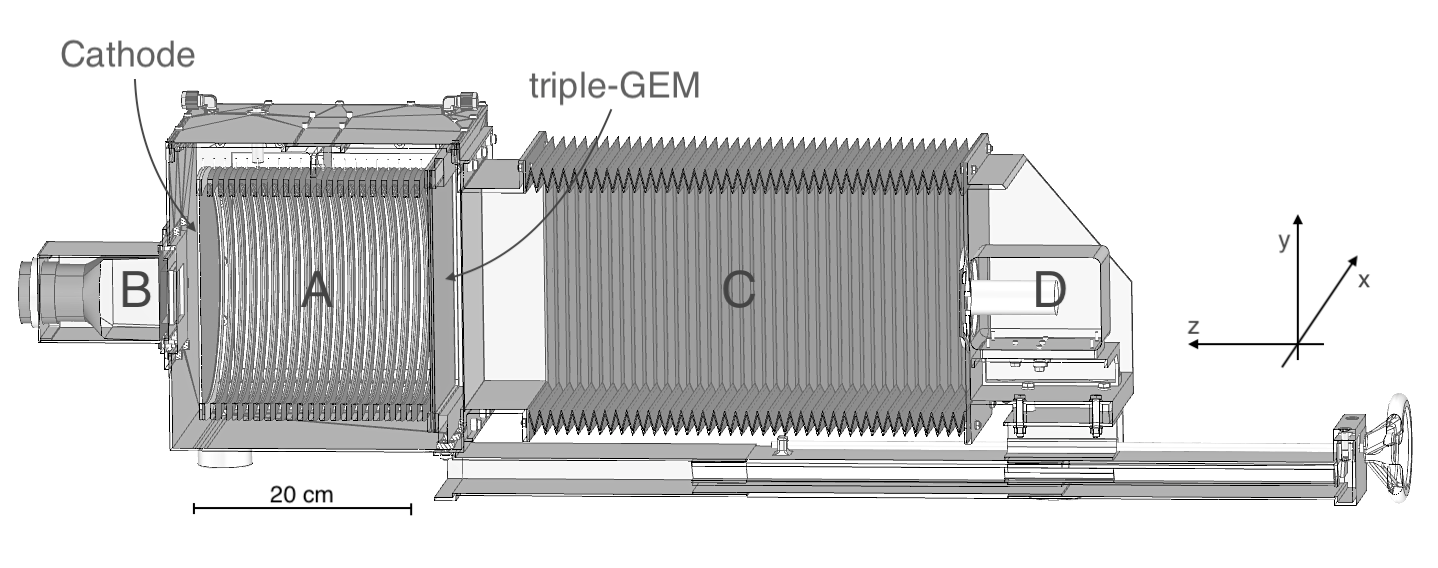
\includegraphics[width=0.70\linewidth]{figures/lemon.png}
        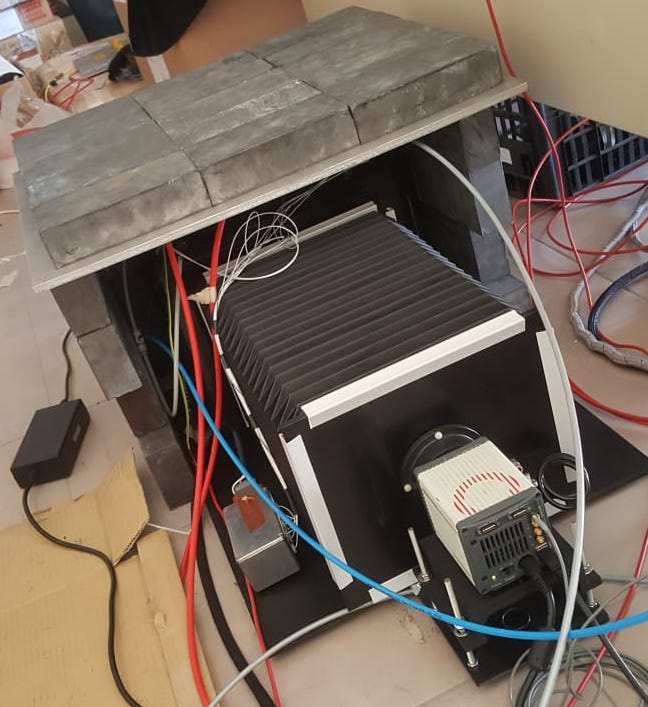
\includegraphics[width=0.20\linewidth]{LEMON-Shielded.jpg}
  	\caption{Left: the \lemon prototype with  its 7 liter sensitive
          volume (A), the PMT (B), the adjustable bellow (C) and the
          sCMOS camera with its lens (D). Right: \lemon
          with the lead shield around the drift volume cage. The sCMOS
          camera (on the front) is looking at the GEMs through a
          blackened bellow.
  	\label{fig:lemon}}
\end{figure}
%
The sensitive volume where the ionization electrons are drifting
 features a 200$\times$240\unit{mm$^2$} elliptical field cage
with a 200 mm distance between the anode and the cathode. The anode
side is instrumented with a 200$\times$240\unit{mm$^2$} rectangular
triple GEM structure.  Standard LHCb-like \cite{bib:thesis} GEMs
(70\unit{$\mu$m} diameter holes and 140\unit{$\mu$m} pitch) were used
with two 2\unit{mm} wide transfer gaps between them. The light emitted
from the GEMs is detected with an ORCA-Flash 4.0 camera
\cite{ORCAcamera} through a $203\times254\times1$\unit{mm$^3$}
transparent window and a bellow of adjustable length.  This camera
is positioned at a 52 cm distance from the outermost GEM layer and is
based on a sCMOS sensor with high granularity ($2048\times2048$
pixels), very low noise (around two photons per pixel), high
sensitivity (70\% quantum efficiency at 600\unit{nm}) and good
linearity. This camera is instrumented with a Schneider lens (with an
aperture f/0.95 and a focal length of 25\unit{mm}). The lens is placed
at a distance $d=50.6\unit{cm}$ from the last GEM in order to
obtain a de-magnification $\Delta = (d/f) - 1 = 19.25$ to image a
surface $25.6 \times 25.6$\unit{cm$^2$} onto the $1.33 \times
1.33$\unit{cm$^2$} sensor.  In this configuration, each pixel is
therefore imaging an effective area of 125$\times$125\unit{$\mu$m$^2$}
of the GEM layer. The fraction of the light collected by the lens is
evaluated \cite{bib:jinst_orange1} to be $1.7 \times 10^{-4}$.
%
A semi-transparent mesh was used as a cathode in order to collect
light on that side also with a 50$\times$50\unit{mm$^2$} \textit{HZC
  Photonics XP3392} photomultiplier \cite{PMTPhotonics} (PMT)
detecting light through a transparent $50\times50\times4$\unit{mm$^3$}
fused silica window. More details can be found in Ref.~\cite{paperBTF}.

A 5\unit{cm} thick lead shielding was mounted around the \lemon field
cage to reduce the environmental natural radioactivity
background. From the measurements of the GEM current with and without
the lead shielding, a factor two reduction in the total ionization
within the sensitive volume, very likely due to environmental
radioactivity, was estimated.


\section{Particle images  in \lemon gas volume}

The \lemon detector was operated in an overground location at
Laboratori Nazionali di Frascati (LNF) with a He-CF$_4$ (60/40) gas
mixture, the triple GEM system set at a voltage across the GEM sides
of 460\unit{V} and an electric field between the GEM layers of
2.5\unit{kV/cm}. A six independent HV channels \textit{CAEN A1257}
module
%a HV GEM power supply \cite{Corradi:2007df} 
ensured stability and monitored the bias currents with a precision
of 20\unit{nA}. The gas mixture was kept at atmospheric pressure under
continuous flow of about 200\unit{cc/min} and with the GEMs operated
at $2.0\times10^6$ gain. The typical photon yield
for this type of gas mixtures has been measured to be around 0.07
photons per avalanche electron\cite{bib:jinst_orange1, bib:roby,
  bib:tesinatalia}. The field cage was powered by a \textit{CAEN
  N1570}~\cite{CAENN1570}, generating an electric field of 0.5~kV/cm.
  
The motion of particles within the gas mixtures was studied by means
of different simulation tools. In particular,
\garfield~\cite{bib:garfield,bib:garfield1} program was used to
evaluate the transport properties for ionization electrons in the
sensitive volume for an electric field of 500\unit{V/cm}.

Given the diffusion in the gas, ionization electrons produced at a
distance $z$ from the GEM will distribute over a region on the GEM
surface, having a Gaussian transverse profile with a $\sigma$ given by:
%
\begin{equation}
\label{eq:diff}
\sigma = \sqrt{\sigma^2_0 \oplus D^2 \cdot z},
\end{equation}
where $D$ is the transverse diffusion coefficient,
calculated to be
%$D_{\mathrm{T}}^{60/40}~=~140~\frac{\mu{\mathrm{m}}}{\sqrt{\mathrm{cm}}}$.
$140~\mu{\mathrm{m}}/\sqrt{\mathrm{cm}}$.
The value of $\sigma^2_0$ was measured to be about
300\unit{$\mu$m} \cite{bib:btf,bib:fe55New}. Therefore, in average, a
point-like ionization will result in a spot of 3--4\unit{mm$^2$}.

The expected effective ranges of electron and He-nucleus recoils were
evaluated respectively with \GEANTfour~\cite{GEANT4} and with
\SRIM~\cite{bib:srim} simulation programs. The recoil range estimated
from simulation, as a function of the impinging particle kinetic
energy, is shown in Fig.~\ref{fig:range}. 
%
\begin{figure}[ht]
  \begin{center}
    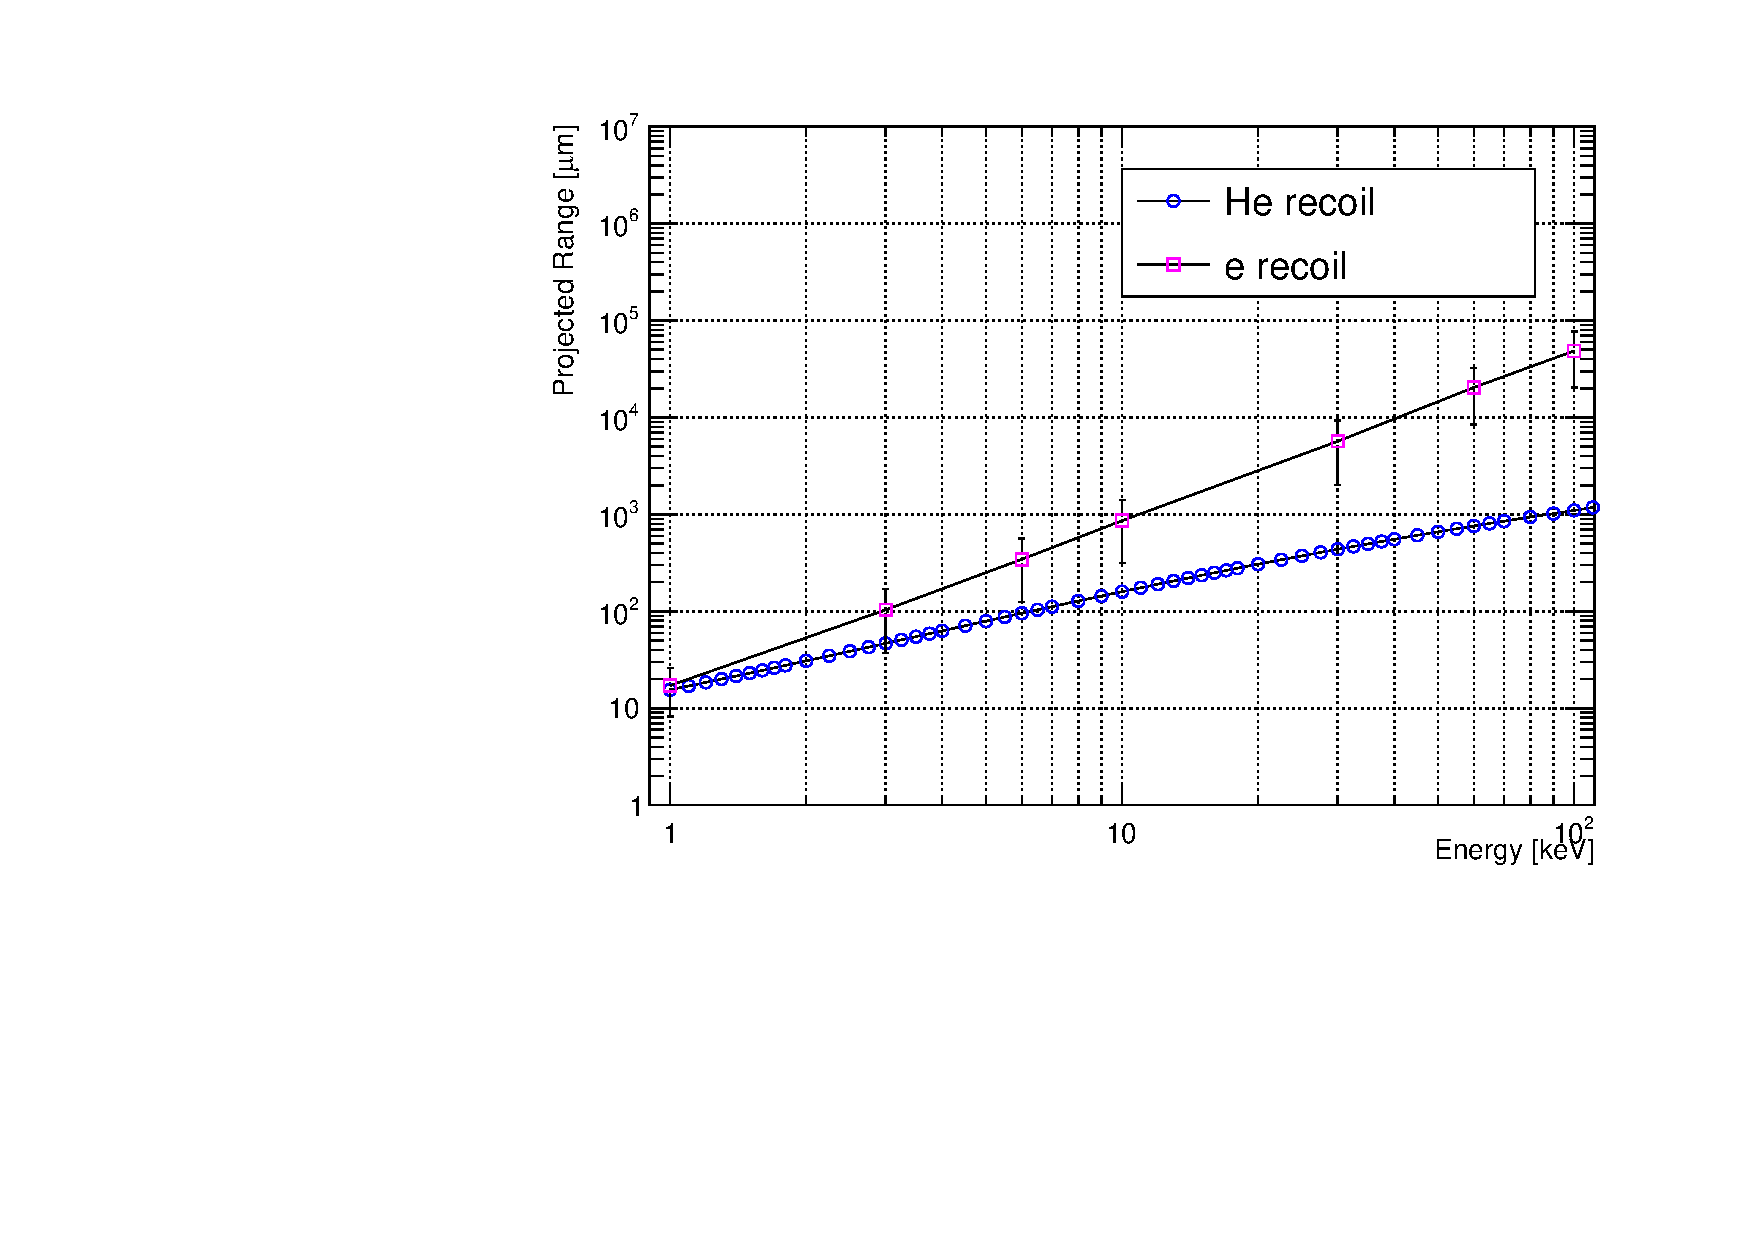
\includegraphics[width=0.49\linewidth]{figures/range_ER_NR.pdf}
    \caption{Average ranges for electron and He-nucleus recoils as a
      function of their kinetic energy.  \textcolor{red}{Range
        proiettato sulla direzione iniziale della traccia (parallela
        al piano delle GEM). Poco significativo. Spero che Giulia
        faccia un plot sul range 3D}
      \label{fig:range}}
      \end{center}
\end{figure}
%
These results show that:
\begin{itemize}
    \item He-nuclei recoils have a sub-millimetre range up to energies
      of 100\keV and are thus expected to produce bright spots with
      sizes mainly dominated by diffusion;
    \item low energy (less than 10\keV) electron recoils are in
      general longer than He-nucleus recoils with same energy and are
      expected to produce less intense spot-like signals. For a
      kinetic energy of 10\keV, the electron range becomes longer than
      1\unit{mm} and for few tens of \keV, tracks of few cm are
      expected.
\end{itemize}


The sCMOS sensor was operated in continuous mode with a global
exposure time of 30\unit{ms}. Typical images are shown in Fig.~\ref{fig:typicalimage1}. 

\begin{figure}[ht]
  \begin{center}
    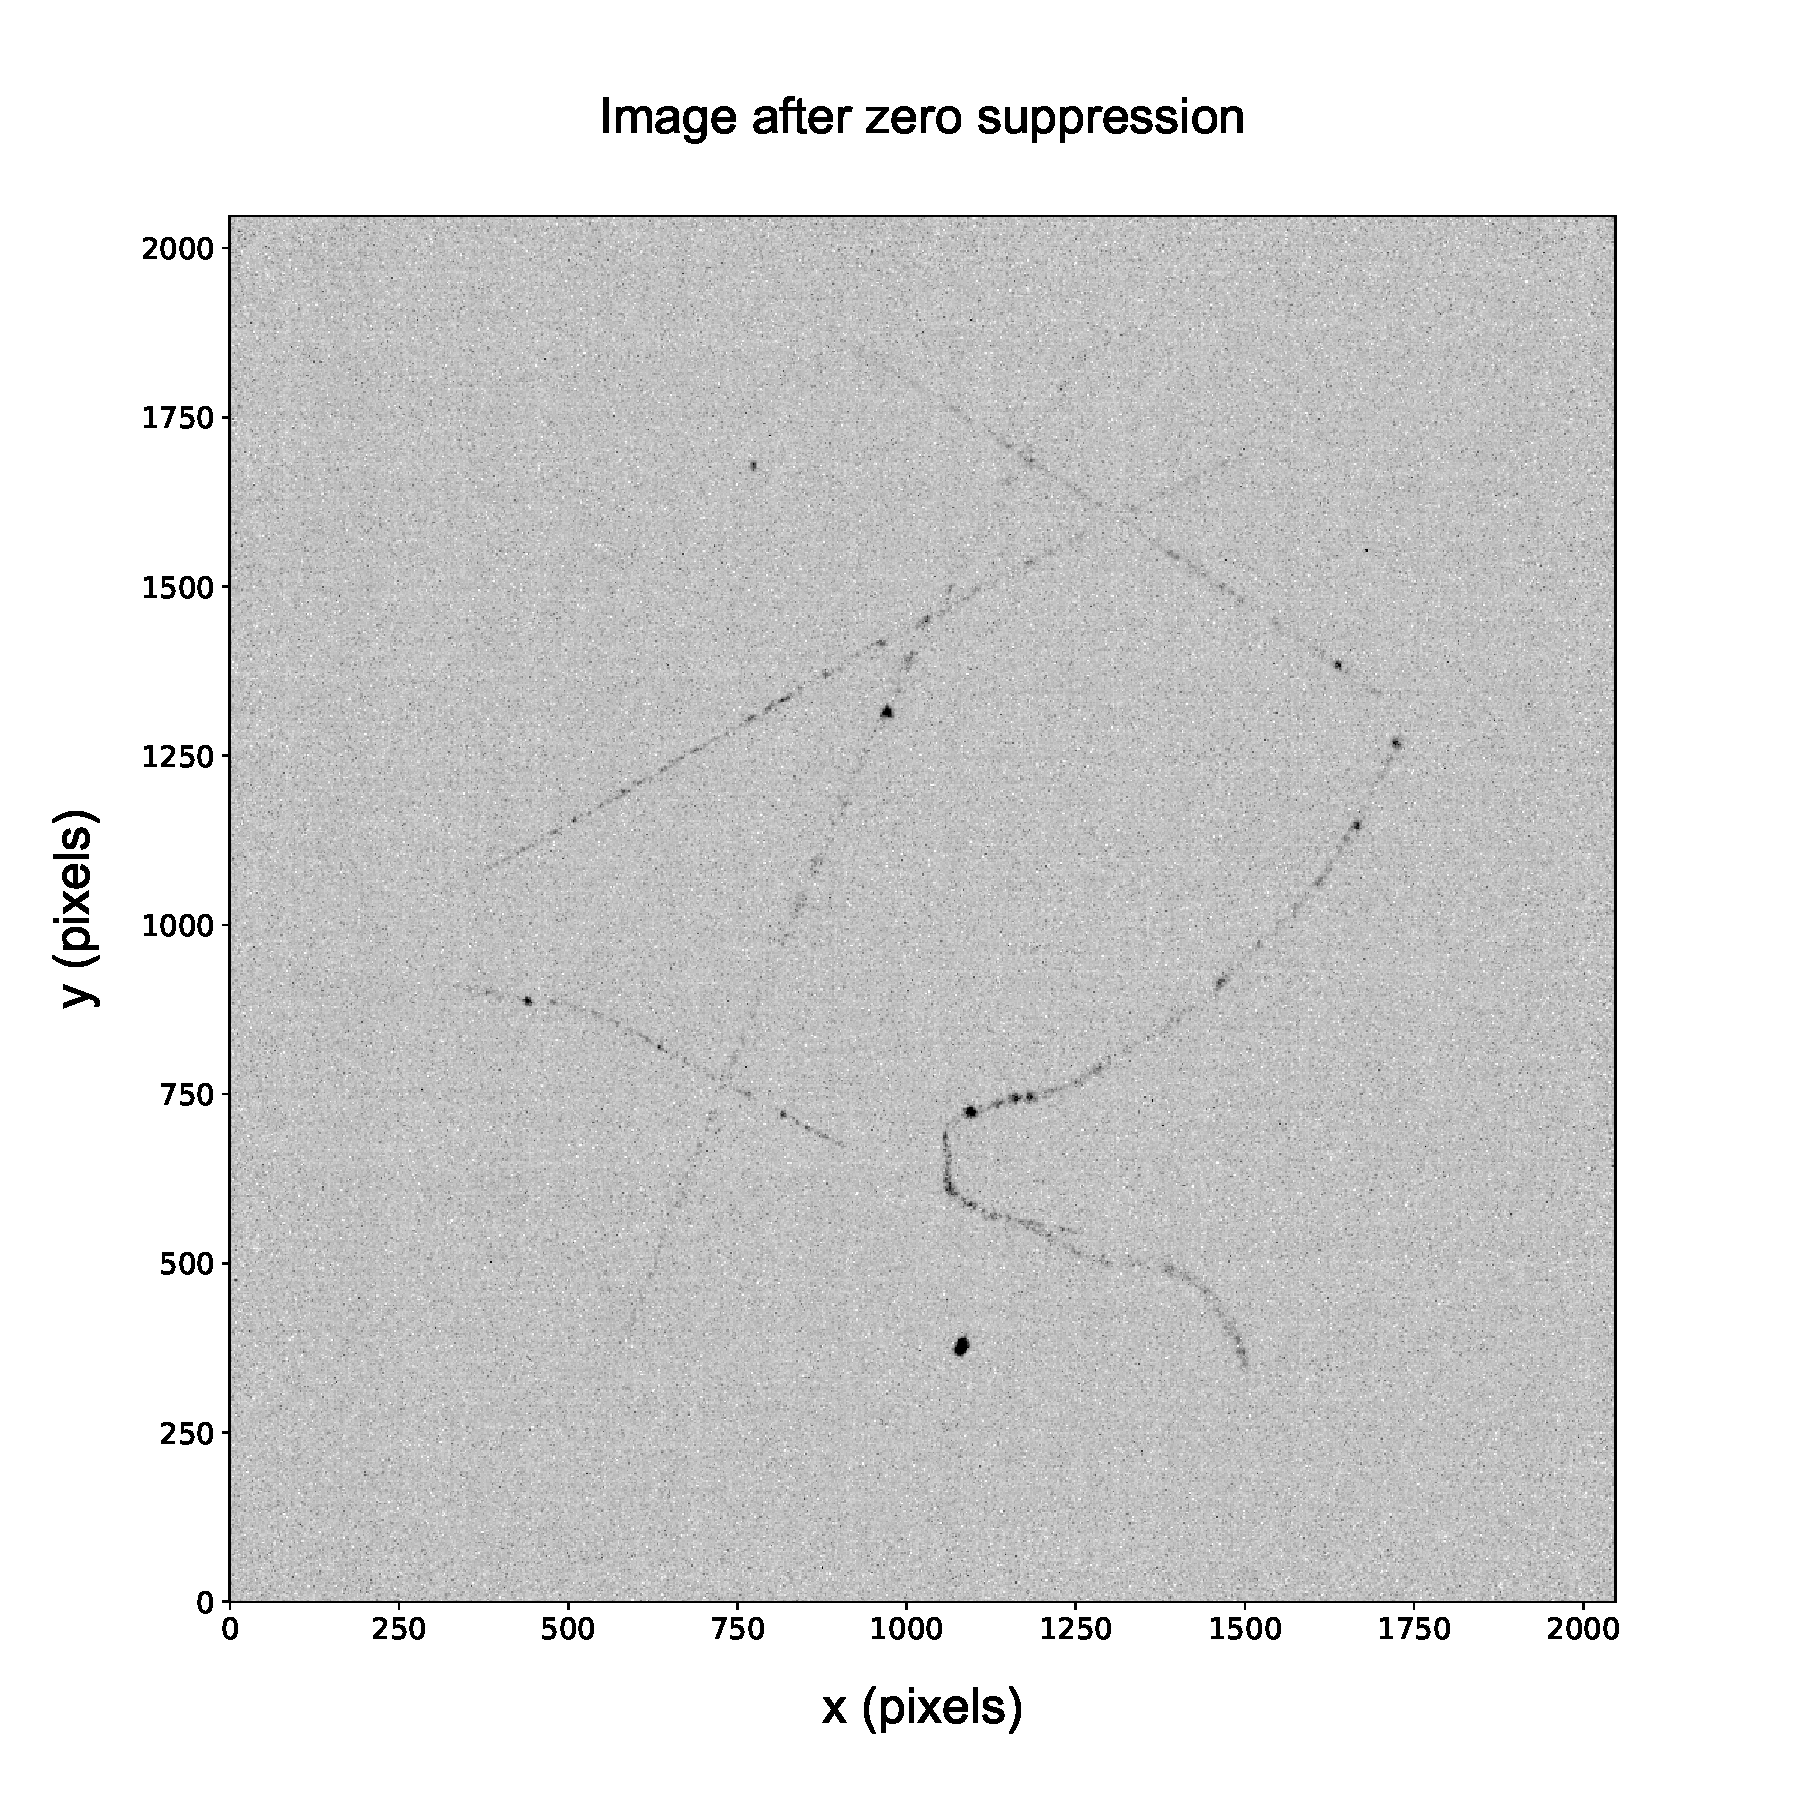
\includegraphics[width=0.49\linewidth]{figures/pic_run02317_ev8_oriIma_paper}
    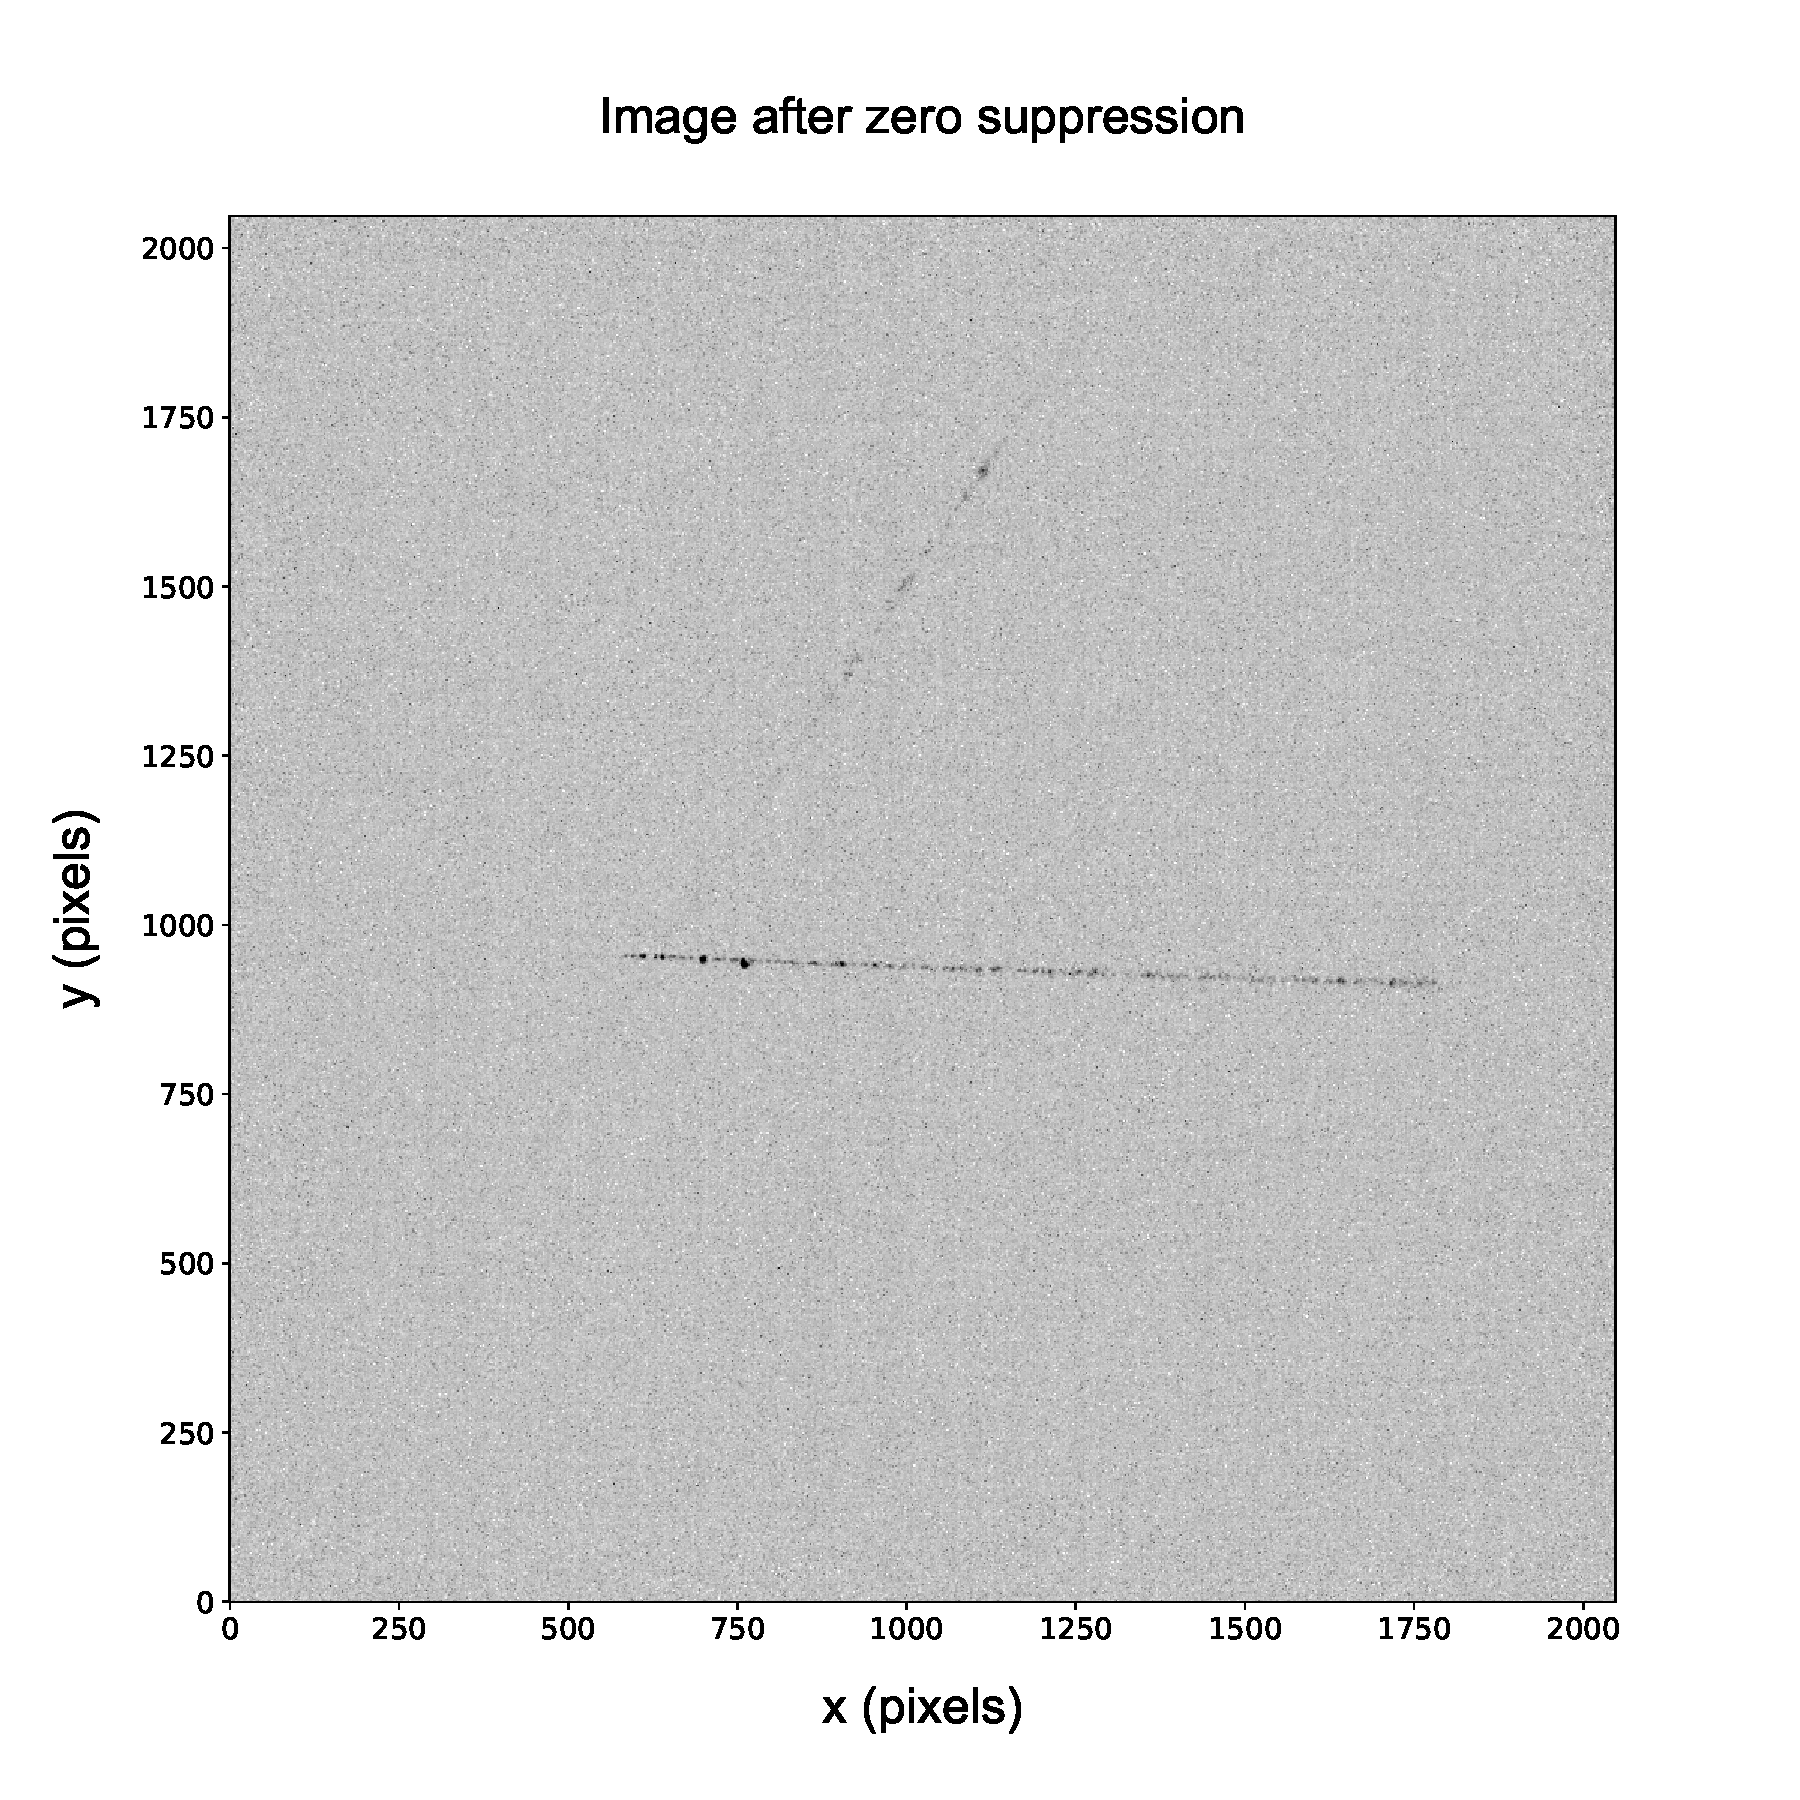
\includegraphics[width=0.49\linewidth]{figures/pic_run02156_ev527_oriIma_paper}
    \caption{Two typical pictures taken with the sCMOS camera with a
      30\unit{ms} exposure time. Left: cosmic tracks and natural
      radioactivity signals are present. Right: two long cosmic rays
      tracks are present, observed in a data taking run without any artificial source.
      \label{fig:typicalimage1}}
  \end{center}
\end{figure}

The PMT waveform was sent to a digitizer board with a sampling
frequency of 4\unit{GS/s}. The experiment trigger scheme is based on
the PMT signal: if, during the exposure time window, this exhibits a
peak exceeding a threshold of 80\unit{mV}, it is acquired in a time
window of 25\unit{$\mu$s} and the corresponding sCMOS image is stored.
The digitizer is operated in single-event mode. No more than one
signal is recorded in each sCMOS exposure time. Therefore, the PMT
information was mainly exploited to select events with a cosmic ray
track.
%% Forward reference is ugly. The picture is better later, when the difference Fe/cosm is explained.
%% Two examples of acquired waveforms are shown in
%% Fig.~\ref{fig:waveforms}.




Several light
spots are visible with different ionization patterns due to
different types of particles interacting in the gas.
Figure~\ref{fig:typicalimage1} (left) shows an image with typical long
tracks from cosmic rays traveling through the full gas volume, where
clusters of light with larger energy deposition are clearly visible,
superimposed to radioactivity events likely due to natural origin.
Figure~\ref{fig:typicalimage1} (right) shows an example of a cleaner
event with one straight cosmic ray track, that can be used for energy
calibration purposes.

Two different artificial radioactive sources were employed for testing and studying the detector responses.

\vspace{10pt}

A {\bf neutron} source, based on a $3.5\times10^3$\unit{MBq} activity
$^{241}$Am source contained in a Beryllium capsule (\ambe) was placed
at a distance of 50\unit{cm} from the sensitive volume side.  Because
of the interactions between $\alpha$ particles produced by the
$^{241}$Am and the Beryllium nuclei, the \ambe source isotropically
emits:
 \begin{itemize}
     \item photons with an energy of 59\keV produced by $^{241}$Am;
     \item neutrons with a kinetic energy mainly in a range 1--10\MeV
     \item photons with an energy of 4.4\MeV produced along with
       neutrons in the interaction between $\alpha$ and Be nucleus.
 \end{itemize}
 The presence of a lead shield around the sensitive volume absorbed
almost completely the 59\keV photon component. A small faction of them
reached the gas through small gaps accidentally present between the lead
bricks.

\vspace{10pt}

A \fe source emitting {\bf X-rays} with a main energy peak at 5.9\keV.
This is the standard candle for calibration and performance evaluation
of \lemon, and its extensive use is documented in
Ref.~\cite{bib:fe55}.

\vspace{10pt}

The events in Fig.~\ref{fig:signals} show images recorded with the
same 30~ms exposure time, in presence of the two sources. The left
panel shows an example of several light spots, characteristic of
energy deposits due to \fe low energy photons.  The right panel shows
a frame recorded in presence of the \ambe radioactive source: the
short and bright track well visible in the center is very likely
due to a nuclear recoil induced by a neutron scattering.
% 
\begin{figure}[ht]
  \begin{center}
    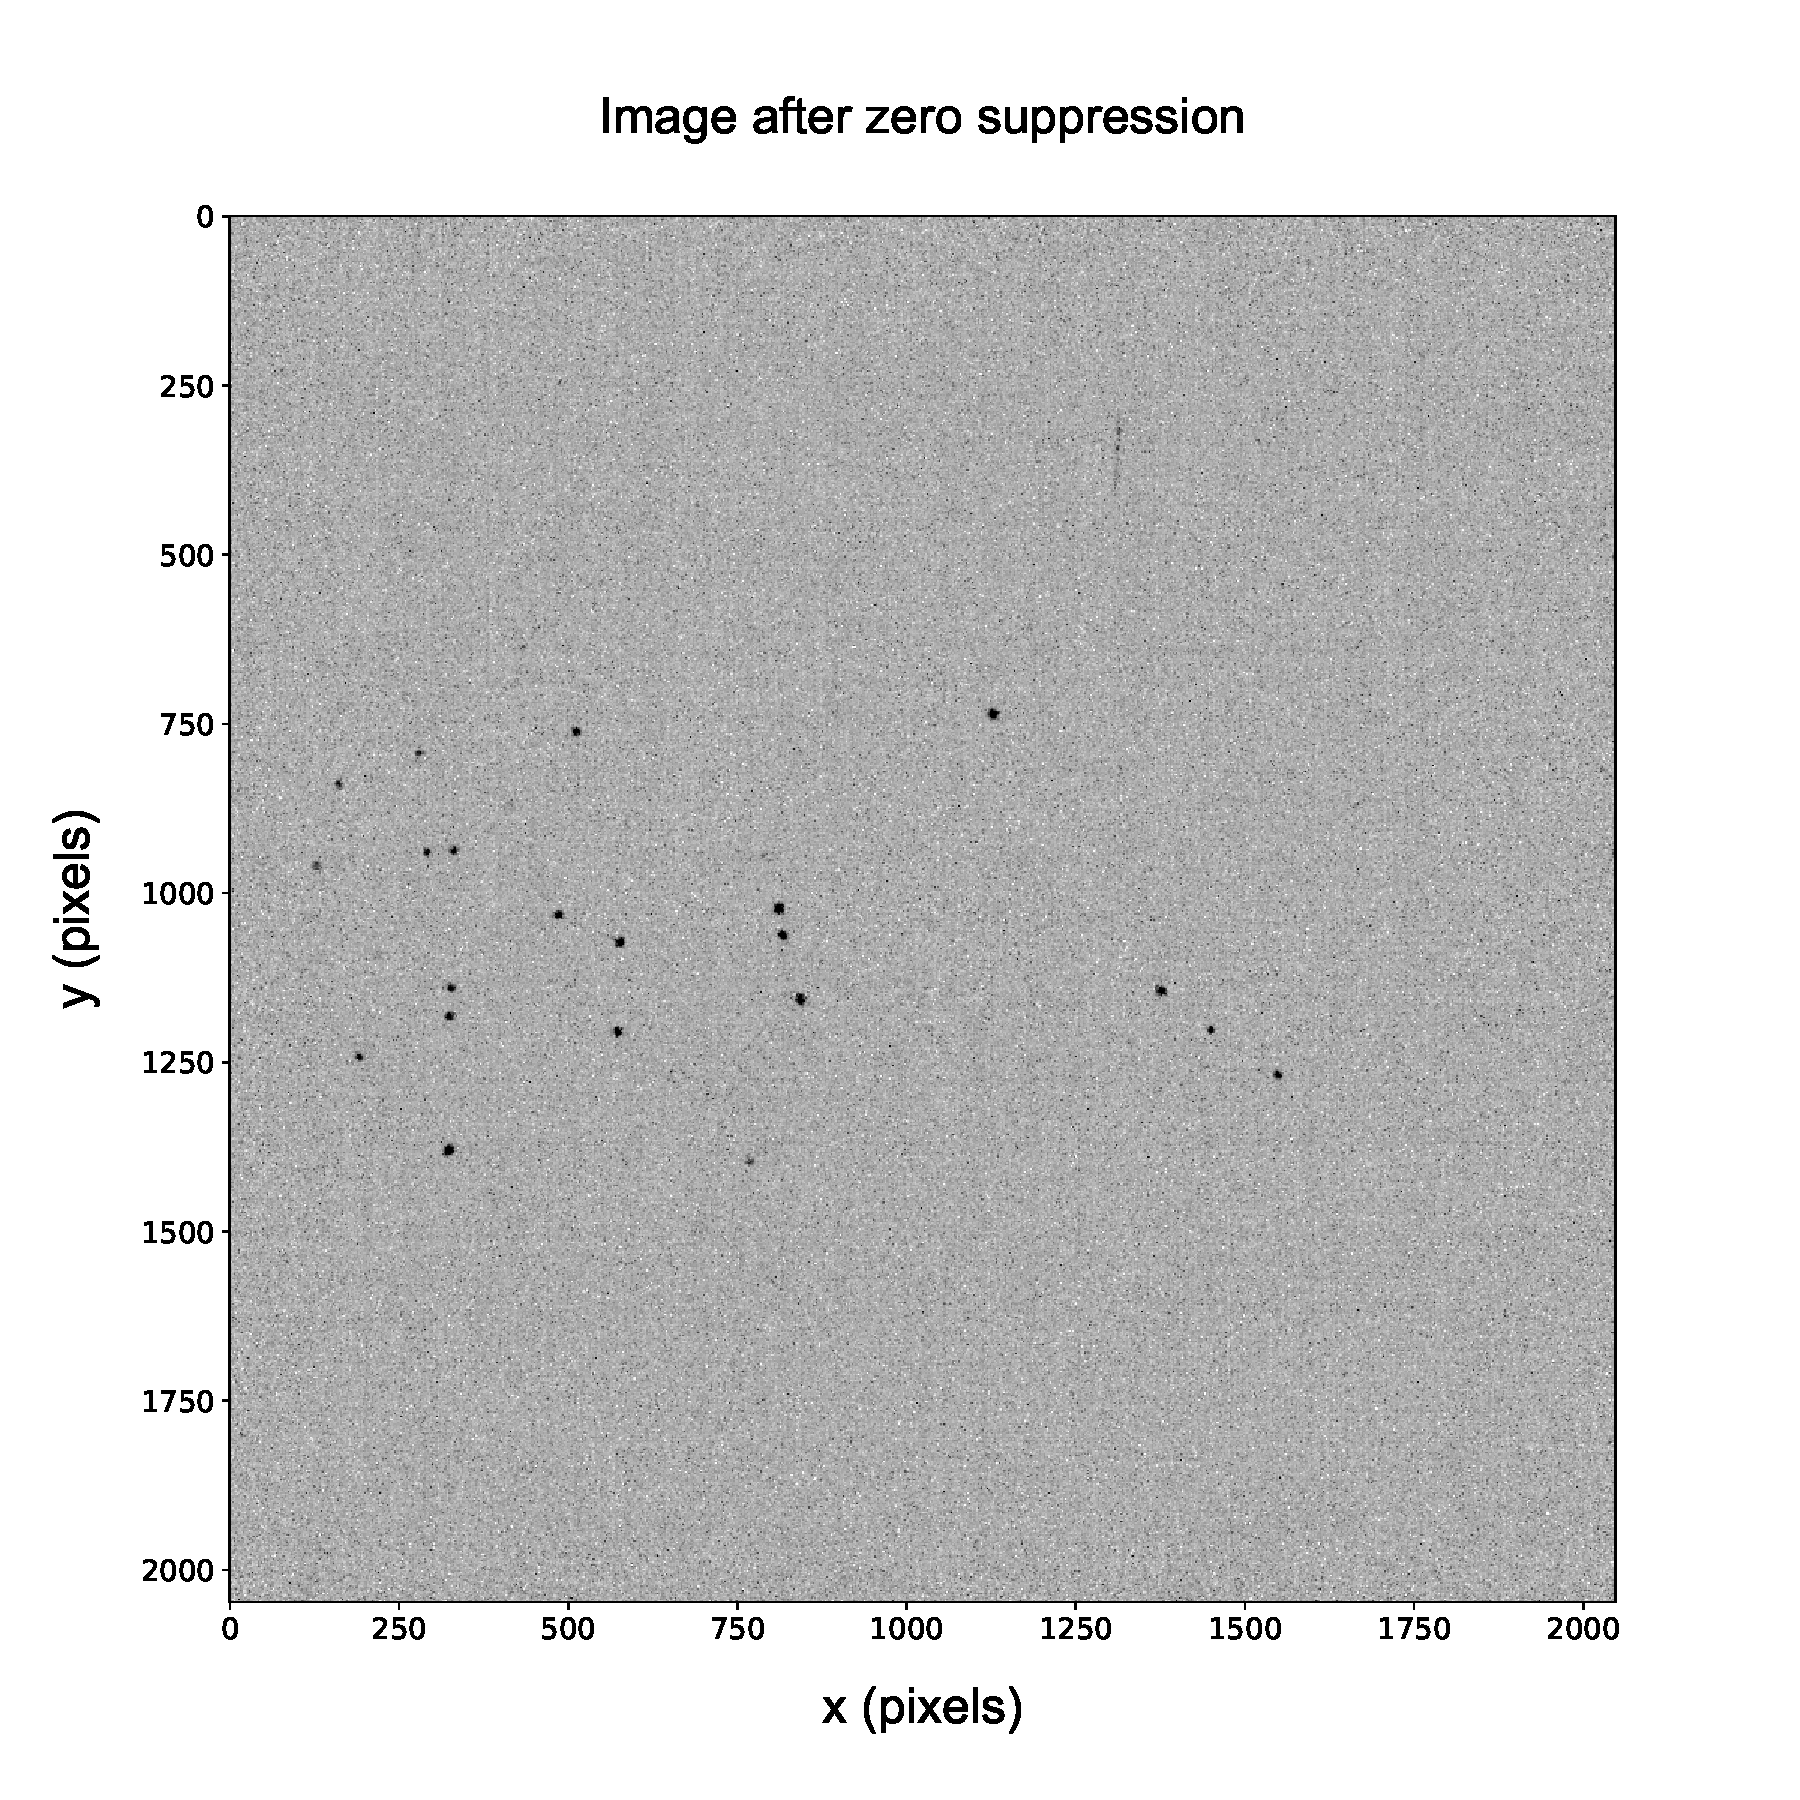
\includegraphics[width=0.49\linewidth]{figures/pic_run01843_ev93_oriIma_paper}
    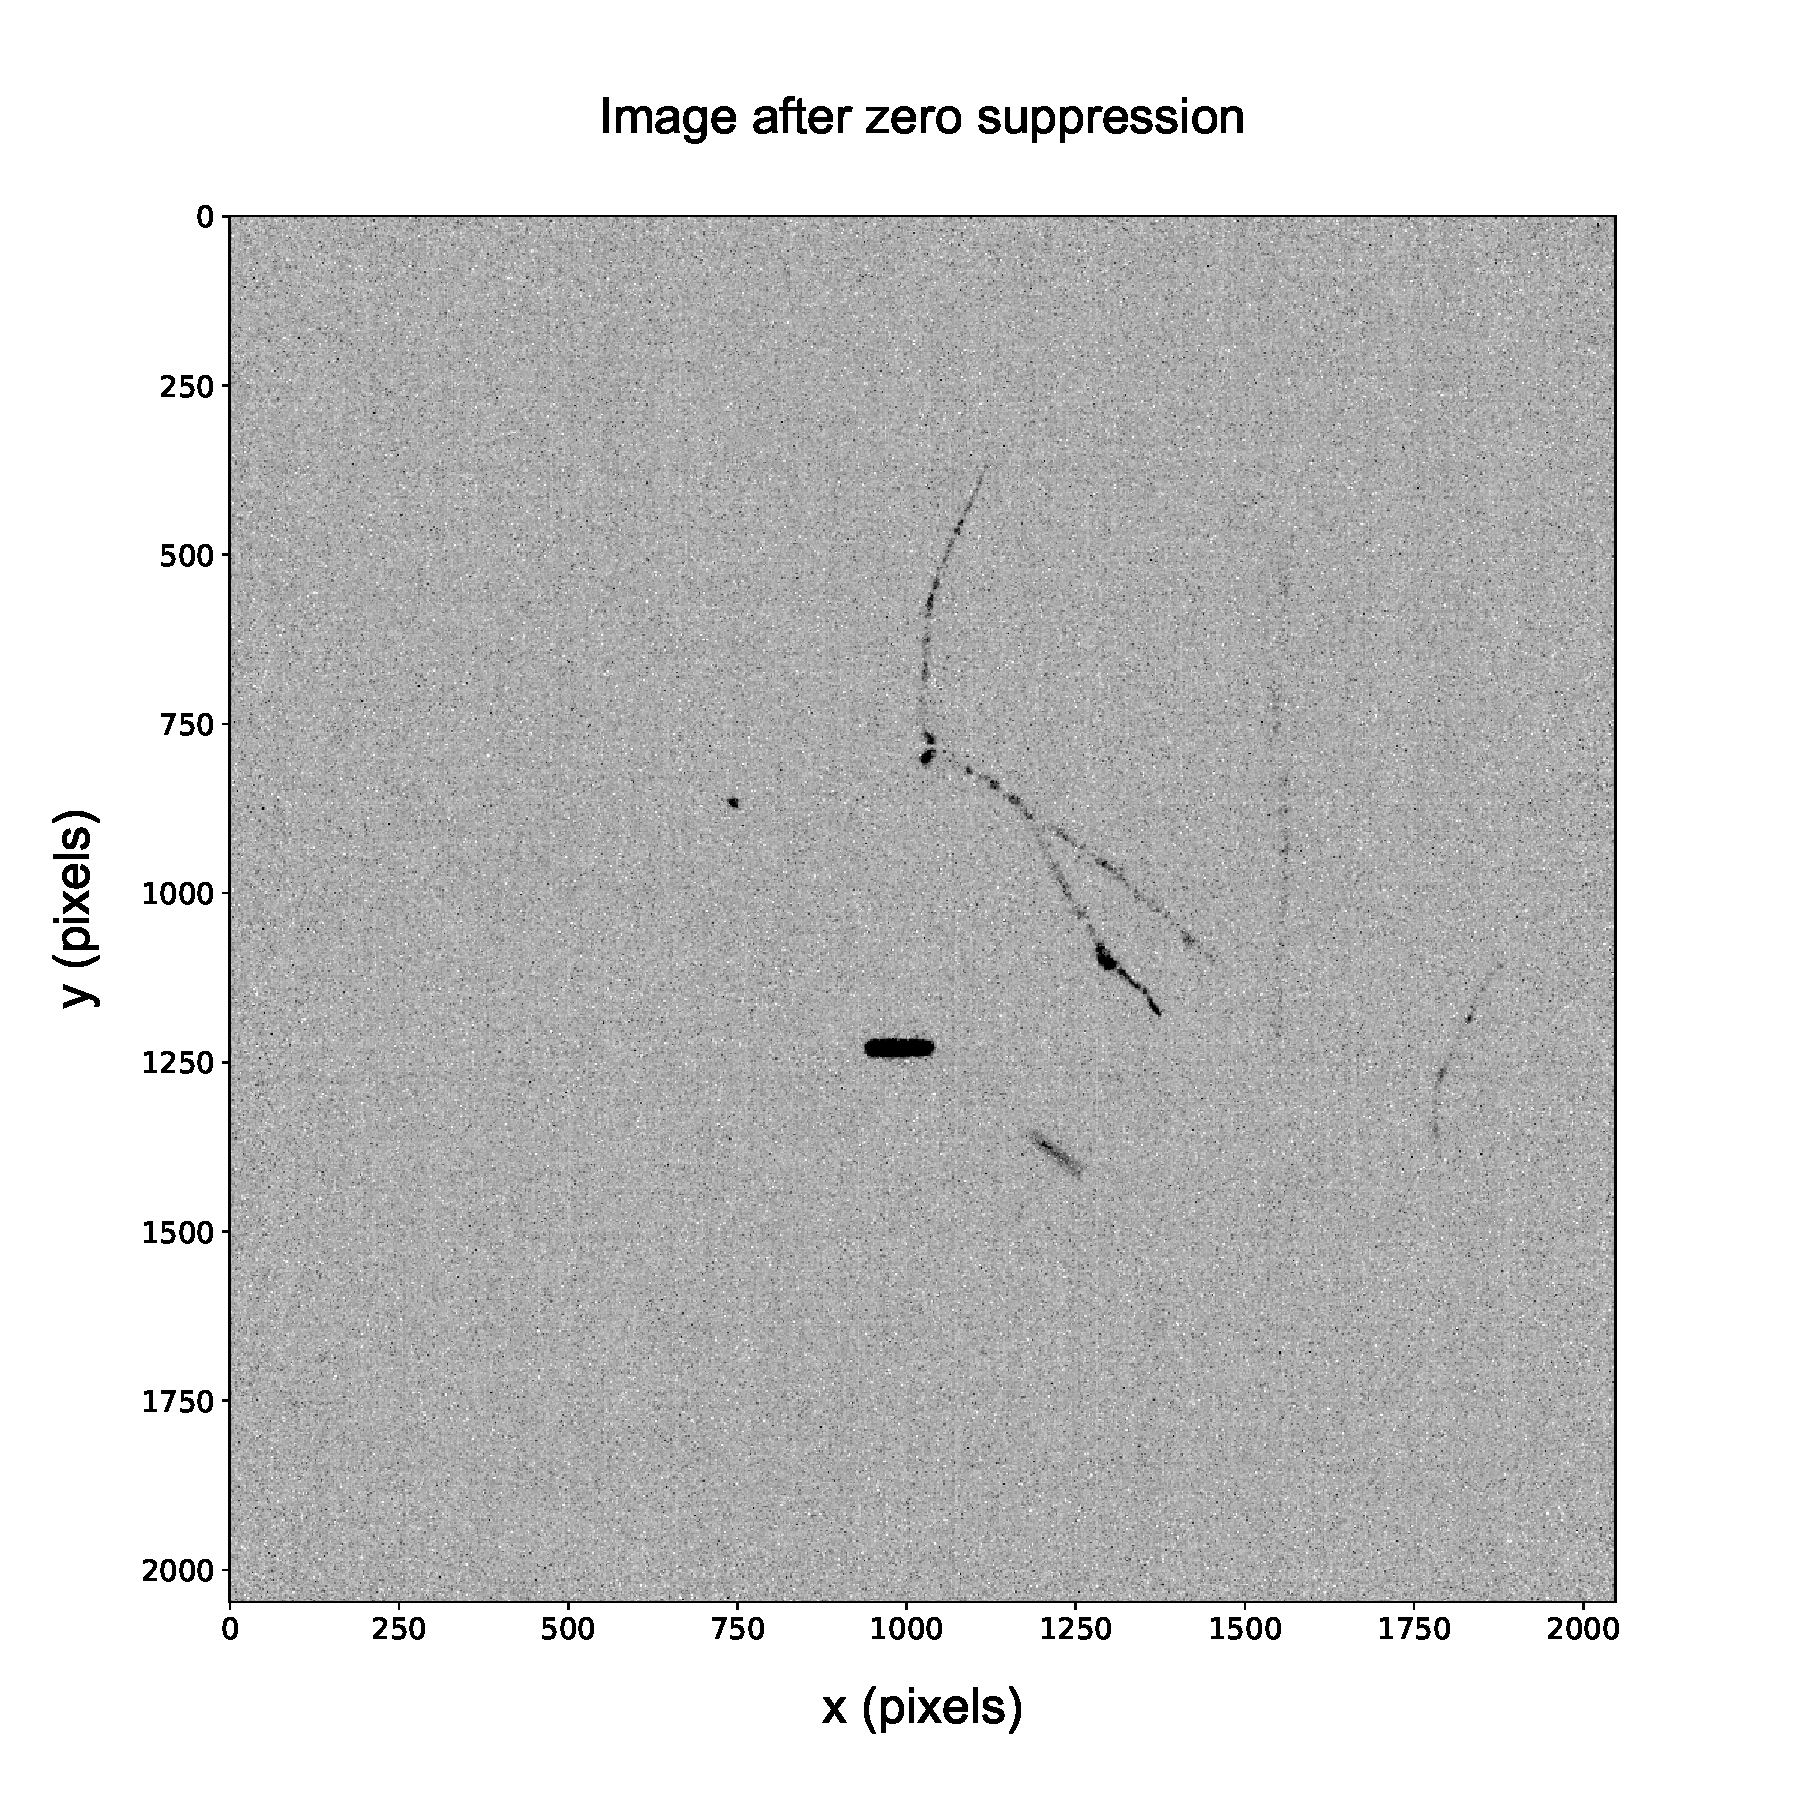
\includegraphics[width=0.49\linewidth]{figures/pic_run02317_ev342_oriIma_paper}
    \caption{Two pictures taken with the sCMOS camera with a 30 ms
      exposure time. Left: picture taken in presence of \fe radioactive
      source. Right: a nuclear recoil candidate is present, in an image
      with \ambe radioactive source, together with signals from natural
      radioactivity.      \label{fig:signals}}
  \end{center}
\end{figure}




\clearpage
 
\section{Cluster pattern recognition}
\label{sec:clustering}
The light produced in the multiplication process in the GEM and
detected by the sCMOS sensor is associated in clusters of neighboring
pixels. This is done by following the trail of energy deposition of
the particle traveling through the gas of the sensitive volume. The
deposited energy (that for stopped particles is equivalent to the
total energy of the particle) is estimated by the amount of the light
collected by the sensor.  Therefore, it is of primary importance to
have a reconstruction algorithm that includes all the camera pixels hit by
the real photons originating from the energy deposits, while rejecting
most of the electronic noise. This can either create fake clusters or,
more likely, add pixels in the periphery of clusters of real
photons, biasing the energy estimate.

The energy reconstruction follows a three-steps procedure: the
single-pixel noise suppression is briefly described in
Section~\ref{sec:zerosuppression}. This is followed by the proper
clustering: first the algorithm to form basic clusters from single
small deposits is described in Section~\ref{sec:basiccl}, then the
supercluster method, aiming to follow the full track pattern, and
seeded by the basic clusters, is described in
Section~\ref{sec:supercl}.

The results of this paper are based on the properties of the
reconstructed superclusters and are described in
Section~\ref{sec:clustershapes}.


\subsection{Noise suppression}
\label{sec:zerosuppression}
The electronic noise of the sensor was estimated in data-taking runs acquired with
the sensor in complete dark ({\it pedestal} runs). For each pixel, the
pedestal was computed as the average of the counts over many frames,
while the electronic noise was estimated as their standard deviation
(SD). The distribution of the pixels SD is shown in
Fig.~\ref{fig:noise}. The mode of this distribution is about 1.8
photons per pixels, but a tail is present, with pixels having a noise
of more than 5 photons per pixels. For such pixels, a very
non-Gaussian distribution was observed, while for the pixels in the
bulk of the distribution, the pedestal distribution followed a Gaussian
shape. To form the pedestal-subtracted image, the pedestal mean
$\mu_i$ was subtracted to the image for each $i^{th}$ pixel.  An initial
noise suppression was applied by neglecting the pixels with counts less
than $1.3\times\textrm{SD}_i$.
%where $i$ represents the
%pixel (\textit{zero suppression}). 
%
\begin{figure}[ht]
  \centering
  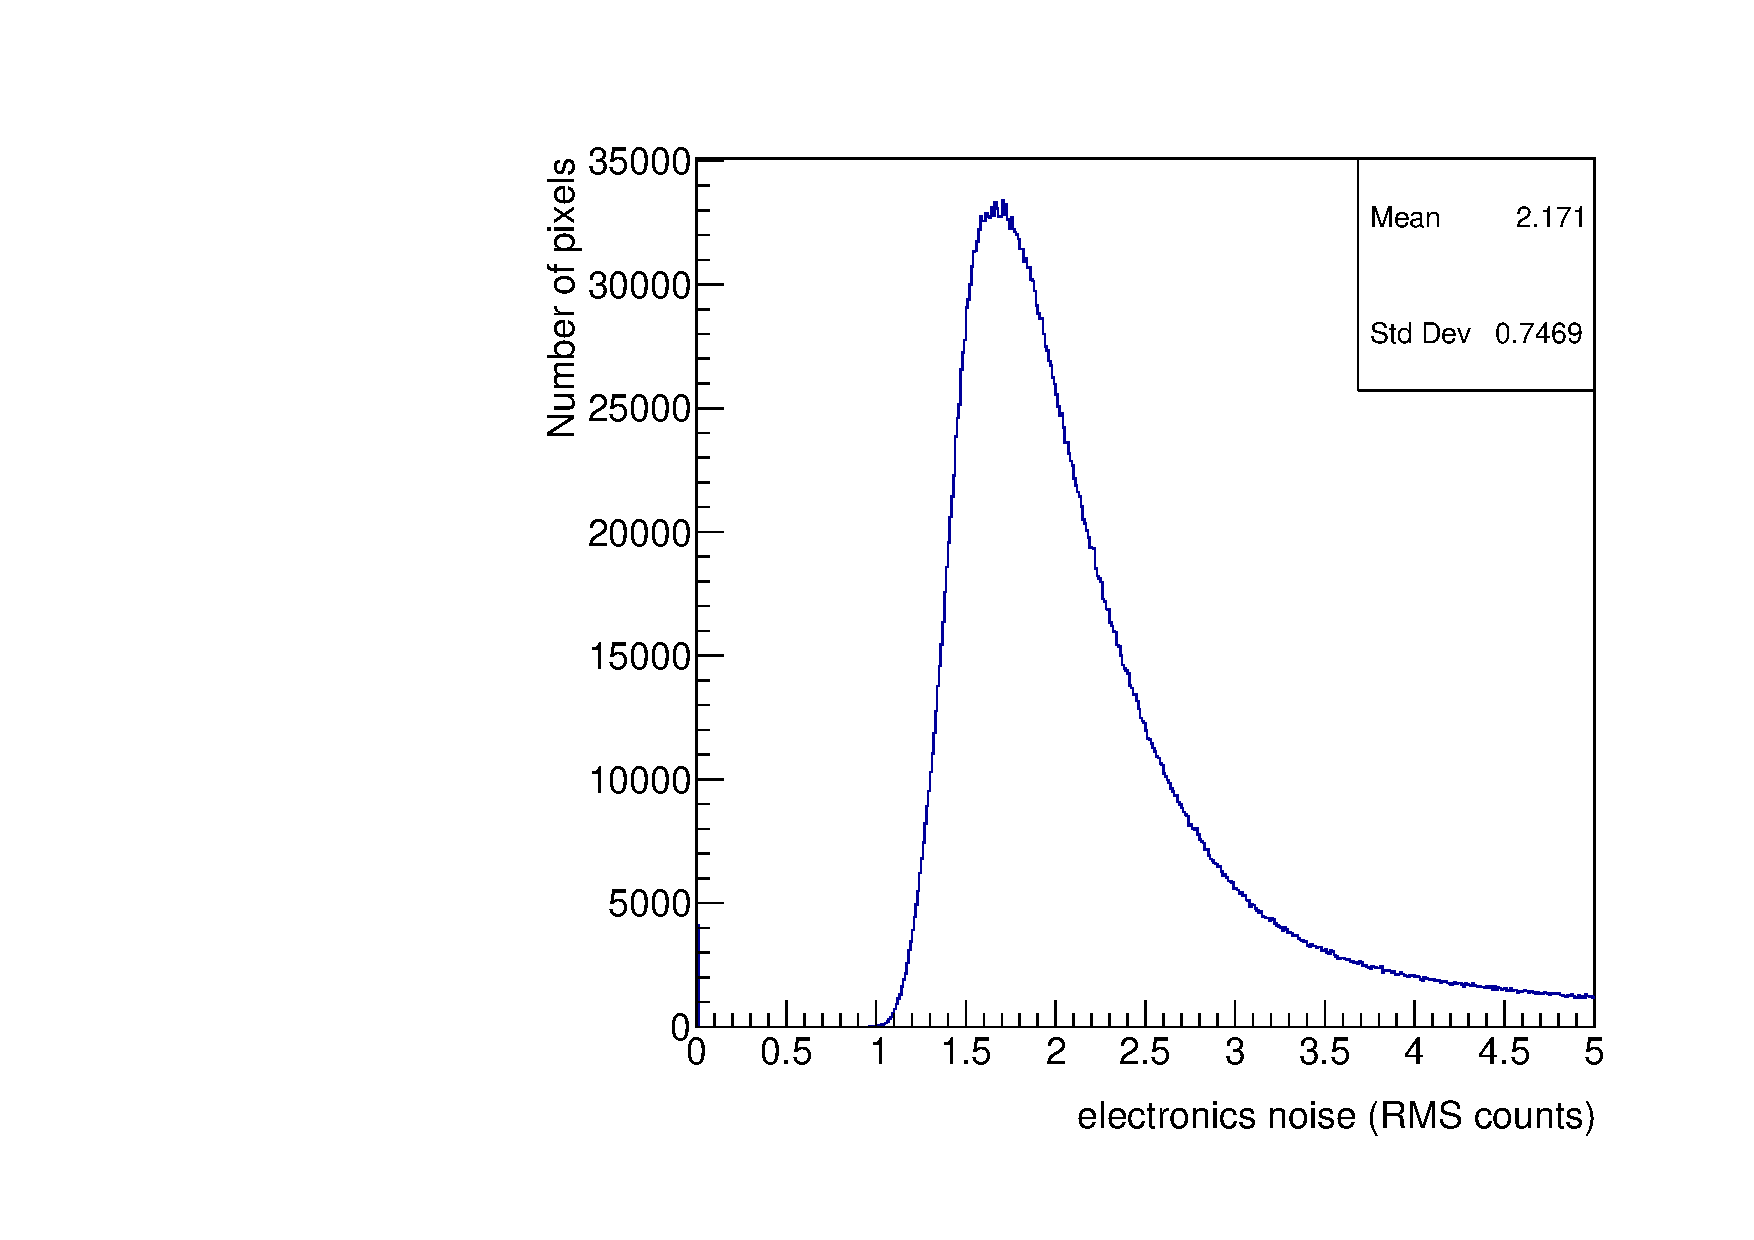
\includegraphics[width=0.45\linewidth]{figures/sensor_noise}
  \caption{Distribution of the electronic noise of the sensor,
    estimated in images taken with sensor in complete dark, and
    evaluated as the SD of the distribution of the counts for each
    pixel.  \label{fig:noise}}
\end{figure}
%
On such pedestal-subtracted zero-suppressed images an upper threshold
was applied to reject hot pixels, which are more likely due to sensor
instabilities than to energy deposition. These were found  to be not
malfunctioning pixels since they disappeared after a power cycle of the
camera: therefore a dynamic (run-by-run) suppression was needed.
They were efficiently identified as high-intensity, isolated pixels,
and distinguished by a true energy deposit, for which each pixel is
surrounded by some other active pixels. A threshold was applied on the
ratio $R_9$ between the pixel and the average of the counts in a
$3\times3$ pixels matrix surrounding it, and a minimum number of two
pixels above noise in that matrix was required to discriminate  good from
hot pixels.

The resolution of the resulting image was then reduced by forming
\textit{macro-pixels}, by averaging the counts in $4\times4$ pixel
matrices. This was needed to reduce the combinatorics   of the subsequent
clustering algorithm to be executed   in a reasonable time for each
image. On such $512\times512$ pixel map, a median
filtering~\cite{medianfilter} was applied, as described in more details
in Ref.~\cite{medianfilter_cygno}. The output image is passed to the
basic clustering algorithm, described in the following.





\subsection{Basic clusters reconstruction}
\label{sec:basiccl}
The basic clustering algorithm, called \idbscan and described in
details in Ref.~\cite{iDBSCAN}, represents an improvement of the
neighboring pixels clusters, called \nnc, previously used to study the
performance of the \lemon detector with \fe radioactive
source~\cite{bib:fe55}. It is briefly described also here, since it
represents the seeding for the final clustering algorithm.

The energy deposition in the sensitive volume of the TPC is estimated
from the two-dimensional (2D) projection on the $x$--$y$ axes of the
light emitted in the multiplication process within the GEMs
planes. The pattern shows a large variation, depending on the
interacting particle. For images recorded with the \fe calibration
source, the signature of the typical 5.9\keV photons is a spot of few
mm$^2$, with the exact size depending on the diffusion in the
gas, \ie, on the distance from the anode, along $z$, of the point
where the energy release happens (see Fig.~\ref{fig:signals}
left). Muons from cosmic rays travel across the gas volume and leave a
typical signature of a straight track, shown in
Fig.~\ref{fig:typicalimage1} (right), but with several agglomeration
with larger density along the path. Natural radioactivity shows an
irregular pattern, sometimes curly, with several kinks along the
path. Finally, the signal from nuclear recoils due to neutrons,
originated by the \ambe source, is expected to be spot-like, or to
emerge as short straight tracks with a length smaller than 1\unit{mm}
for energies below 100\keV, as shown by Fig.~\ref{fig:range}.

Their track length and their size is found to depend a lot on the
initial energy of the impinging neutron, and also on the mass of the
recoiling nucleus in the He-CF$_4$ gas mixture utilized in
the \lemon detector.

Thus, the clustering algorithm needs to be flexible enough to
efficiently reconstruct a diverse set of patterns, from small round
spots to long and kinky tracks. A first step of the clustering,
called \textit{seeding}, is used: it focuses in the clustering of
spot-like neighboring pixels.  The method applied for the \lemon
detector is an evolution of the classic \dbscan
algorithm~\cite{dbscan}.  This is a non-parametric, density-based
clustering, which groups together pixels above threshold with many
neighbors, within a circle with a radius $\epsilon$. Its distinctive
characteristics making this method very suitable to the \lemon case is
its ability to label as outliers, and so not to include in the
clusters, pixels that lie isolated in low-density regions, \ie, pixels
from electronic noise of the sensor surviving the zero
suppression. The extension of \dbscan used for \lemon data analysis
consists in including a third dimension to the phase space of the
points considered, adding to the pixel position ($x$--$y$ coordinates)
the measured number of photons in that pixel, $N_{ph}$.  This approach
improves the combinatorial background rejection and the energy
resolution with respect the previously used \nnc algorithm, as
described in details in Ref.~\cite{iDBSCAN}.

To be as inclusive as possible, and since different interactions may
have vastly different intensities, even varying along the track, the
clustering procedure is iterated three times.  First, the \dbscan
parameters were tuned to form clusters of dense (in $x$--$y$ dimension)
and intense (in the $N_{ph}$ dimension) pixels. The density in 3D is
called \textit{sparsity}.  This step typically identifies either rare
hot spots of the GEMs, or, efficiently, short nuclear recoils. The
pixels belonging to the reconstructed clusters are then removed from
the image, and the \dbscan procedure is repeated, with looser sparsity
parameters. The second iteration is tuned to efficiently reconstruct
\fe round spots and slices of tracks from nuclear recoils with lower
intensity. It also collects the agglomeration with larger density
along cosmic tracks, clearly visible in the example in
Fig.~\ref{fig:typicalimage1} (right).  A third iteration of \dbscan
with even looser parameters is finally executed, targeting faint
portions of a cluster. These are especially used as a proxy for the
characterization of clustered noisy pixels, while the first two are
used as seeds for the final clustering step, described in
Sec.~\ref{sec:supercl}.

To be computationally viable, the \idbscan basic clustering is
performed on the image with reduced resolution, 512$\times$512. In
typical images this allows the basic clusters reconstruction to be run
in approximately 1\unit{s} on an \texttt{Intel Xeon
E5-2620}~2.00\unit{GHz} and 64\unit{GB} RAM. The reconstruction
algorithm is implemented in \PYTHONthree~\cite{python3}, and
interfaced with the CERN \ROOT v.6~\cite{root}.


Examples of clustered pixels in two cases are shown in
Fig.~\ref{fig:basic_clusters}. The left panel shows an example of
clusters reconstructed on the low-resolution image of one event
with \fe source. Three spots are clearly visible: one, as typical for
events with this calibration source with a moderate activity, is
reconstructed by a single cluster of the second iteration. The other
two are close enough that are merged in a single cluster of the same
iteration. The cases of merged spots containing twice the energy of a
single X-ray deposit, given the activity of the \fe source, represent
about one tenth of the clusters in this set of runs. The energy
resolution is good enough to distinguish statistically the single and
merged spots, as will be described in Sec.~\ref{sec:calibration}.  The
optimization of the \idbscan parameters is done assuming a low pileup
of events, typical of the running conditions for a future underground
run of the \cygno project, of which \lemon is the prototype, where the
occurrences of such cases are expected to be negligible.

The right panel shows the outcome of the \idbscan algorithm on a
longer track, presumably from natural radioactivity, and one possible
short nuclear recoil.  The nuclear recoil candidate is very dense,
highly-energetic, and isolated. Therefore, it is reconstructed as a
single cluster in the first iteration. The long track shows several
clusters with higher intensity. One of them has a large energy, and it
is reconstructed as an isolated single iteration-1 cluster. The rest
of the track is reconstructed by multiple iteration-2 clusters, which
are split where the energy deposition has a minimum extending across
too many pixels to be joined together in the same cluster. Events like
these, which are frequent for muons, natural radioactivity, but also
signals from $\alpha$-particles with higher energy, originating by the
possible interaction of neutrons with the plastic material of the
field cage, justify the need of the subsequent step of
the \textit{superclustering}, which follows the track without
splitting it in parts. This is described in the following section.
%
\begin{figure}[ht]
  \begin{center}
     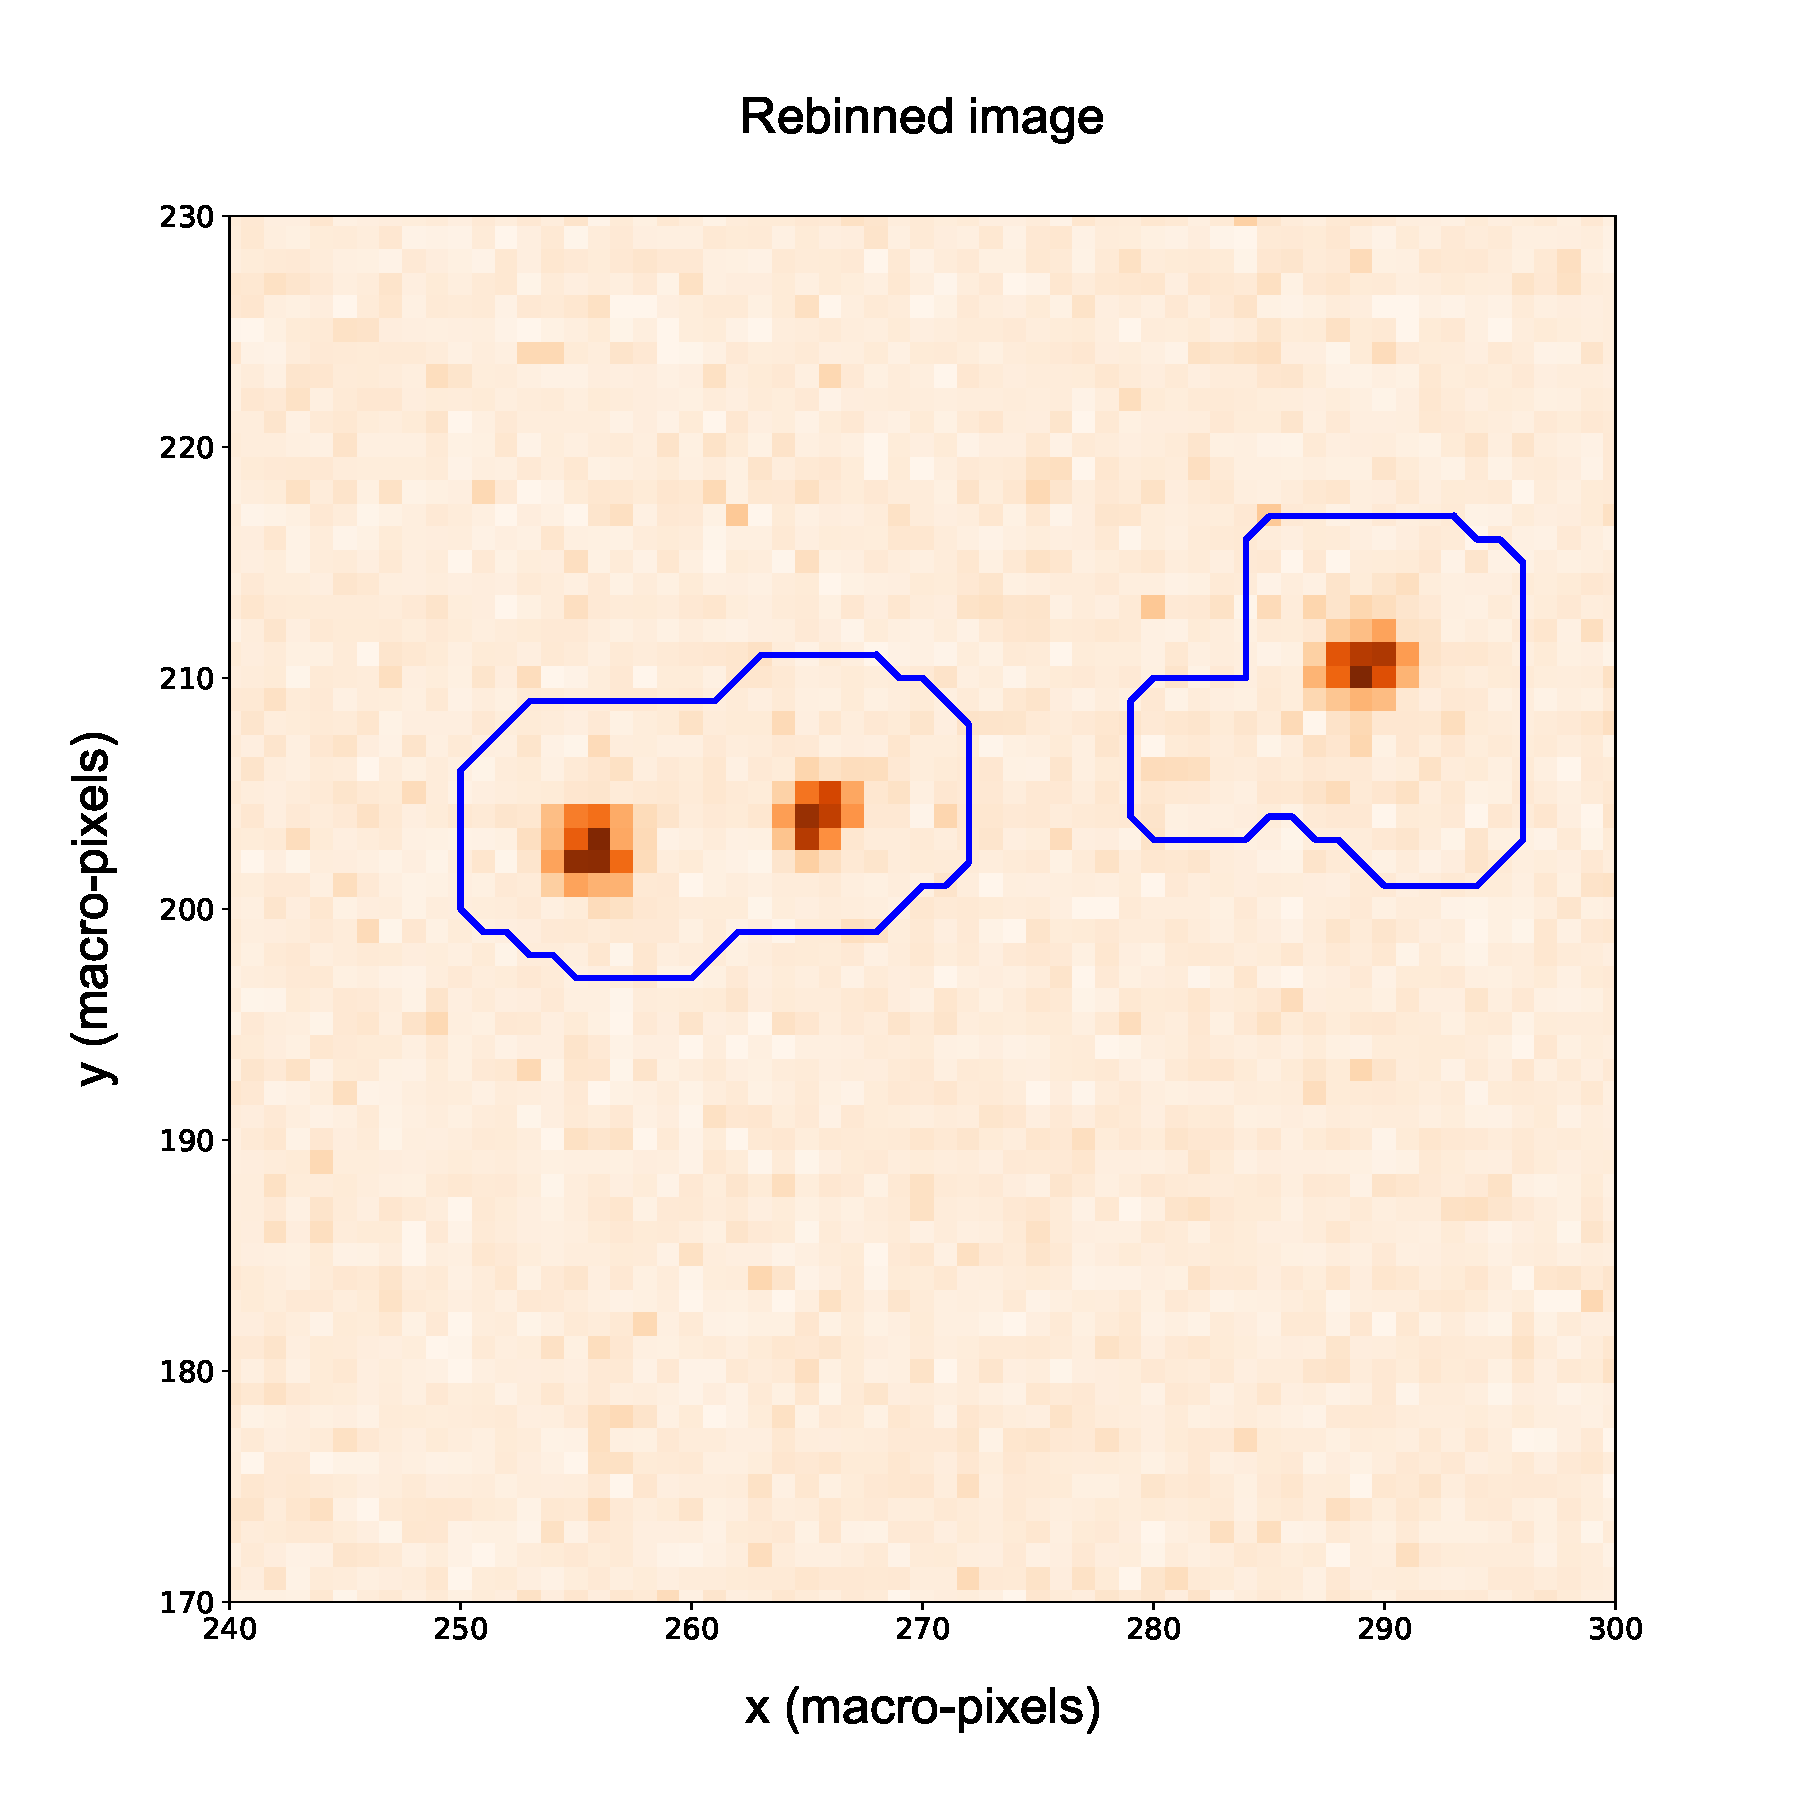
\includegraphics[width=0.49\linewidth]{figures/pic_run01843_ev93_2nd_3D_paper}
      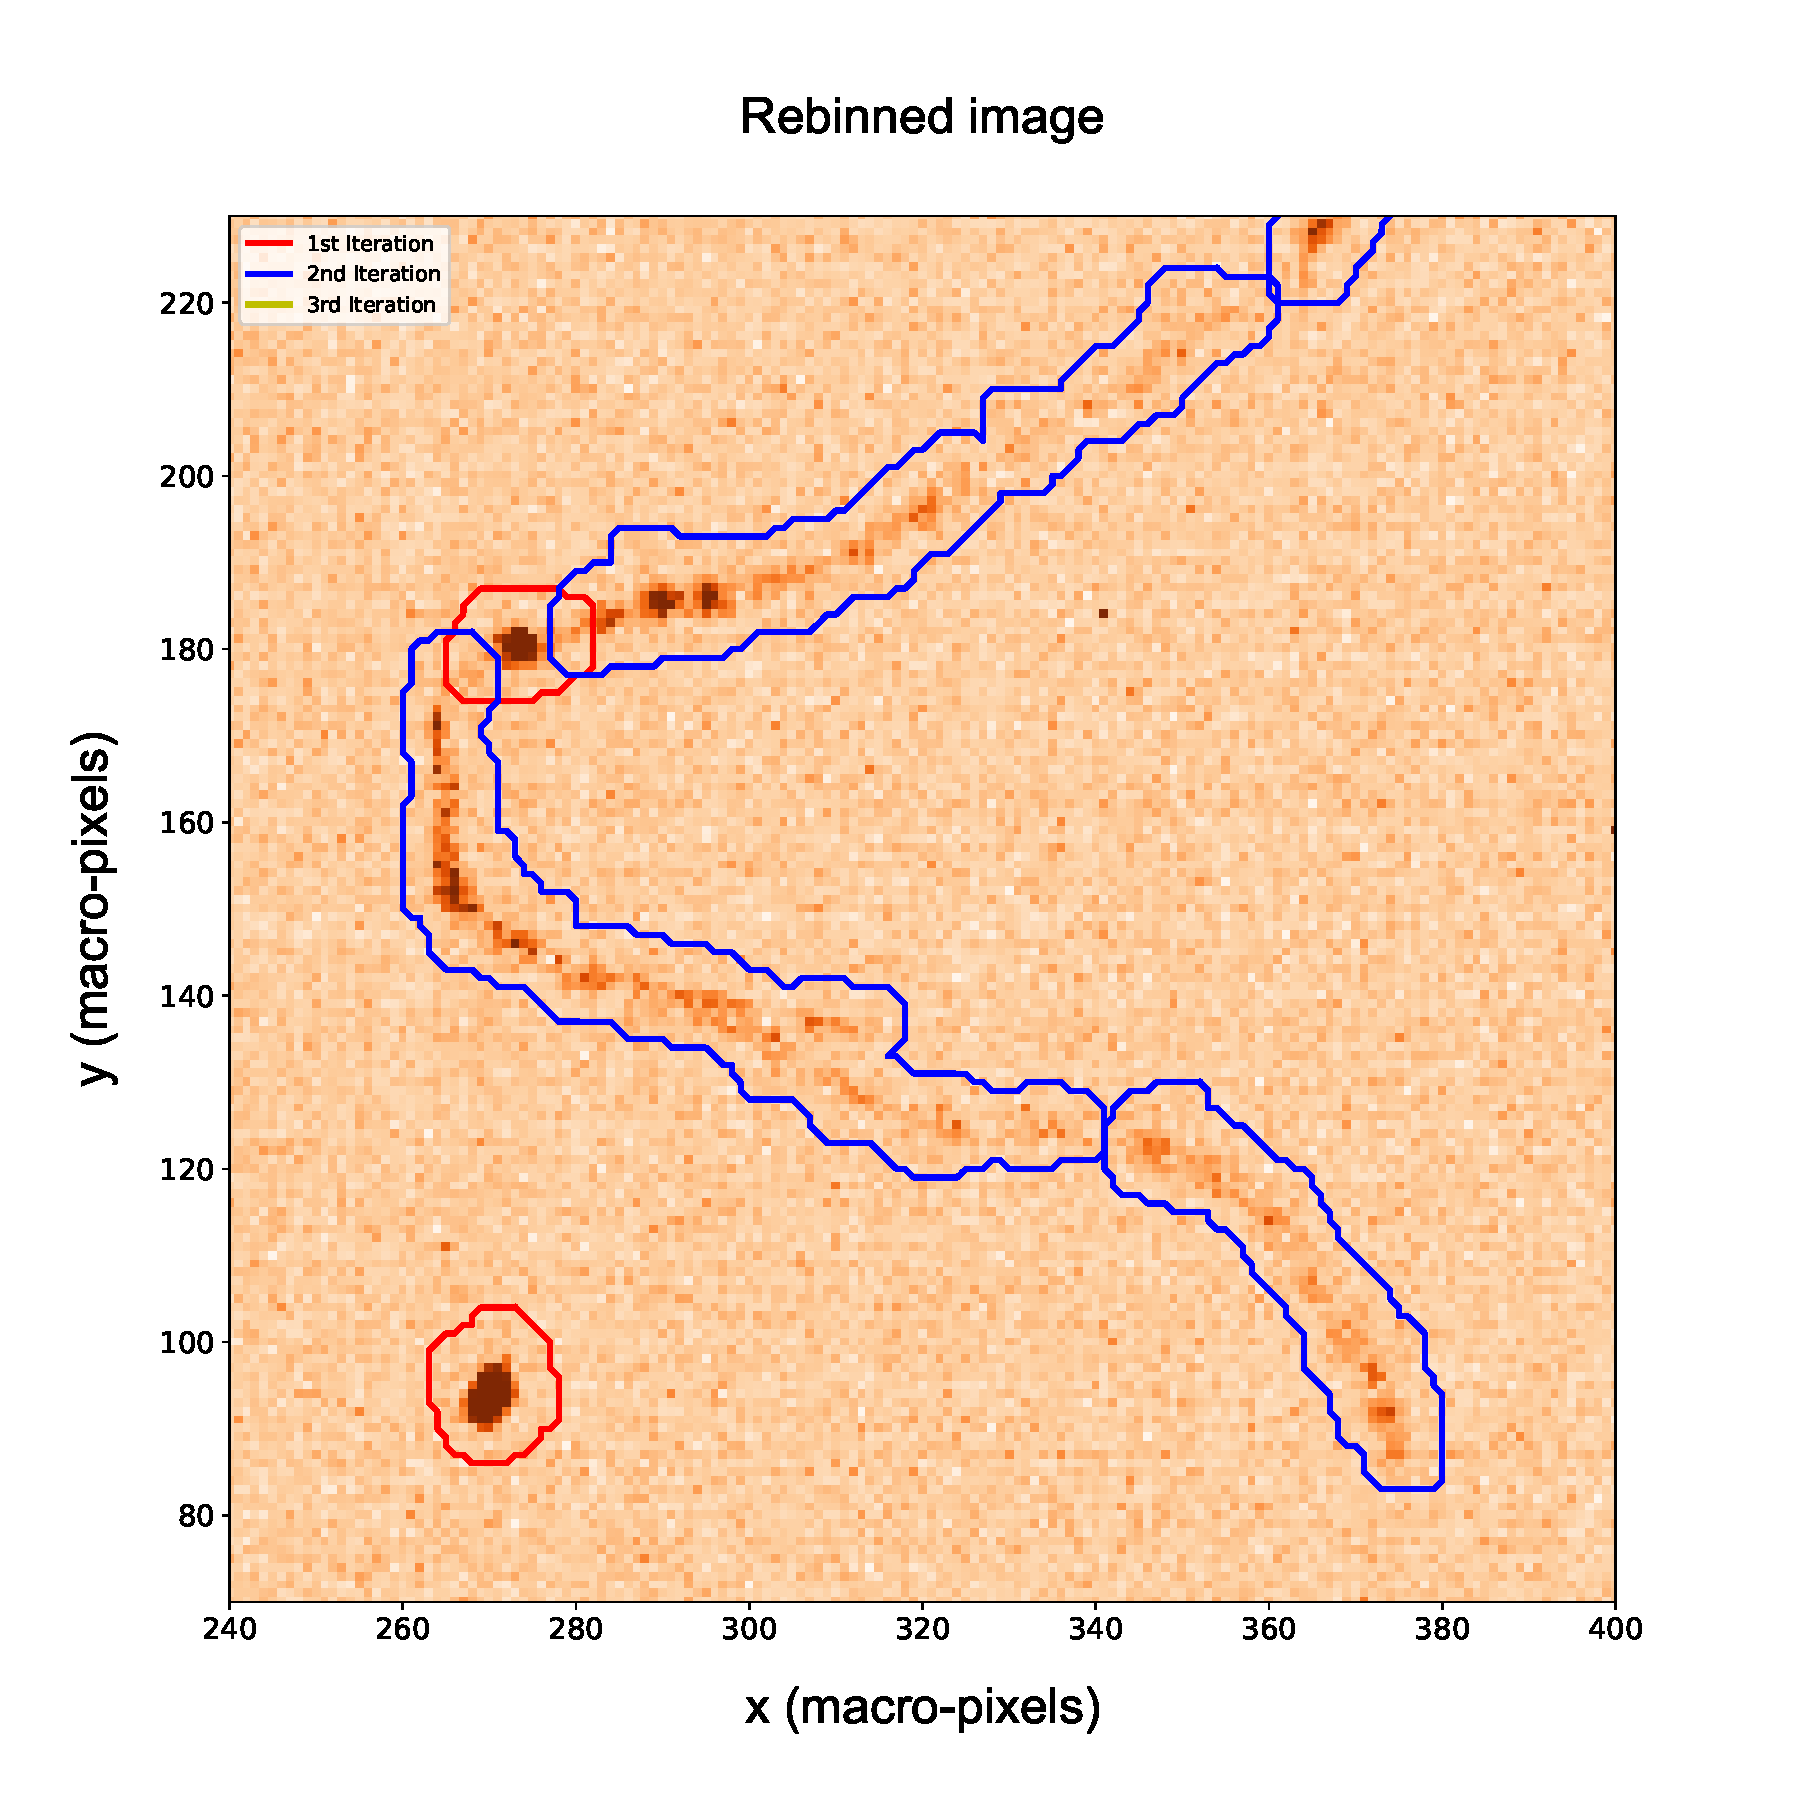
\includegraphics[width=0.49\linewidth]{figures/pic_run02317_ev8_all_3D_paper}

      \caption{Basic clusters reconstructed with the \idbscan
    algorithm in the low resolution (512$\times$512) image for two
    example events with very different patterns. Continuous lines
    represent the approximate contours of the reconstructed basic
    clusters of the first (red line) or second (blue line) \idbscan
    iteration. Left: clusters on spots from \fe source, two of which
    are merged together. Right: Track from natural radioactivity and a
    nuclear recoil candidate in an event with \ambe source. The long
    track is split in several basic clusters of different \idbscan
    iteration. \label{fig:basic_clusters}}

   \end{center}
\end{figure}



\subsection{Superclusters reconstruction}
\label{sec:supercl}
The aim of the superclustering procedure is to collect the majority of
the pixels belonging to a track which is long and can be split in
multiple parts in the clustering step described before.  Indeed, the
main limitation of \idbscan to follow a long track is mainly
originated by the non uniform energy release along the path length.
As can be clearly seen in Fig.~\ref{fig:basic_clusters} (right), or
even in the example of a raw image of an event with two long cosmic
rays in Fig.~\ref{fig:typicalimage1} (right), clusters with larger
energy release are followed by regions along the path with a lower or
even a zero release.  These local minima are sometimes as large, in
the 2D space, as the typical size of the $\epsilon$ parameter of
\dbscan~\cite{dbscan}. Despite the low electronic noise of the
\texttt{ORCA-Flash 4.0} camera sensor, the energy releases in these local
minima are similar in magnitude to the average single-pixel noise.

The \idbscan is limited in connecting the full length of an extended
path, because of two reasons. First, inflating $\epsilon$ parameter as
much as needed to cover the areas of local minima conflicts with the
need to reject noise around the cluster.  The basic cluster parameters
were optimized for the \lemon running conditions to collect most of
the signals with an energy as low as few keVs and to reject the
typical noise of $\approx 1$ photon per pixel. This avoids collecting
extra noise in the cluster, biasing the energy scale and worsening its
resolution, and keeps the rate of fake clusters at a negligible
level~\cite{iDBSCAN}.  Second, the iterative nature of the algorithm,
with different parameters for each iteration, each tuned for very
different intensity, makes it convenient and efficient for a
deposition of a fixed energy density (like the spots originating from
the \fe source), but not for the cases as in
Fig.~\ref{fig:basic_clusters} (right), where the same track is split
in several parts, some of them belonging to different iterations.
This requires a method that can continuously follow the pattern of the
track, profiting of the full resolution image, where the {\it
gradients} of the energy deposition along the track trajectory are
smaller than the ones in the transverse direction, but still give
information on the energy release pattern. Several existing algorithms
were tested to profit of this, but executing any of them on the full
$2048{\times}2048$ image is not manageable CPU-wise, due to the huge
pixel combinatorics.

Therefore, the procedure adopted for the final supercluster
reconstruction in the
\lemon detector starts from defining the \textit{interesting regions}
in the image that may contain pixels from an energy deposit. These are
identified by the basic cluster algorithm \idbscan previously
described, which is applied on the $512{\times}512$ reduced-resolution
image. In order to gather the peripheral pixels, especially along the
track trajectory where breaks into small basic clusters may have
happened, a window of $5{\times}5$ pixels is considered, around each
pixel belonging to a macro-pixel clustered in a basic cluster. A full
resolution image formed only by the interesting pixels passing the
simple initial filtering described in Sec.~\ref{sec:zerosuppression}
is created.  The gradients of the intensity $N_{ph}$ in such image are
computed pixel-by-pixel to look for the edge region where the image
turns from signal to noise-only:
%
\begin{equation}
\label{eq:gradient}
\vert\vert\nabla(N_{ph})\vert\vert =
\sqrt{\left(\frac{\partial N_{ph}}{\partial x}\right)^2
  +\left(\frac{\partial N_{ph}}{\partial y}\right)^2},
\end{equation}
%
while the gradient direction is given by:
\begin{equation}
  \label{eq:graddir}
  \theta = \tan^{-1}\left(\frac{\partial N_{ph}}{\partial y}/\frac{\partial N_{ph}}{\partial x}\right).
\end{equation}
%
In order to reduce the effect of the noise, which induces fluctuations
in the first derivatives of Eq.~\ref{eq:gradient}, a Gaussian filter
is applied, which smoothen the response by convolving the pixel
intensity with a Gaussian function, having as $\sigma$ the SD of the
intensities of all the pixels considered, and rejecting the ones
falling outside a 5$\sigma$ window.

The superclustering algorithm, applied on the filtered image, is an
application of the \textit{morphological geodesic active
contours}\cite{gac,mgac}, called \gac in the following.  This method
uses an active contour finding, widely used in computer vision, where
the boundary curve $\mathcal{C}$ of an object is detected by
minimizing the \textit{energy} $E$  associated to $\mathcal{C}$:
\begin{equation}
  \label{eq:gacenergy}
  E(\mathcal{C}) = \int_{0}^{1} g(N_{ph})(\mathcal{C}(p)) \cdot \vert\mathcal{C}_p\vert dp,
\end{equation}
%where $N_{ph}$ is the number of photons in the pixel,
where $ds=\vert\mathcal{C}_p\vert dp$ is the arc-length
parameterization of the curve in the 2D space, and $g$ is the stopping
edge function, which allows to select the boundary of the cluster.  In
the \gac method used for the \lemon images, the $g$ function is purely
geometrical, and uses the geodesics of the image, \ie, the local
minimal distance path joining points with the same light intensity
gradient. The function $g(N_{ph})$ is given by:
\begin{equation}
g(N_{ph}) = \frac{1}{\sqrt{1+\alpha\vert\nabla G_\sigma * N_{ph}\vert}},
\end{equation}
which is minimal in the edges of the image.  The $G_\sigma * N_{ph}$ is the
aforementioned $5\sigma$ Gaussian filter, and the parameter $\alpha$,
which regulates the strength of the filter, was tuned on
typical \lemon images to be $\alpha=100$.

This method was chosen because it allows to follow patterns that
may vary from convex to concave shape, eventually with kinks, \eg in
cases of $\delta$-ray emissions. To improve the shrinking of the
cluster boundary in the cases of tracks turning from concave to convex
along their trail, the \textit{balloon} force~\cite{mgac}, which is a
term added to Eq.~\ref{eq:gacenergy} to smooth the cluster contour, is
set to -1, in order to push the contour towards a border in the areas
where the gradient is too small. A number of 300 iterations is used to
evolve the supercluster contour.

The example track shown in Fig.~\ref{fig:basic_clusters} (right) after
the basic clustering step, is shown again in full resolution, zoomed
around the cluster, in Fig.~\ref{fig:super_clusters1} (left). The
output of the superclustering with the \gac algorithm is shown on the
right panel of the same figure. The splitting of the cluster,
happening at the basic clusters step, is recovered: the portions with
high and low density along the path of the energy release are joined
together. Other three examples of superclustered images are shown in
Fig.~\ref{fig:super_clusters2}, in runs without any artificial
radioactive source. The top left panel shows an example of a cosmic
ray track fully reconstructed by the \gac superclustering, which also
includes a $\delta$-ray in the middle of the track length. The top
right panel shows an example of curly track from a candidate of
natural radioactivity interaction; bottom panel shows an example where
both a cosmic ray and a curly track are present. In this case, the
extremes of the long and straight track are still split, but this is
much rarer than after the basic clustering, and it happens when the
local minima along the trajectories are compatible with noise-only
for more than $\approx$1\unit{cm}.
%
\begin{figure}[ht]
  \begin{center}
     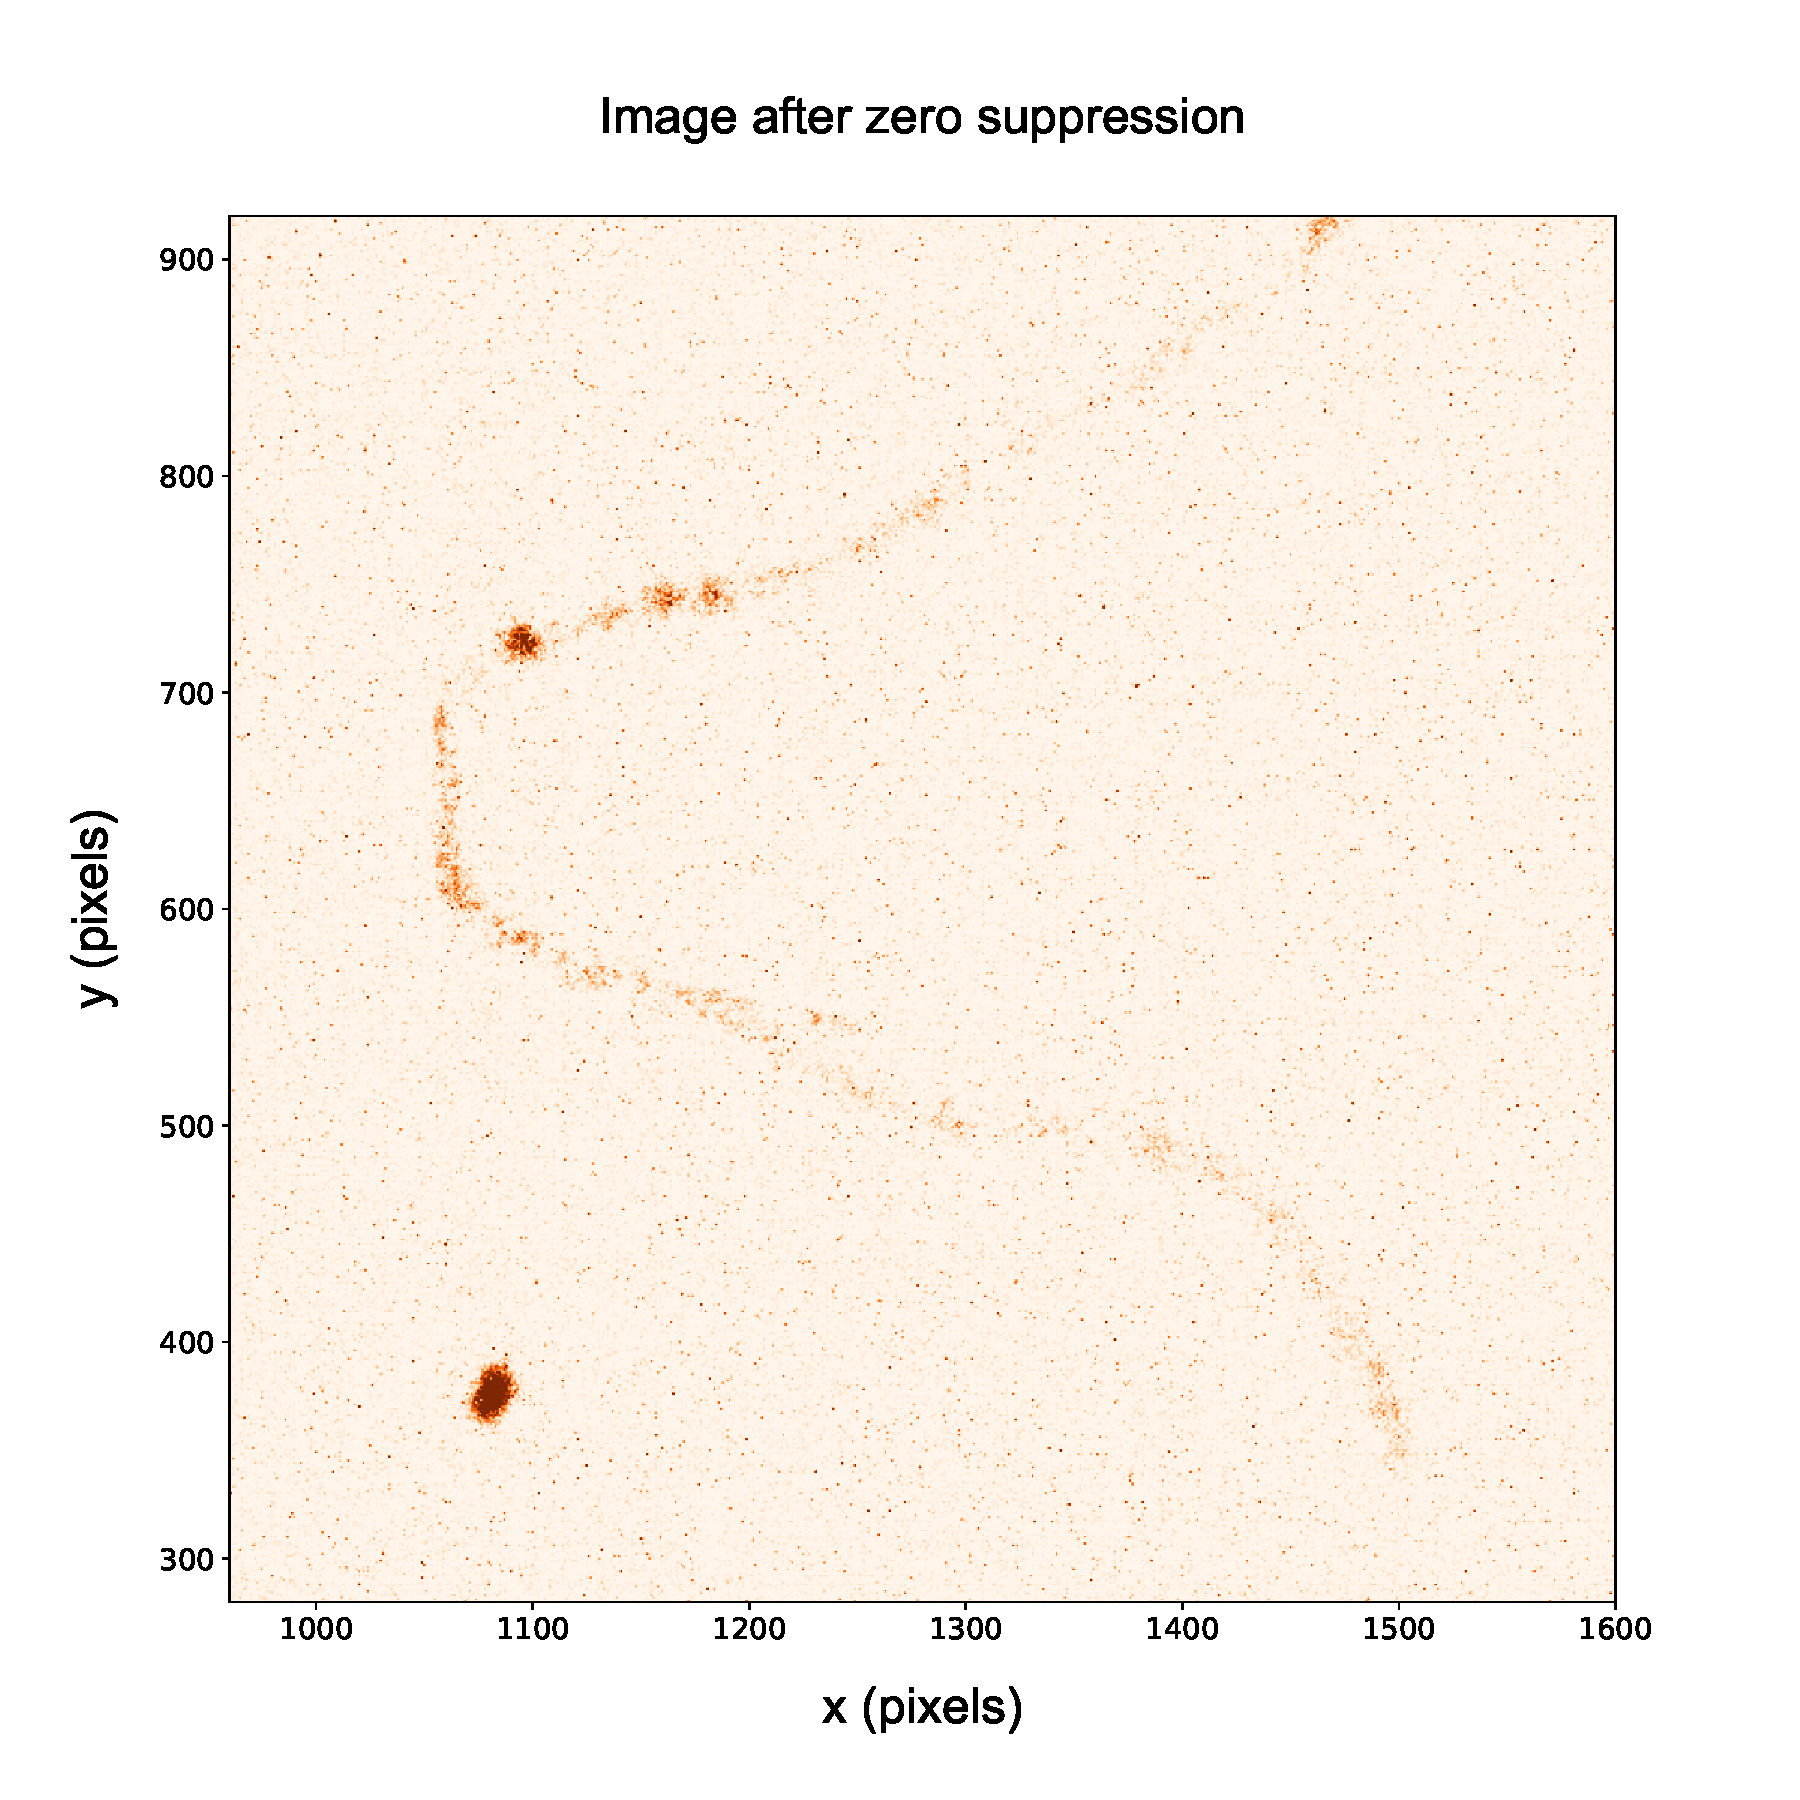
\includegraphics[width=0.49\linewidth]{figures/pic_run02317_ev8_oriIma_paper_zoom}
      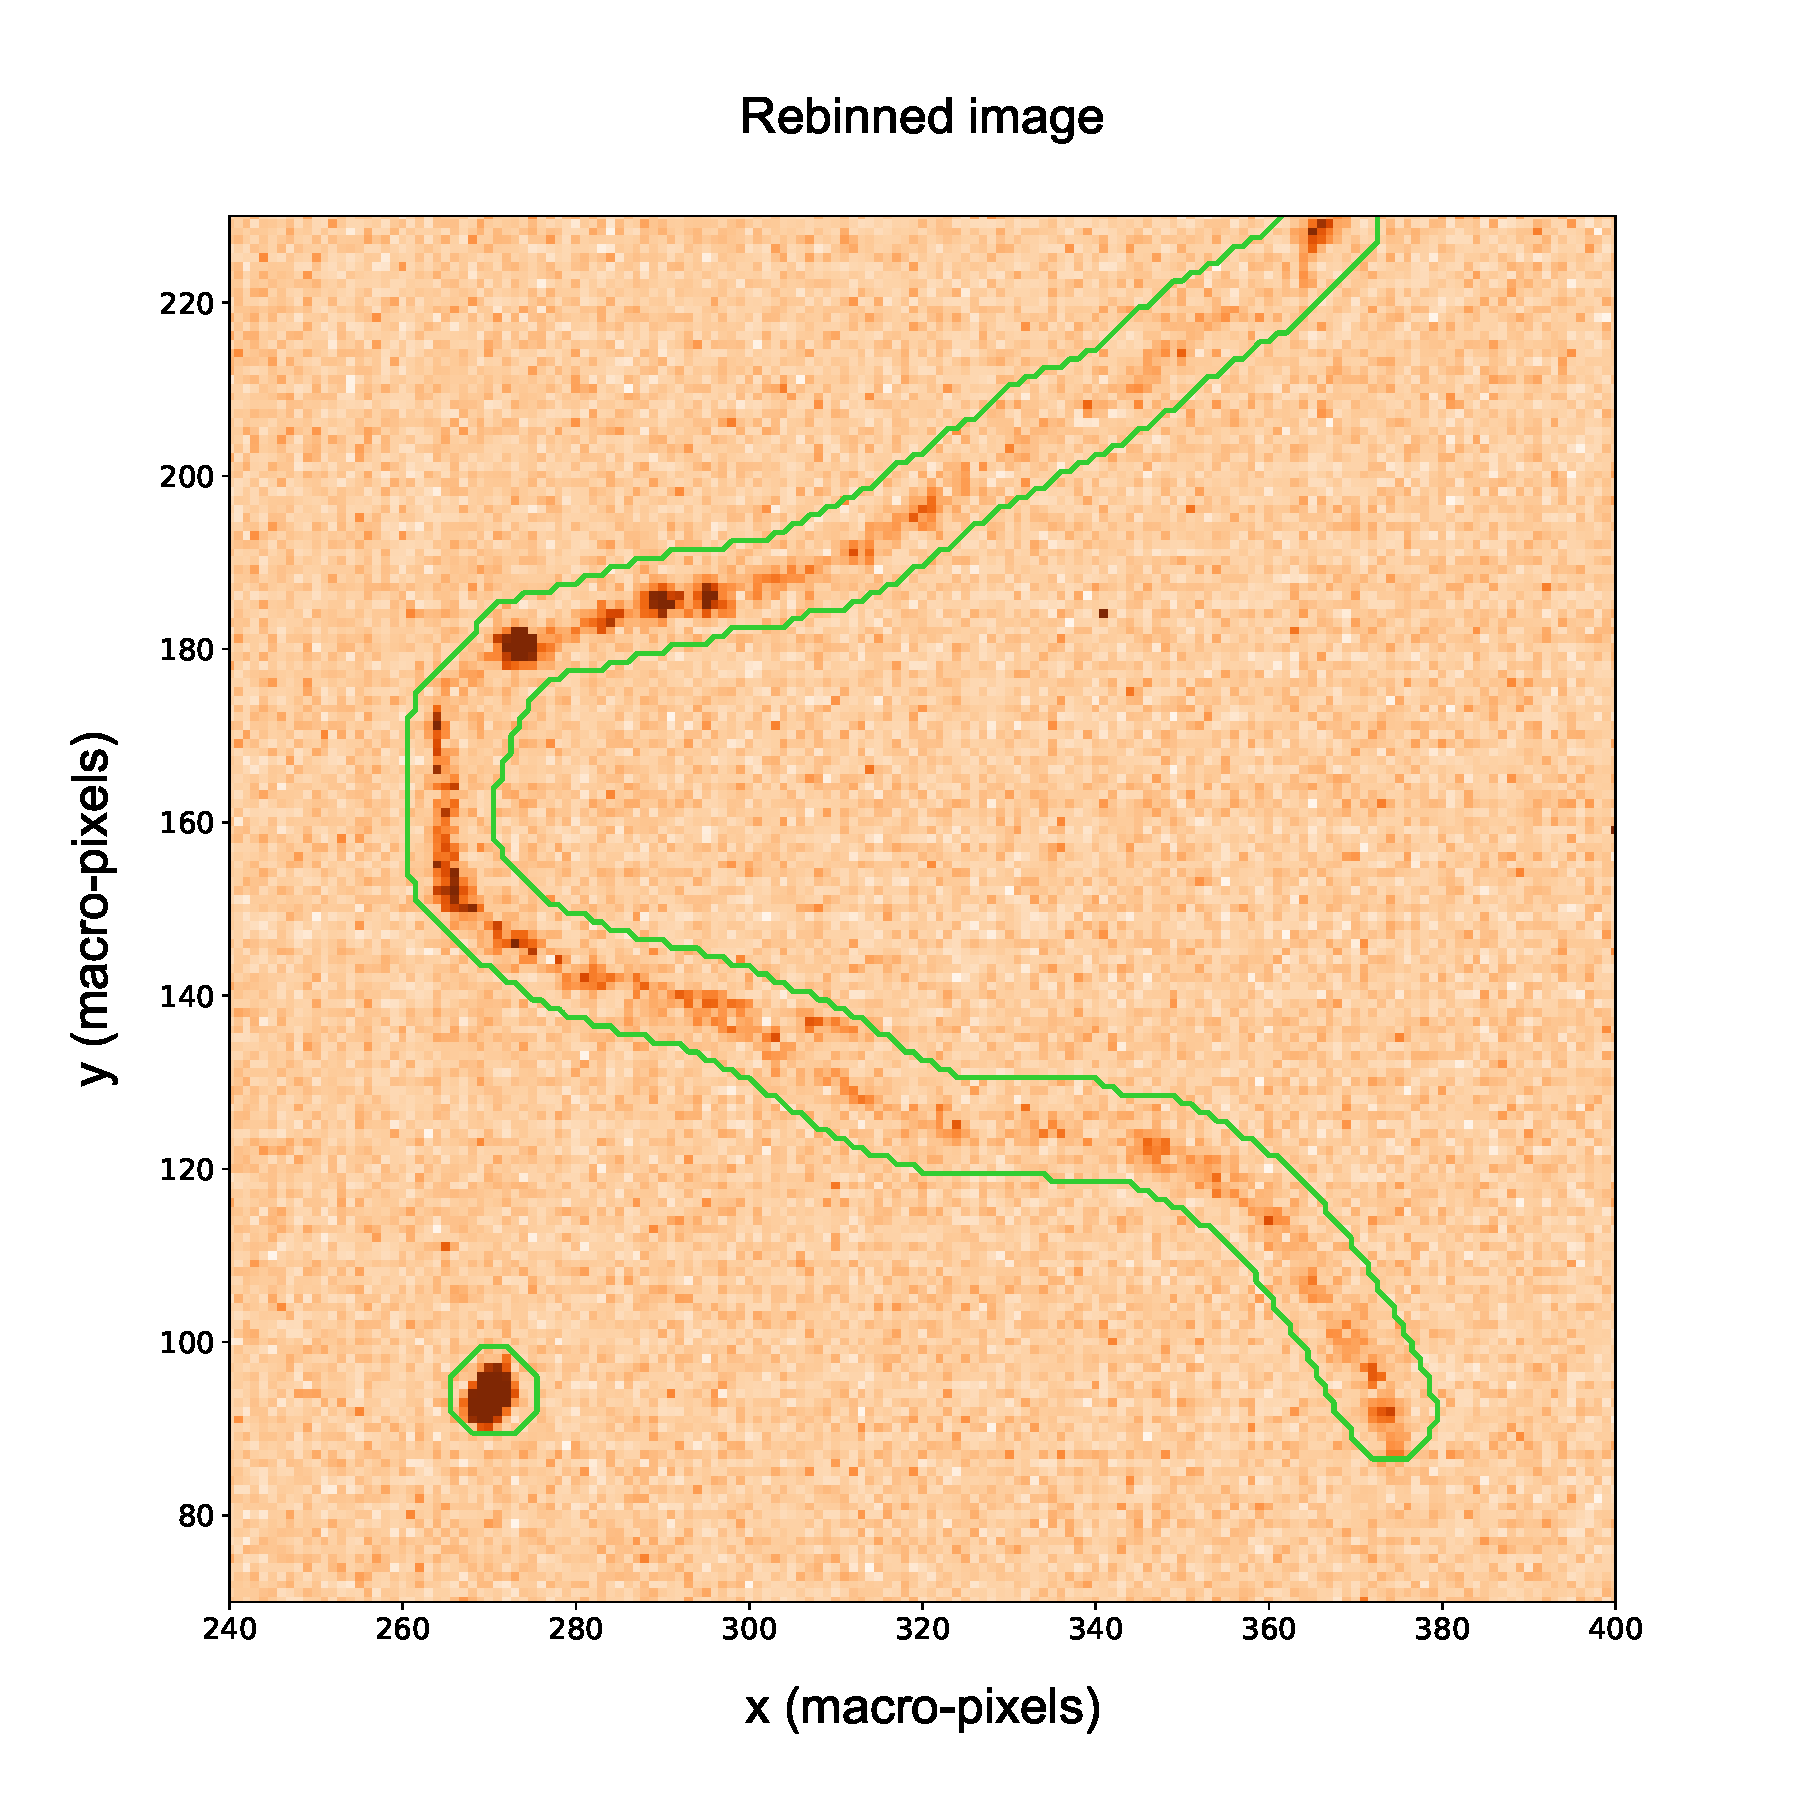
\includegraphics[width=0.49\linewidth]{figures/pic_run02317_ev8_sc_3D_paper}
      \caption{Left: zoom on the full-resolution image of a track
        candidate in a run with the \ambe radioactive source. Right:
        output of the superclustering on the rebinned image. The
        continuous line represents the approximate contour of the
        reconstructed supercluster. \label{fig:super_clusters1}}
  \end{center}
\end{figure}
%
\begin{figure}[ht]
  \begin{center}
     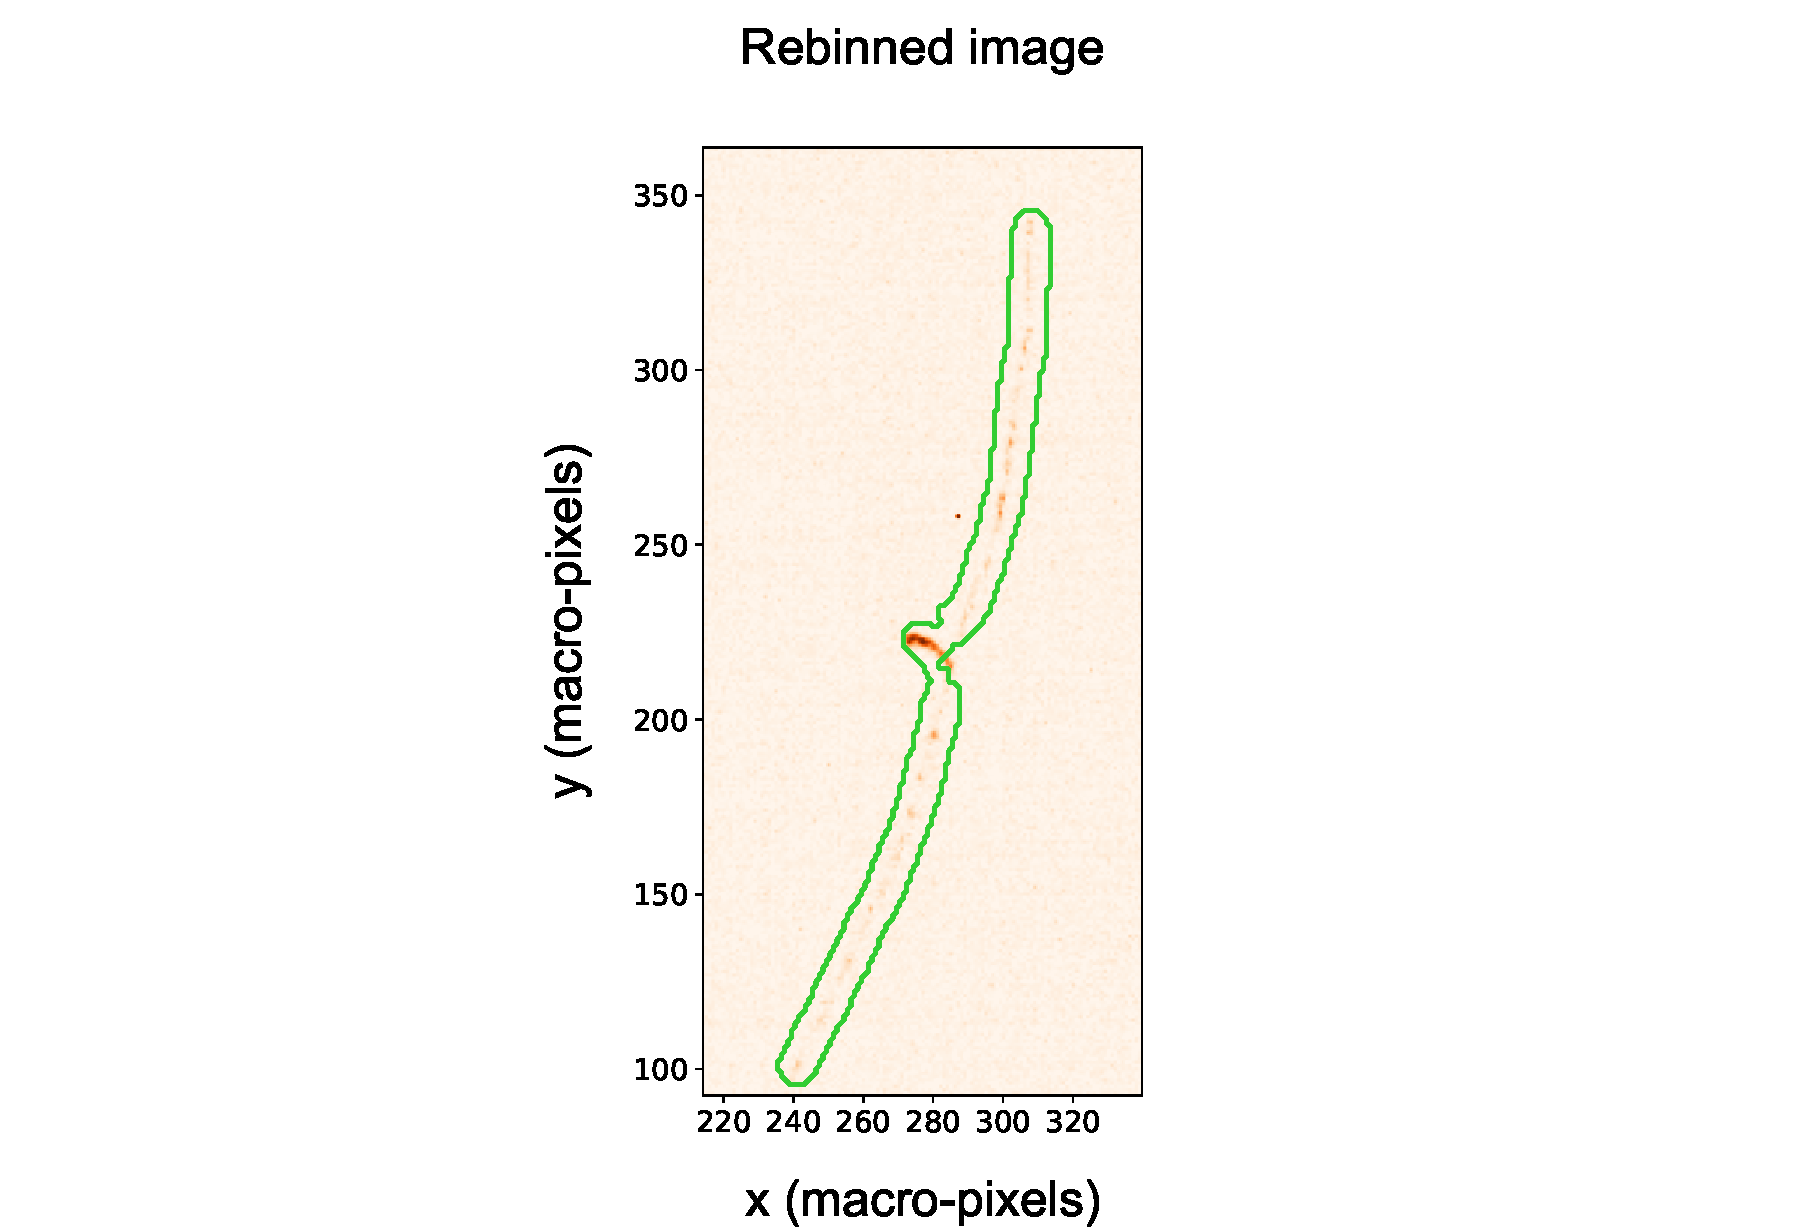
\includegraphics[width=0.49\linewidth]{figures/pic_run02156_ev49_sc_3D_paper}
     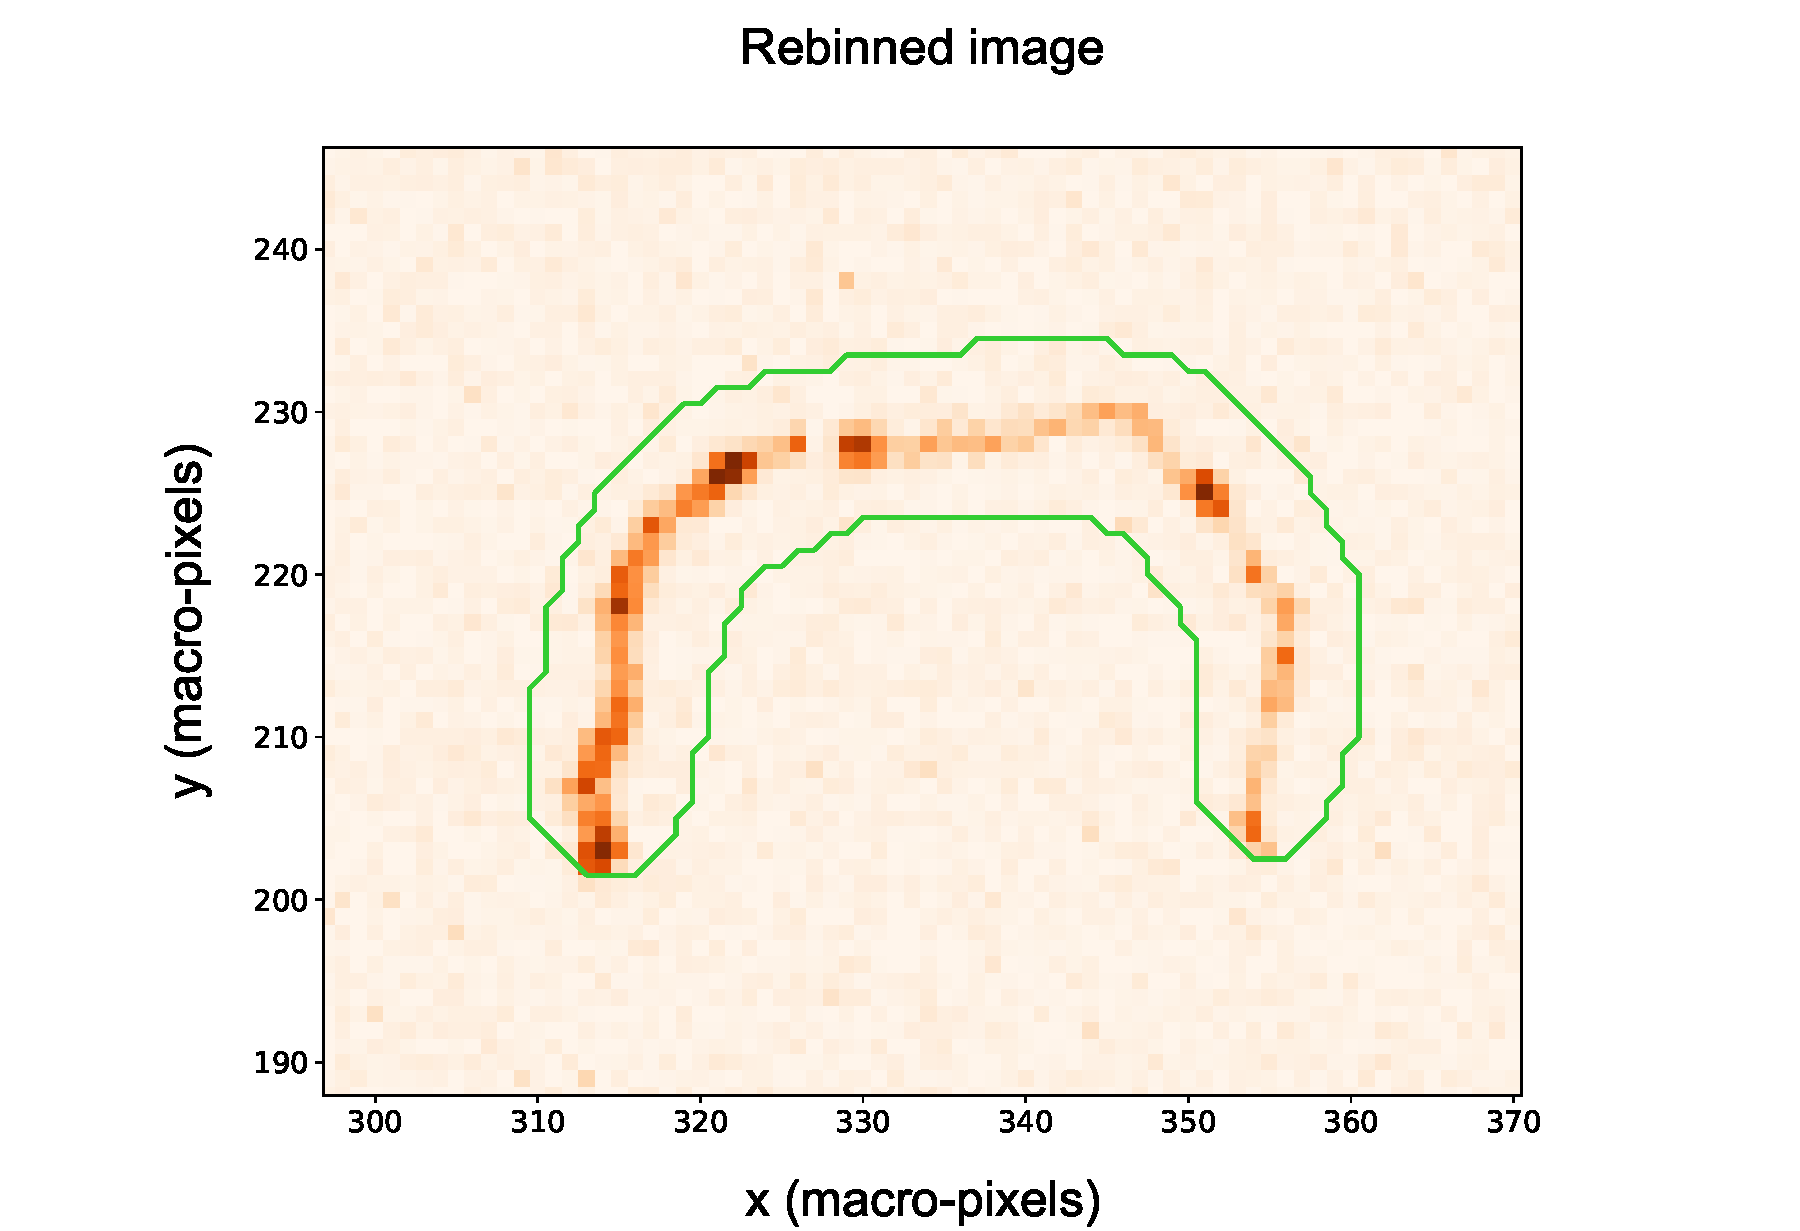
\includegraphics[width=0.49\linewidth]{figures/pic_run02156_ev641_sc_3D_paper} \\
     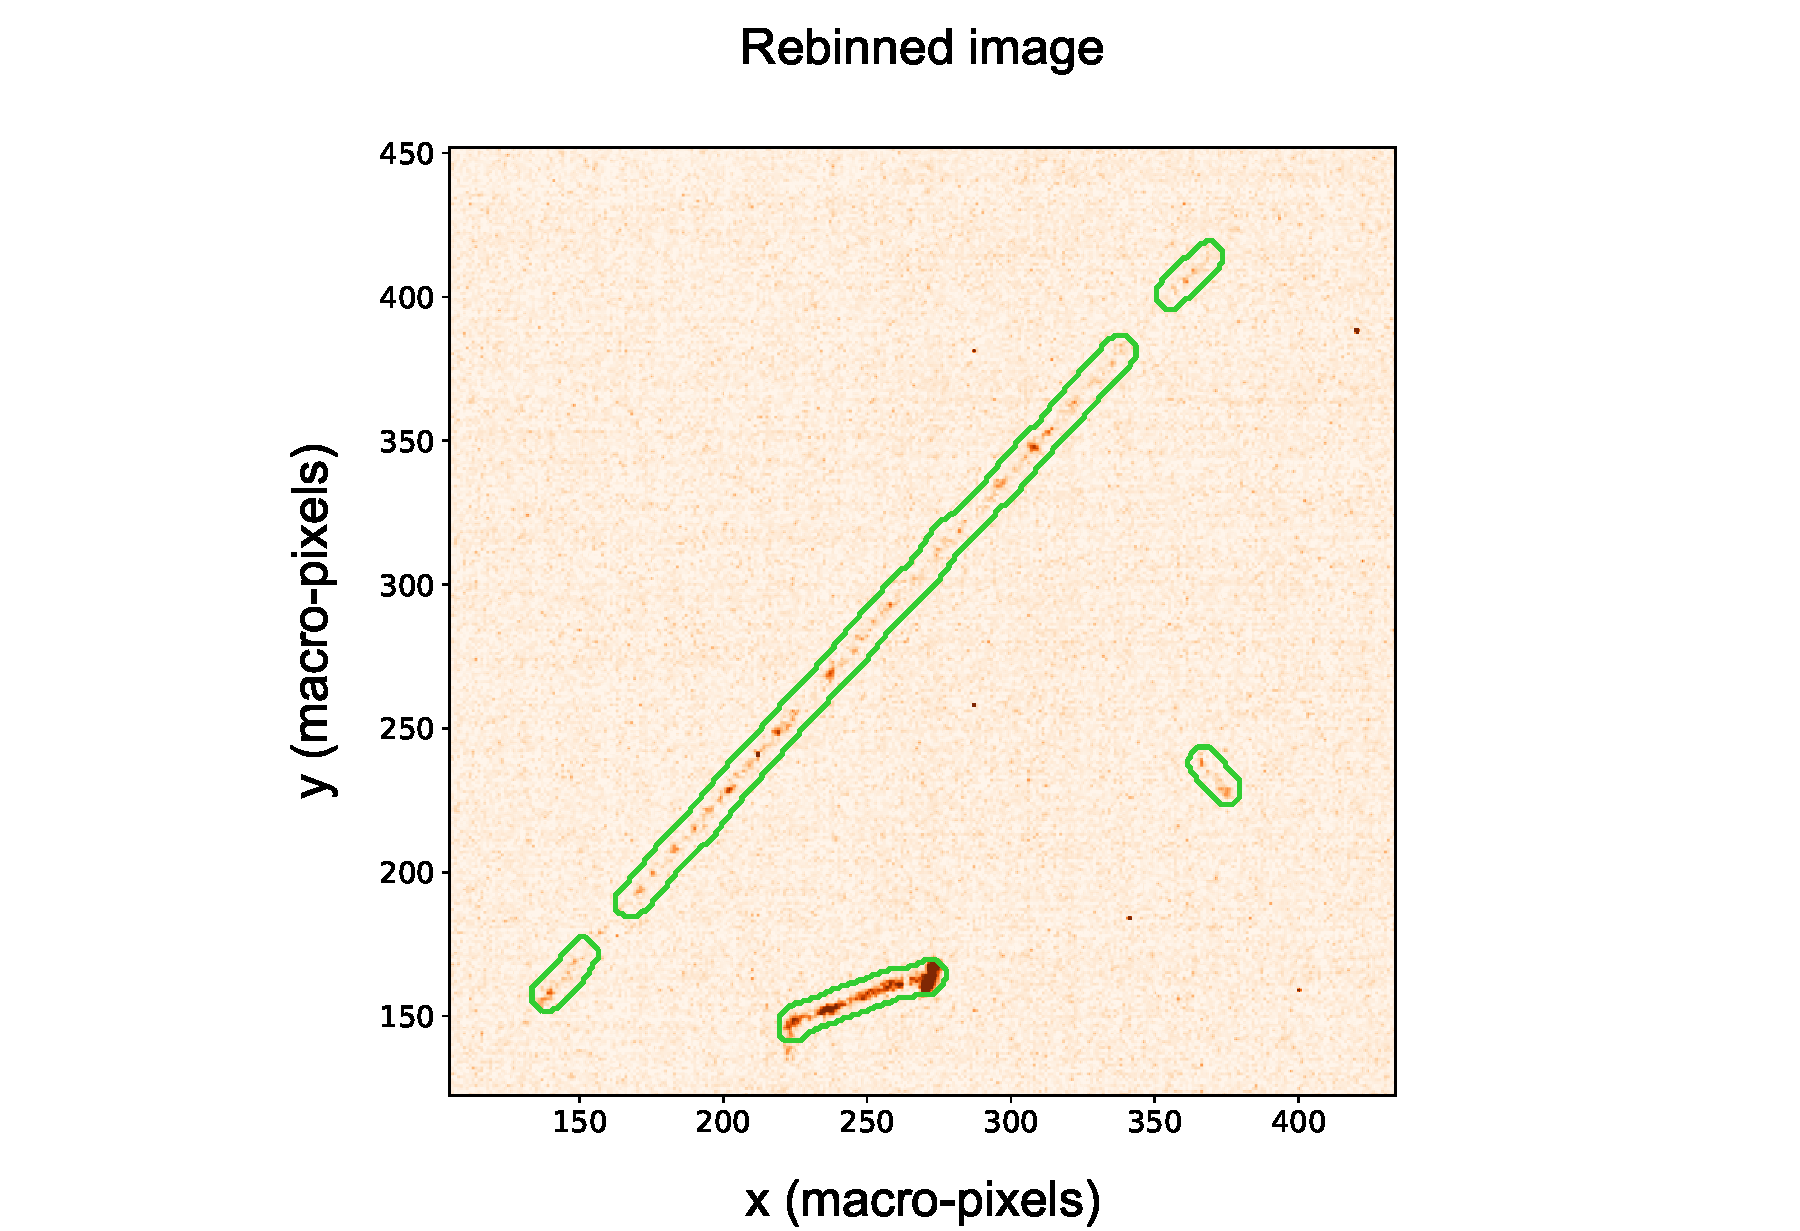
\includegraphics[width=0.6\linewidth]{figures/pic_run02156_ev631_sc_3D_paper}

     \caption{Superclusters reconstructed in a run without artificial
       radioactive sources. The continuous lines represent the
       approximate contours of the reconstructed superclusters. Top
       left: cosmic ray track fully reconstructed by the \gac
       superclustering. A $\delta$-ray is included in the
       supercluster. Top right: curly track from a candidate of
       natural radioactivity interaction. Bottom: a cosmic ray with
       the extremes not joined to the main track, plus a curly track
       from natural radioactivity. \label{fig:super_clusters2}}
       
  \end{center}
\end{figure}


\clearpage

\subsection{Superclusters calibration}
\label{sec:calibration}
The containment of the energy in the supercluster was verified
with simulations  performed with
\SRIM~\cite{bib:srim} of nuclear and electron recoils  within the gas mixture of the \lemon detector.
For both types of recoils, for the energy range of interest for DM
 search, \eg $E<10\keV$, when considering deposits without electronics
 noise and no diffusion in the gas, the peak of the
 $\abs{E-E_{true}}/E_{true}$ is within 5\%. Adding a Gaussian noise
 distribution with a mean equal to the one observed in the pedestal
 runs, and a diffusion following the parameterization in
 Eq.~\ref{eq:diff}, the fraction of the true energy contained in the
 supercluster decreases to about 80\%, as shown in
 Fig.~\ref{fig:eoveretrue}. The distributions were obtained for
 nuclear recoils with $E=6\keV$ generated at the exact center of
 the \lemon detector. The mean and the Gaussian width of the peak are
 estimated by fitting the distributions with a Crystal Ball
 shape~\cite{Oreglia:1980cs,Gaiser:1982yw}, which includes a tail to
 consider a non-Gaussian asymmetric tail due to partial containment in
 the supercluster.

The decrease in the energy containment in the supercluster is due to
the smearing of the 2D track pattern around the periphery of the
cluster.  This decreases the gradients in Eq.~\ref{eq:gradient} around
the edges, and so the supercluster can shrink more around the crest,
loosing part of the tails that can be confused more easily with the
noise.  A more realistic noise description, and an improved diffusion
model, based on the one measured in data is necessary to tune the
supercluster parameters in simulation to recover part of the
containment. Despite this, the resolution in presence of noise and
diffusion is estimated in this simulated nuclear recoils with
$E=6\keV$ to be around 4\%. This energy resolution is expected to be
very optimistic because the absence, in the simulation, of the
dominant fluctuations of the GEM gain.
%
\begin{figure}[ht]
  \begin{center} 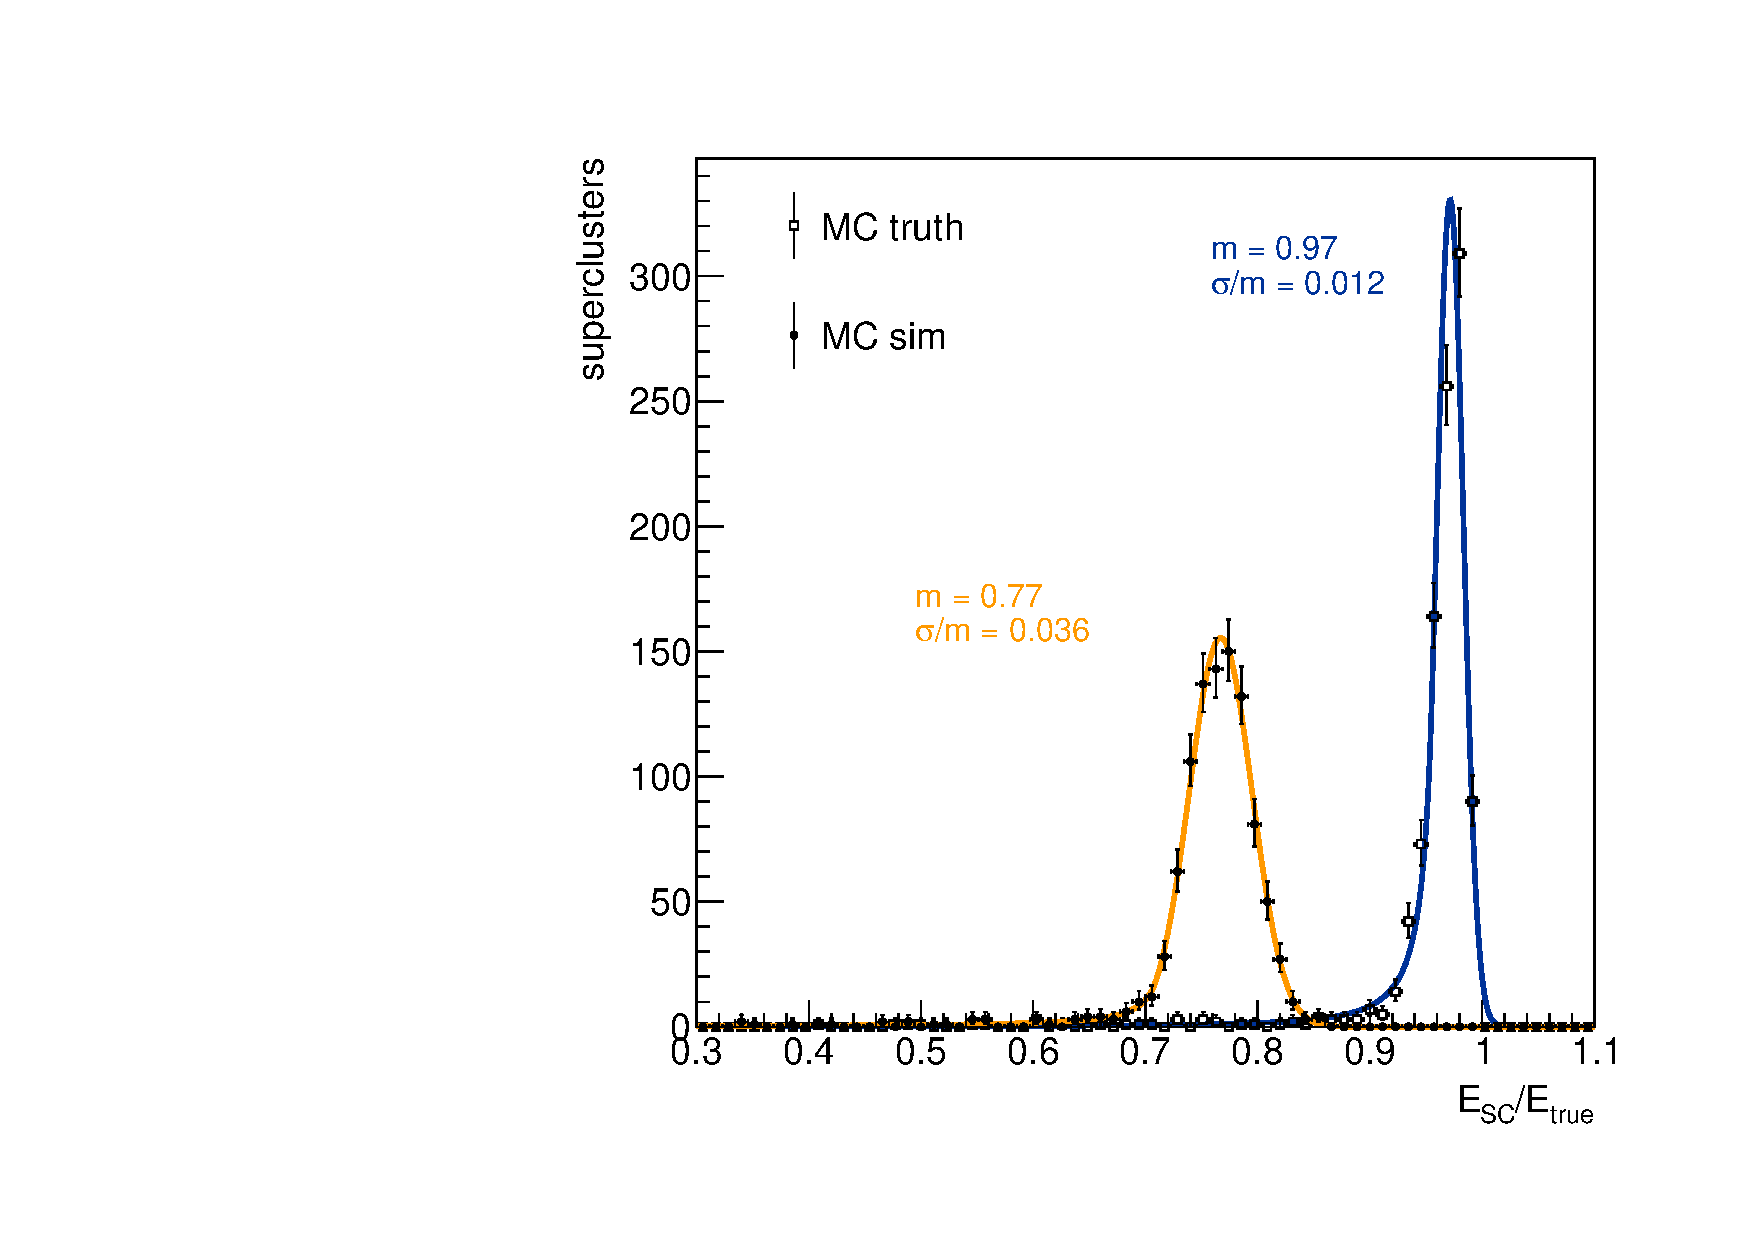
\includegraphics[width=0.49\linewidth]{figures/eoveretrue}
   \caption{Distribution of the ratio of reconstructed supercluster
    energy, $E$, and the true energy of nuclear recoils
    $E_{true}=6\keV$, generated in the center of \lemon and simulated
    with \GEANTfour Monte Carlo (MC). The hollow points show the MC
    events generated without electronics noise and diffusion in the
    gas, while the filled circles represent MC events with both
    effects included. The curves represent parametric fits with a
    Crystal Ball function.\label{fig:eoveretrue}}
  \end{center}
\end{figure}
%

The absolute energy scale was then calibrated with the energy distribution
measured in data with the \fe source, which provides monochromatic
photons of 5.9\keV, with the procedure described in
Ref.~\cite{bib:fe55}. The supercluster integral is defined as:
\begin{equation}
\label{eq:integral}
I_{SC} = \sum_i^{cluster} N_i,
\end{equation}
where $N_i$ is the number of counts (photons) in the $i^{th}$ pixel,
and the sum runs over all the pixels of the supercluster.  While to
perform the basic- and super-clustering only pixels passing the zero
suppression are considered, for the energy estimate in
Eq.~\ref{eq:integral} all the pixels within the cluster contours are
counted, eventually having negative $N_i$, after the pedestal
subtraction. This is done to avoid a bias on the energy estimate.
The distribution of \isclu, for a run taken in presence of \fe source,
is shown in Fig.~\ref{fig:feuncalibpeak}.
%
\begin{figure}[ht]
  \begin{center}
    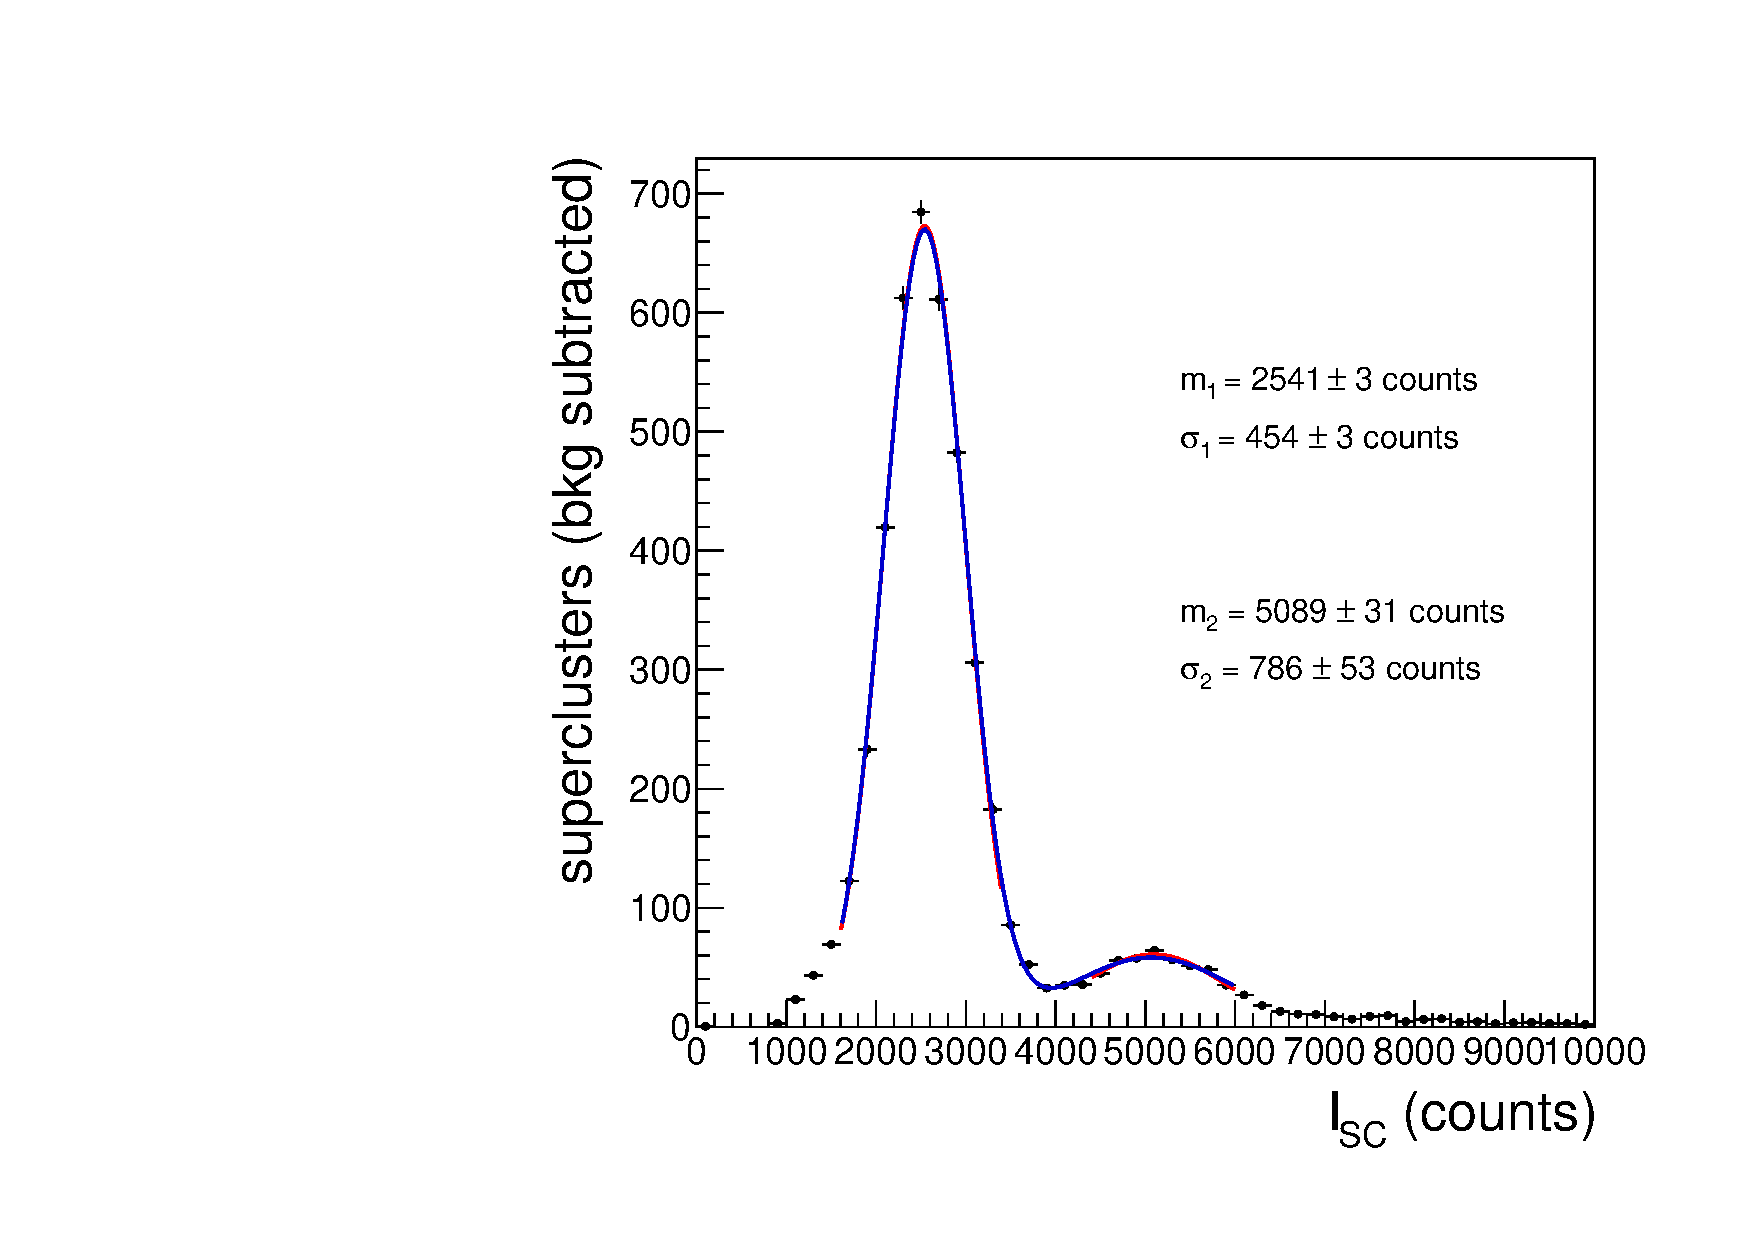
\includegraphics[width=0.49\linewidth]{figures/fe_ucalibintegral_fit}
    \caption{Distribution of the supercluster integral, before the
      absolute energy scale calibration is applied, in events with the
      \fe source. Clearly visible is the large peak of a single spot,
      and, at around twice the energy, a broader peak for the case of
      two neighboring spots merged in a single supercluster.
      \label{fig:feuncalibpeak}}
  \end{center}
\end{figure}
%
 The position of the maximum in the single-spot distribution in runs
with \fe source allowed to calibrate the absolute energy scale of
the \lemon detector.  The energy resolution for the reconstructed \gac
superclusters is about 18\%, similar to the one that can be obtained
with only the basic clustering step with \idbscan~\cite{iDBSCAN}, and
improving the one with the simple \nnc algorithm previously
used~\cite{bib:fe55}. This value is still much larger than the one
obtained with the simulation of nuclear recoils at the same energy,
but an improved noise and gas diffusion model, and a simulation of the
gas gain fluctuations are needed to improve the data-MC agreement.


Using runs with this monochromatic, high rate source, positioned at
different distances from the GEM planes, a decrease of the light
response for lower distances from the GEM was observed. This effect is
opposite to the expected behavior of a decreasing light yield at
larger distances. Indeed, it is expected that during the drift along
the $z$-direction the ionization charge undergoes a diffusion in the
TPC gas and some electrons are removed by attachment to the gas
molecule.  Consequently some loss in the light collection may be
expected. The opposite behavior, instead, is clearly observed. While
this effect is currently under study in more detail, it was attributed
to a possible saturation effect of the GEMs, especially in the third
stage of multiplication, for which the charge density in one GEM hole
is maximal.  Under this hypothesis, an effective, empirical correction
was developed, which relies on the charge density of a cluster from
a \fe deposit. The light density, $\delta$, is defined as:
\begin{equation}
  \label{eq:density}
  \delta = \isclu / n_p,
\end{equation}
where $n_p$ is the number of pixels passing the zero-suppression
threshold (differently from the numerator, where all the pixels in the
supercluster are considered). This effective calibration provides the
absolute energy of a spot-like region similar to the \fe ones, as a
function of the supercluster density, $\delta$: $E=c(\delta)\cdot
I_{SC}$. In the hypothesis of saturation, the
\textit{local} density along the track is the parameter which
regulates the magnitude of the effect, thus the correction has to be
applied dynamically for slices of the supercluster having a size
similar to the \fe spots.  This is achieved with the procedure
described in the following.

First, the supercluster \textit{skeleton}, \ie, the 1 pixel wide
representation along the energy deposition path, is reconstructed.
This is performed with a morphological thinning of the superclusters
with the iterative algorithm from Ref.~\cite{thin1,thin2}.  Second, a
pruning of the obtained skeleton is done, to remove residual branches
along the main pattern, using a hit-or-miss transform.  The output of
the \textit{skeletonization} for the track of
Fig.~\ref{fig:super_clusters1} is shown in Fig.~\ref{fig:skeleton}.
%
\begin{figure}[ht]
  \begin{center}
     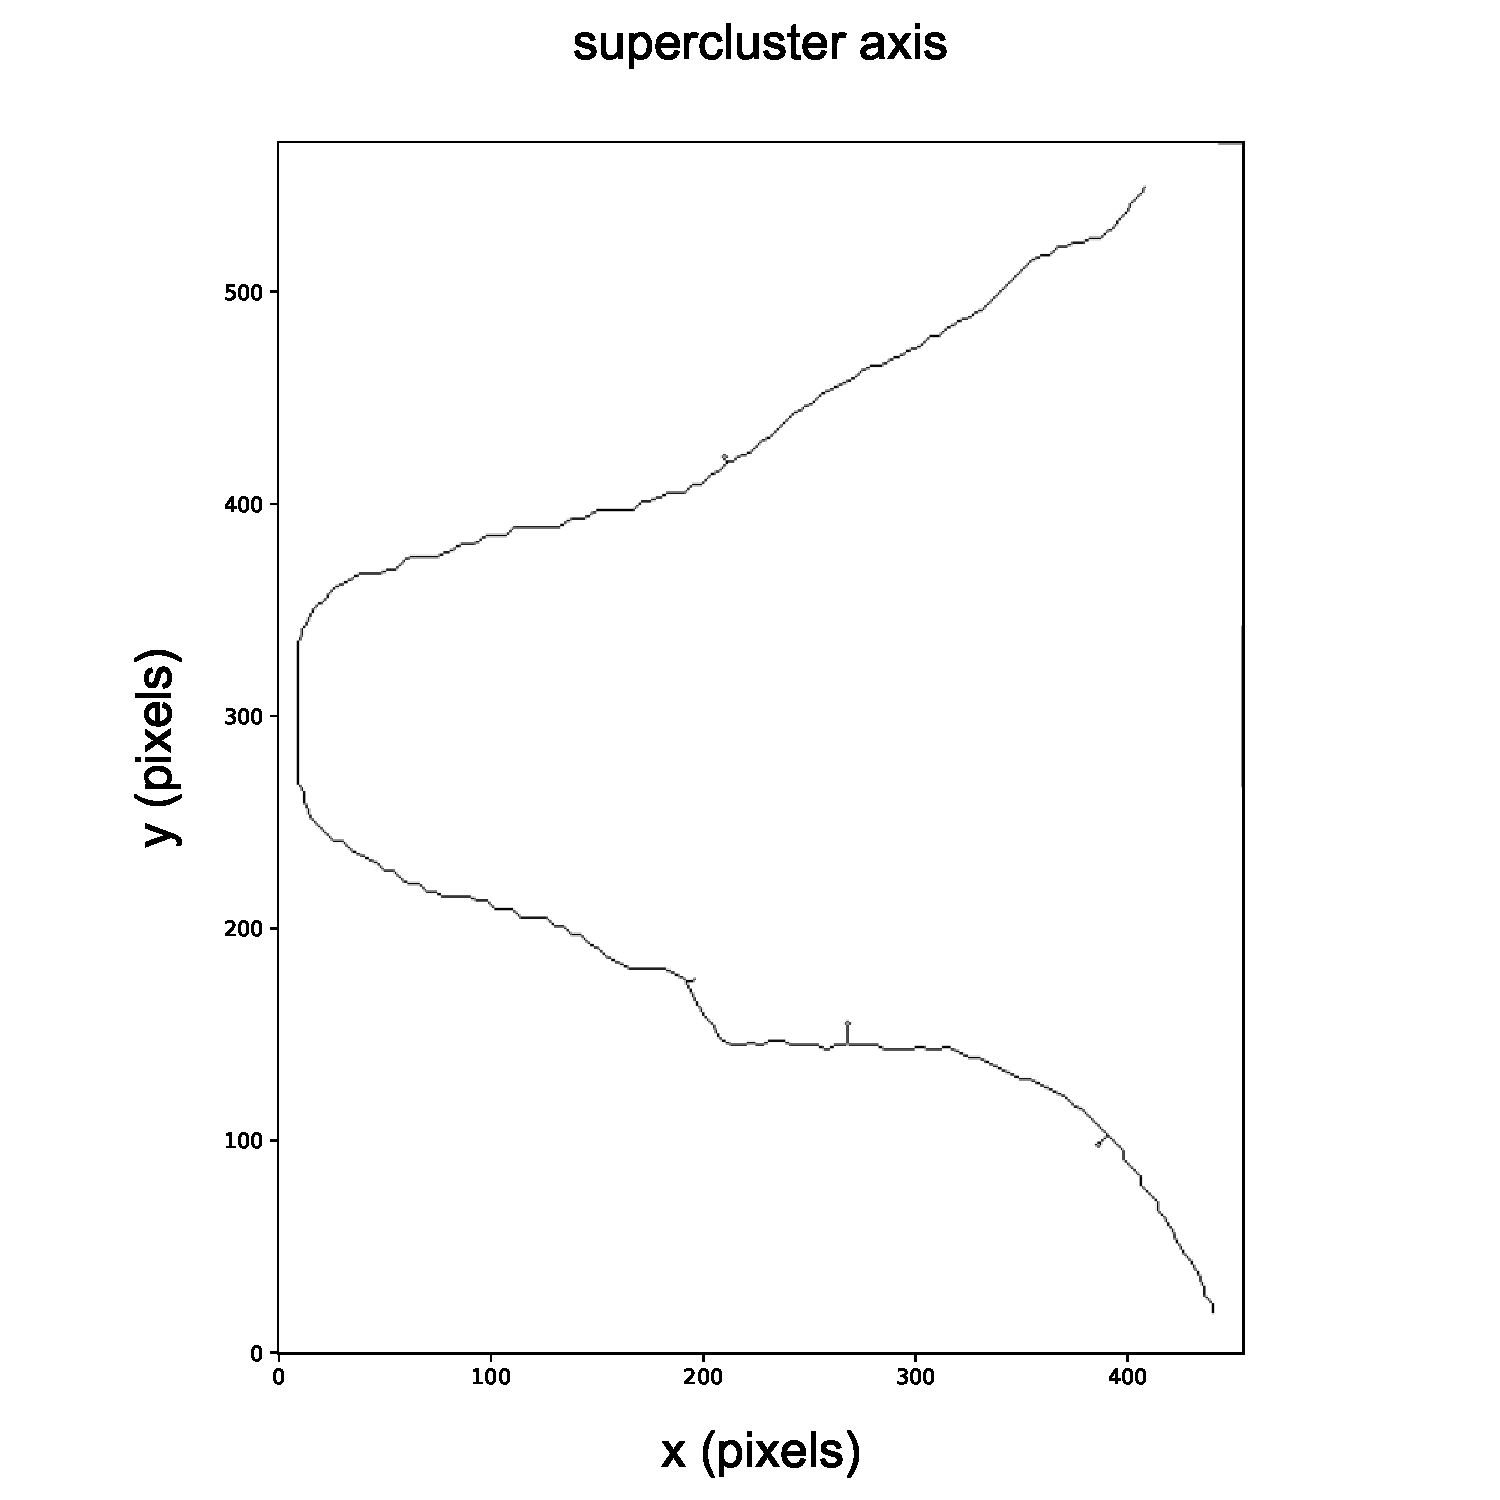
\includegraphics[width=0.49\linewidth]{figures/skeleton_paper}
     \caption{Output of the skeletonization and pruning of the
       branches for one example supercluster extended in
       space.  \label{fig:skeleton}}
  \end{center}
\end{figure}
%
For the calibration procedure, the skeleton was followed, starting
from one of the two end points, and circles having their center on a
pixel of the skeleton and their radius equal to the average spot size
of the \fe clusters were defined. The local density $\delta_s$ of the
slice $s$ is computed, and its integral $I_s$ is calibrated to an
absolute energy through the effective correction $E_s=c(\delta_s)\cdot
I_s$. The pixels of the supercluster used for the slice calibration
are removed (including the skeleton ones), and the procedure is
iterated, until having included all the pixels. The sum of the
energies of all the slices is the estimate of the calibrated energy of
the supercluster:
%
\begin{equation}
  \label{eq:ecal}
  E_{SC} = \sum_s^{slices} E_s
\end{equation}
%
As a closure test of this procedure, the calibrated energy of the
superclusters reconstructed in the runs with the \fe source is
obtained.  The value of the energy peak was obtained by fitting the
distribution with the same function used in
Fig.~\ref{fig:feuncalibpeak}, and equals to  $m_1 = 5.93 \pm 0.01$\keV,
compatible with the expected value. The calibration procedure is an
overkill for the case of the small \fe spots, but it is necessary for
very long cosmic ray tracks or even for medium-length superclusters
from nuclear and electron recoils.  The energy resolution worsen after
the calibration ($\sigma_1 = 1.48 \pm 0.01$, \ie, 25\% energy
resolution), as a sign that the empiric correction is still
suboptimal.
%
%% \begin{figure}[ht]
%%   \begin{center}
%%     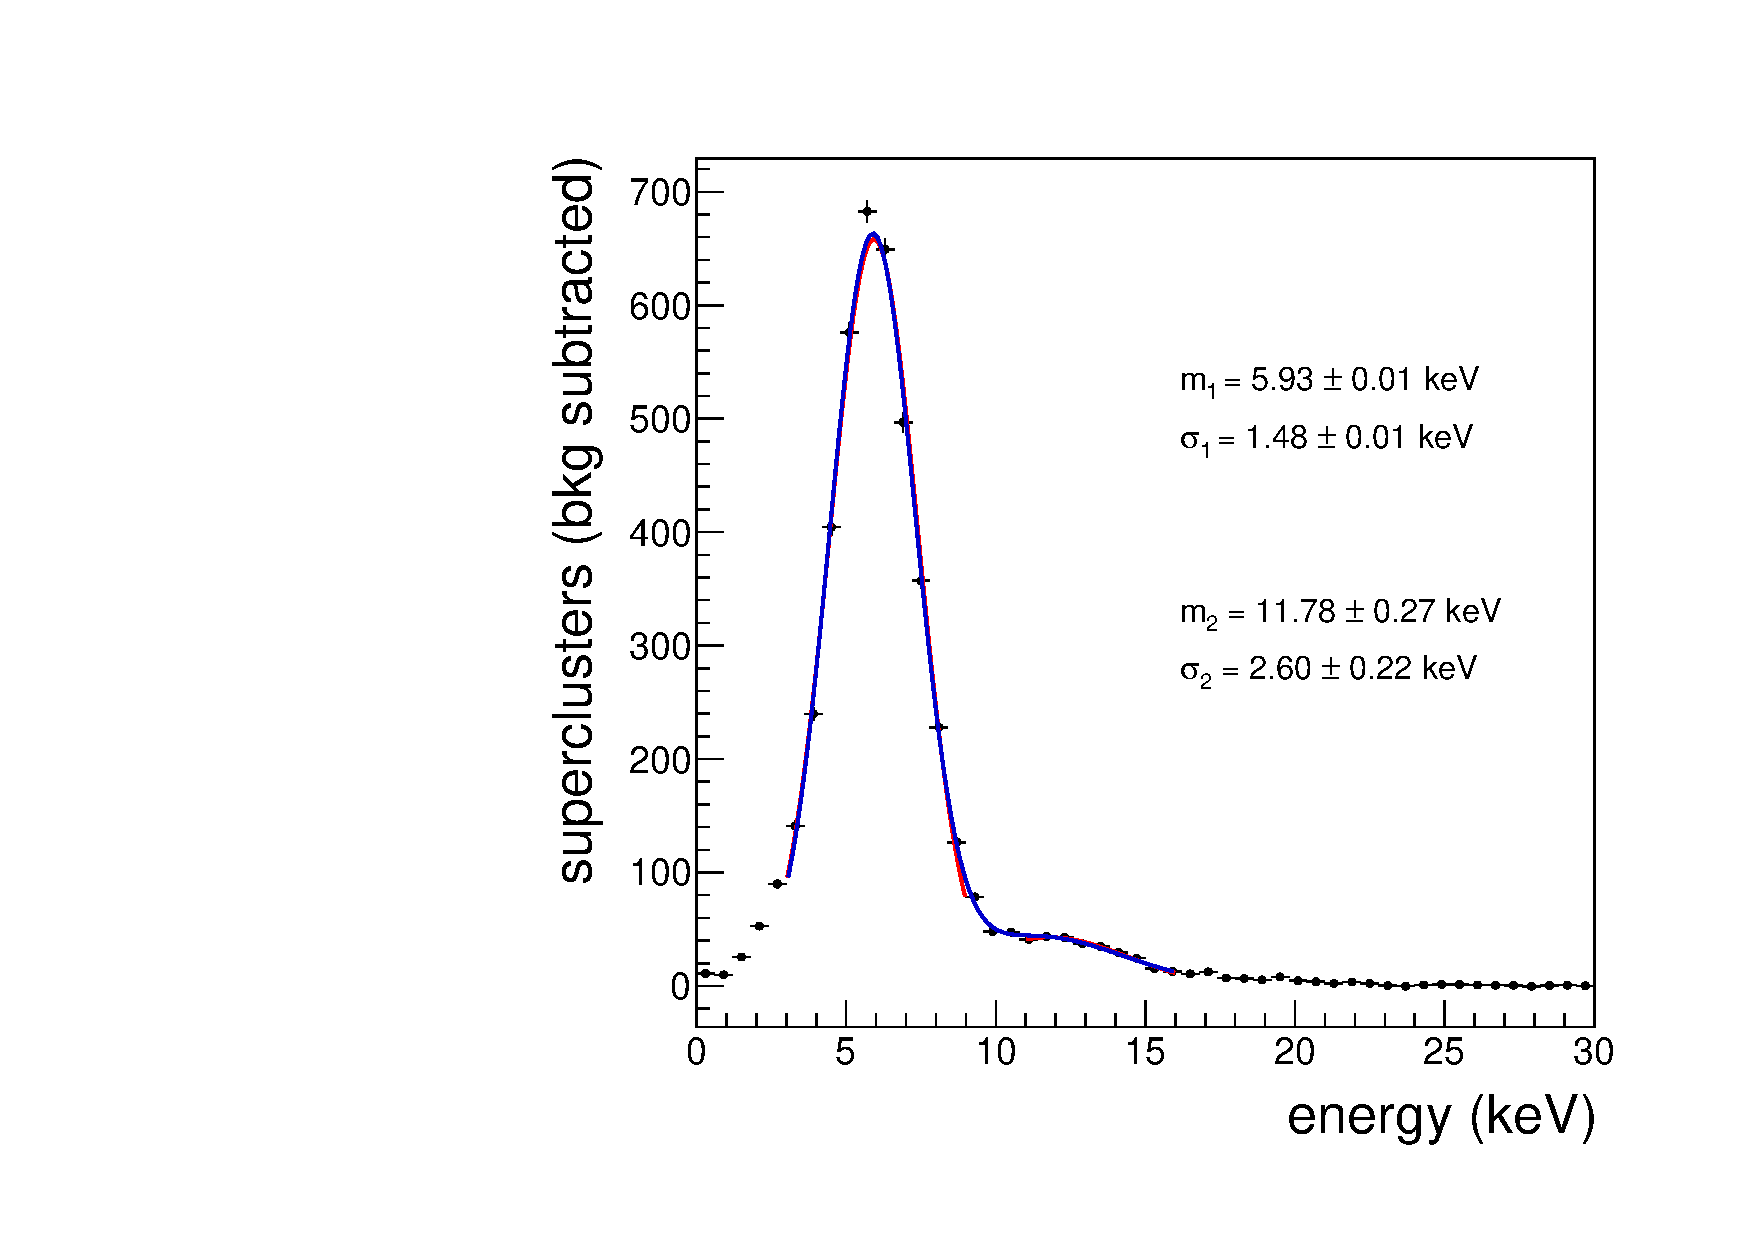
\includegraphics[width=0.49\linewidth]{figures/fe_energy_fit}
%%     \caption{Distribution of the supercluster energy, calibrated with
%%       the procedure described in the text, in events with the \fe
%%       source. Clearly visible is the large peak of a single spot, and,
%%       at around twice the energy, a broader peak for the case of two
%%       neighbor spots merged in a single supercluster.
%%       \label{fig:fepeak}}
%%   \end{center}
%% \end{figure}
%

The skeletonization procedure provides a general method to estimate
the track length ($l_p$), which is accurate both in the case of straight
and curving track.  In the case of straight tracks, the length extracted
in this way coincides with the major axis estimated with a principal
component analysis (PCA), described in the following section. For
exactly round spots, the skeleton would collapse in the center of the
cluster and the resulting length would be 1 pixel, but this completely
symmetric case never happens in the considered samples.



\section{Cluster shape observables}
\label{sec:clustershapes}
The interaction of different particles with the nuclei or the
electrons in the gas of the TPC produces different patterns of the 2D
projection of the initial 3D particle trajectory.  These
characteristics, to which we refer generically as \textit{cluster
shapes observables}, are useful to discriminate different ionizing
particles. In particular, they were used to select a pure sample of
nuclear recoil candidates produced by the interaction of the neutrons
originating from the \ambe source and to identify various sources of
backgrounds. The main cluster shape observables are described in the
following:

\begin{itemize}
  \item \textit{projected length and width:~} a SVD on the $x \times
    y$ matrix of the pixels belonging to the supercluster is
    performed. The eigenvectors found can be interpreted as the
    directions of the two axes of an ellipse in 2D. The eigenvalues
    represent the magnitudes of its semiaxes: the major one is defined
    as \textit{length}, $l$ the minor one as \textit{width},
    $w$. These are well defined for elliptic clusters, or for long and
    straight tracks. The directions along the major and the minor axis
    are defined as \textit{longitudinal} and \textit{transverse} in
    the following. The longitudinal and transverse supercluster
    profiles, for the cosmic ray track candidates shown as an example
    in Fig.~\ref{fig:super_clusters2} (bottom) are shown in
    Fig.~\ref{fig:profiles}. The longitudinal profile shows the
    typical pattern of energy depositions in clusters, while the
    transverse profile, dominated by the diffusion in the gas, shows a
    Gaussian shape. It has to be noted that the cluster sizes
    represent only the projection of the 3D track in the TPC on the 2D
    $x$--$y$ plane;

    \begin{figure}[ht]
      \begin{center}
        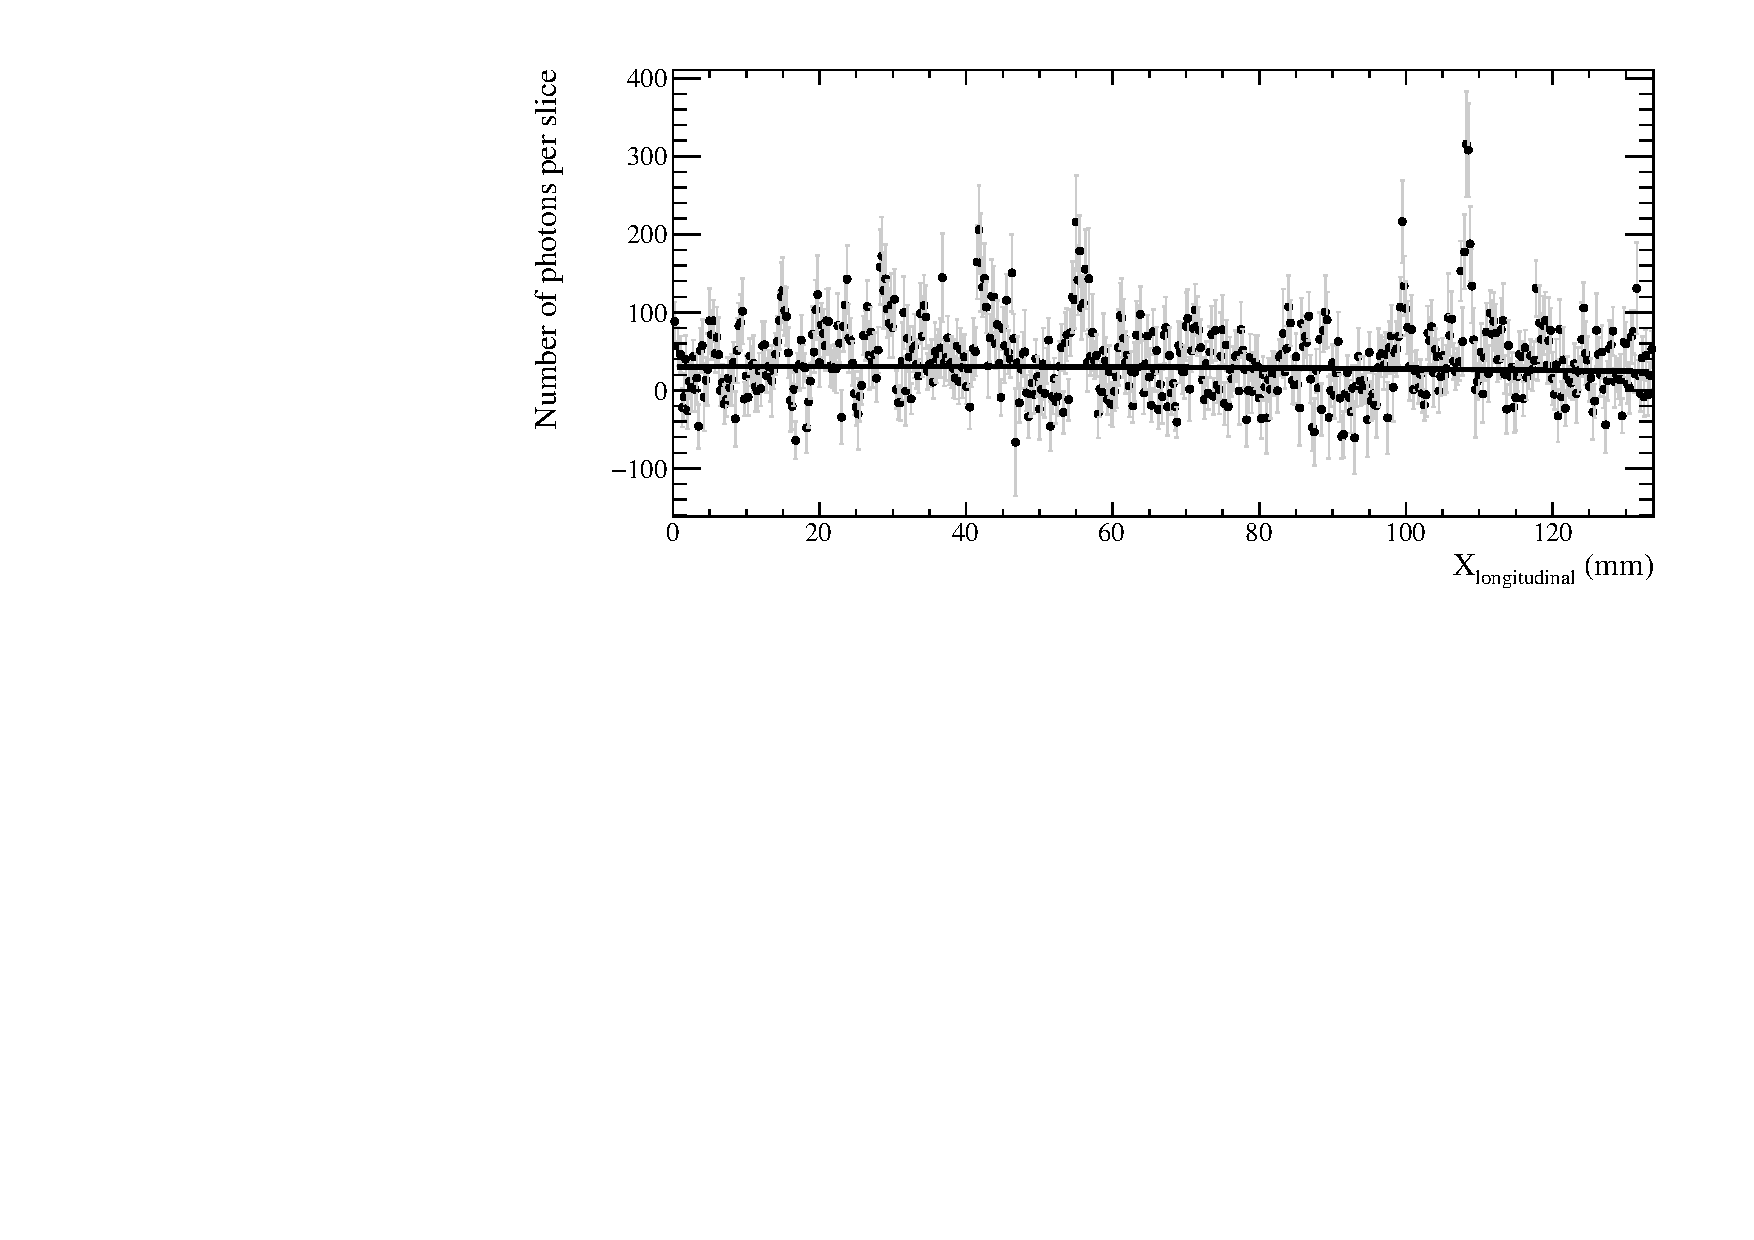
\includegraphics[width=0.45\linewidth]{figures/pic_run02156_ev631_cluster1_longprofile}
        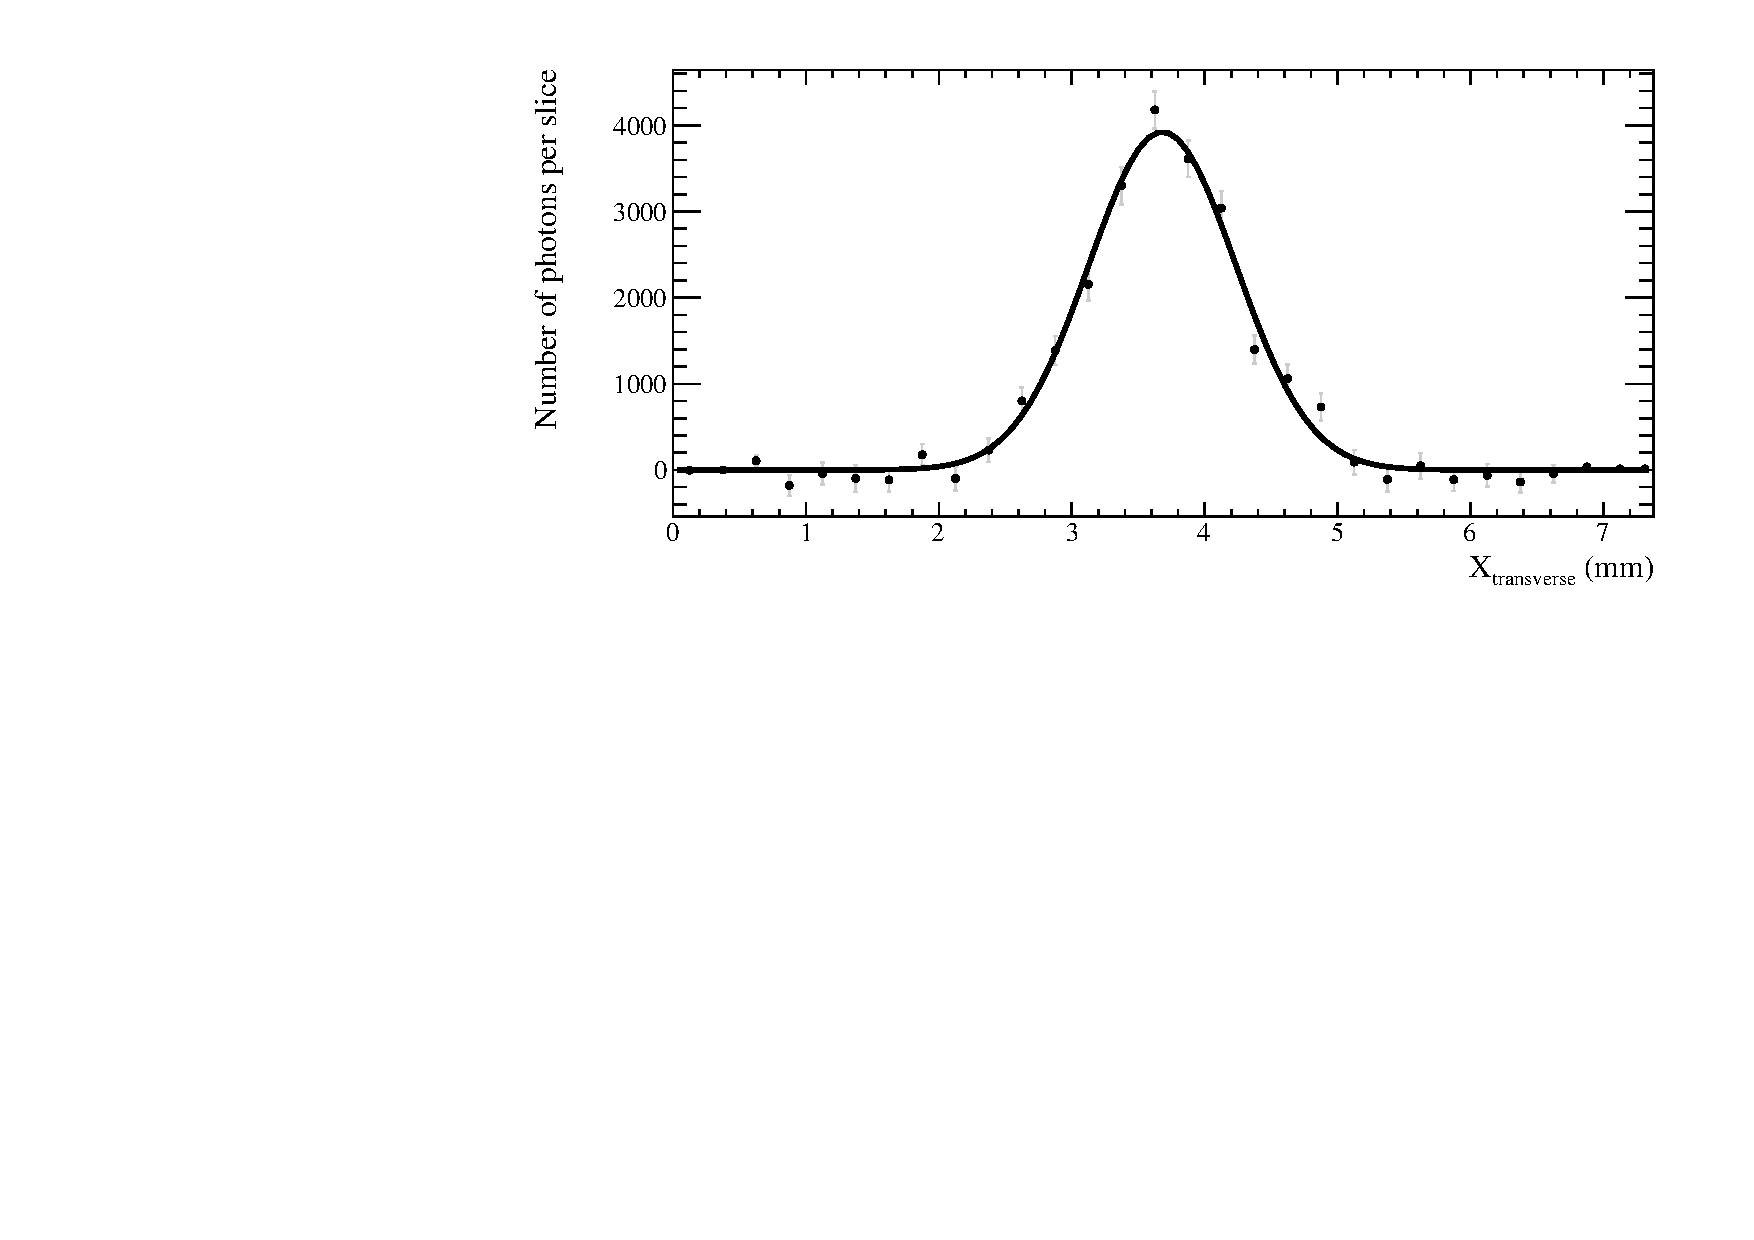
\includegraphics[width=0.45\linewidth]{figures/pic_run02156_ev631_cluster1_latprofile}
        \caption{Supercluster profile in the longitudinal (top) or
          transverse (bottom) direction, for a long and straight
          cosmic ray track candidate shown in  Fig.~\ref{fig:super_clusters2} (bottom). The longitudinal profile shows an
          energy deposition in sub-clusters, while the transverse
          direction shows the typical width of the diffusion in the
          gas. For the longitudinal profile, the line represent the
          average number of photons per slice. For the transverse
          profile, it represents a fit with a Gaussian
          PDF. \label{fig:profiles}}
      \end{center}
    \end{figure}

  \item \textit{projected path length:~} for curly and kinky tracks
    the values returned by the SVD of the supercluster are not an
    accurate estimates of their size. While the width is dominated by
    the diffusion, the length for patterns like the one shown in the
    example of Fig.~\ref{fig:super_clusters1} is ill-defined. Thus,
    the more general path length, $l_p$, computed with the
    skeletonization procedure in Fig.~\ref{fig:skeleton} is used to
    estimate the linear extent for both straight and curved tracks.

  \item \textit{Gaussian width:~} the original width of the track in
    the transverse direction is expected to be much lower than the
    observed width induced by the diffusion in the gas. Thus, as shown
    in Fig.~\ref{fig:profiles} (right), the standard
    deviation, \tsigmag, can estimated by a fit with a Gaussian
    probability density function (PDF);

  \item \textit{slimness:~} the ratio of the width over the path
    length, $\xi=w/l_p$, represents the aspect ratio of the
    cluster. It is very useful to discriminate between cosmic
    rays-induced background (long and thin) from low energy nuclear or
    electron recoils (more elliptical or round, as the \fe spots);
    
  \item \textit{integral:~} the total number of photons detected by all the
  pixels gathered in the supercluster, \isclu, as defined in
  Eq.~\ref{eq:integral};

  \item \textit{pixels over threshold:~} the number of pixels in the
  supercluster passing the zero-suppression threshold, $n_p$;

  \item \textit{density:~} the ratio $\delta$ of \isclu, divided by
  $n_p$, as defined in Eq.~\ref{eq:density};

  \item \textit{energy:~} the calibrated energy, expressed in keV. The
    calibration method simultaneously performs both the per-slice
    correction as a function of the local $\delta$, and the absolute
    energy scale calibration, which corrects the non perfect
    containment of the cluster, \ie, the bias in the distribution of
    $E/E_{true}$, using with \fe source.
\end{itemize}

The projected supercluster path length, $l_p$, and Gaussian transverse
size, \tsigmag, are shown in Fig.~\ref{fig:clsize}, for data taken in
different types of runs.  During the data-taking approximately 3000
frames were recorded in absence of any external radioactive source
({\it no-source} sample). In these frames the interaction of
ultra-relativistic cosmic ray particles (mostly muons) are clearly
visible as very long clusters. Internal radioactivity of the \lemon
materials also contribute with several smaller size clusters. About
1500 frames were acquired with the \ambe source, and approximately
$10^4$ calibration images with \fe source. In Fig.~\ref{fig:clsize},
as well as in the following ones showing other cluster properties, the
distributions obtained in runs without radioactive sources are
normalized to the \ambe data total CMOS exposure time. For the data
with \fe source, since the activity of the source is such to produce
about 15 clusters/event, the data are scaled by a factor one-tenth
with respect to the \ambe exposure time for clearness. Considerations
about the trigger efficiency scale factor between data with and
without an radioactive source are detailed later. The distributions in
this section aim to show the different cluster shape observables among
the different kinds of events.

\begin{figure}[ht]
  \begin{center}
  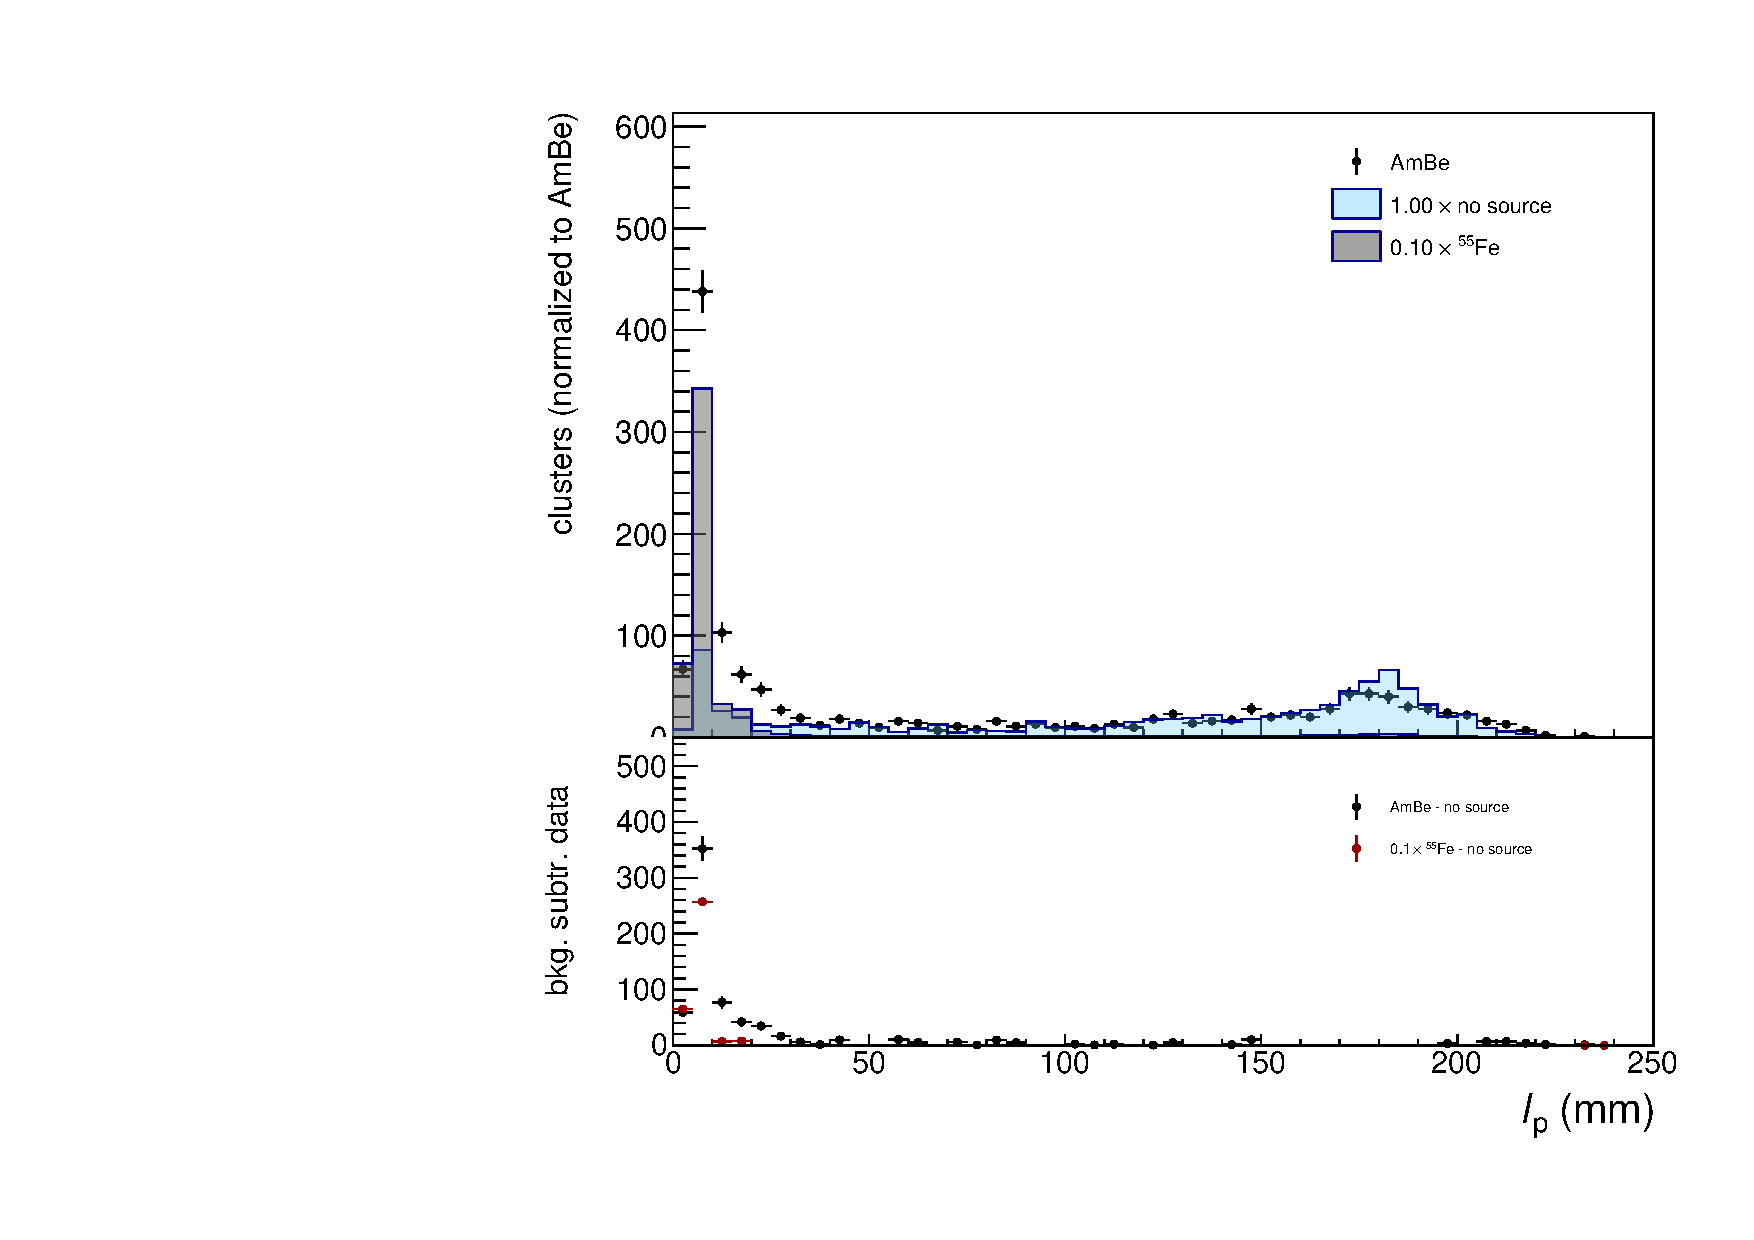
\includegraphics[width=0.45\linewidth]{figures/length}
  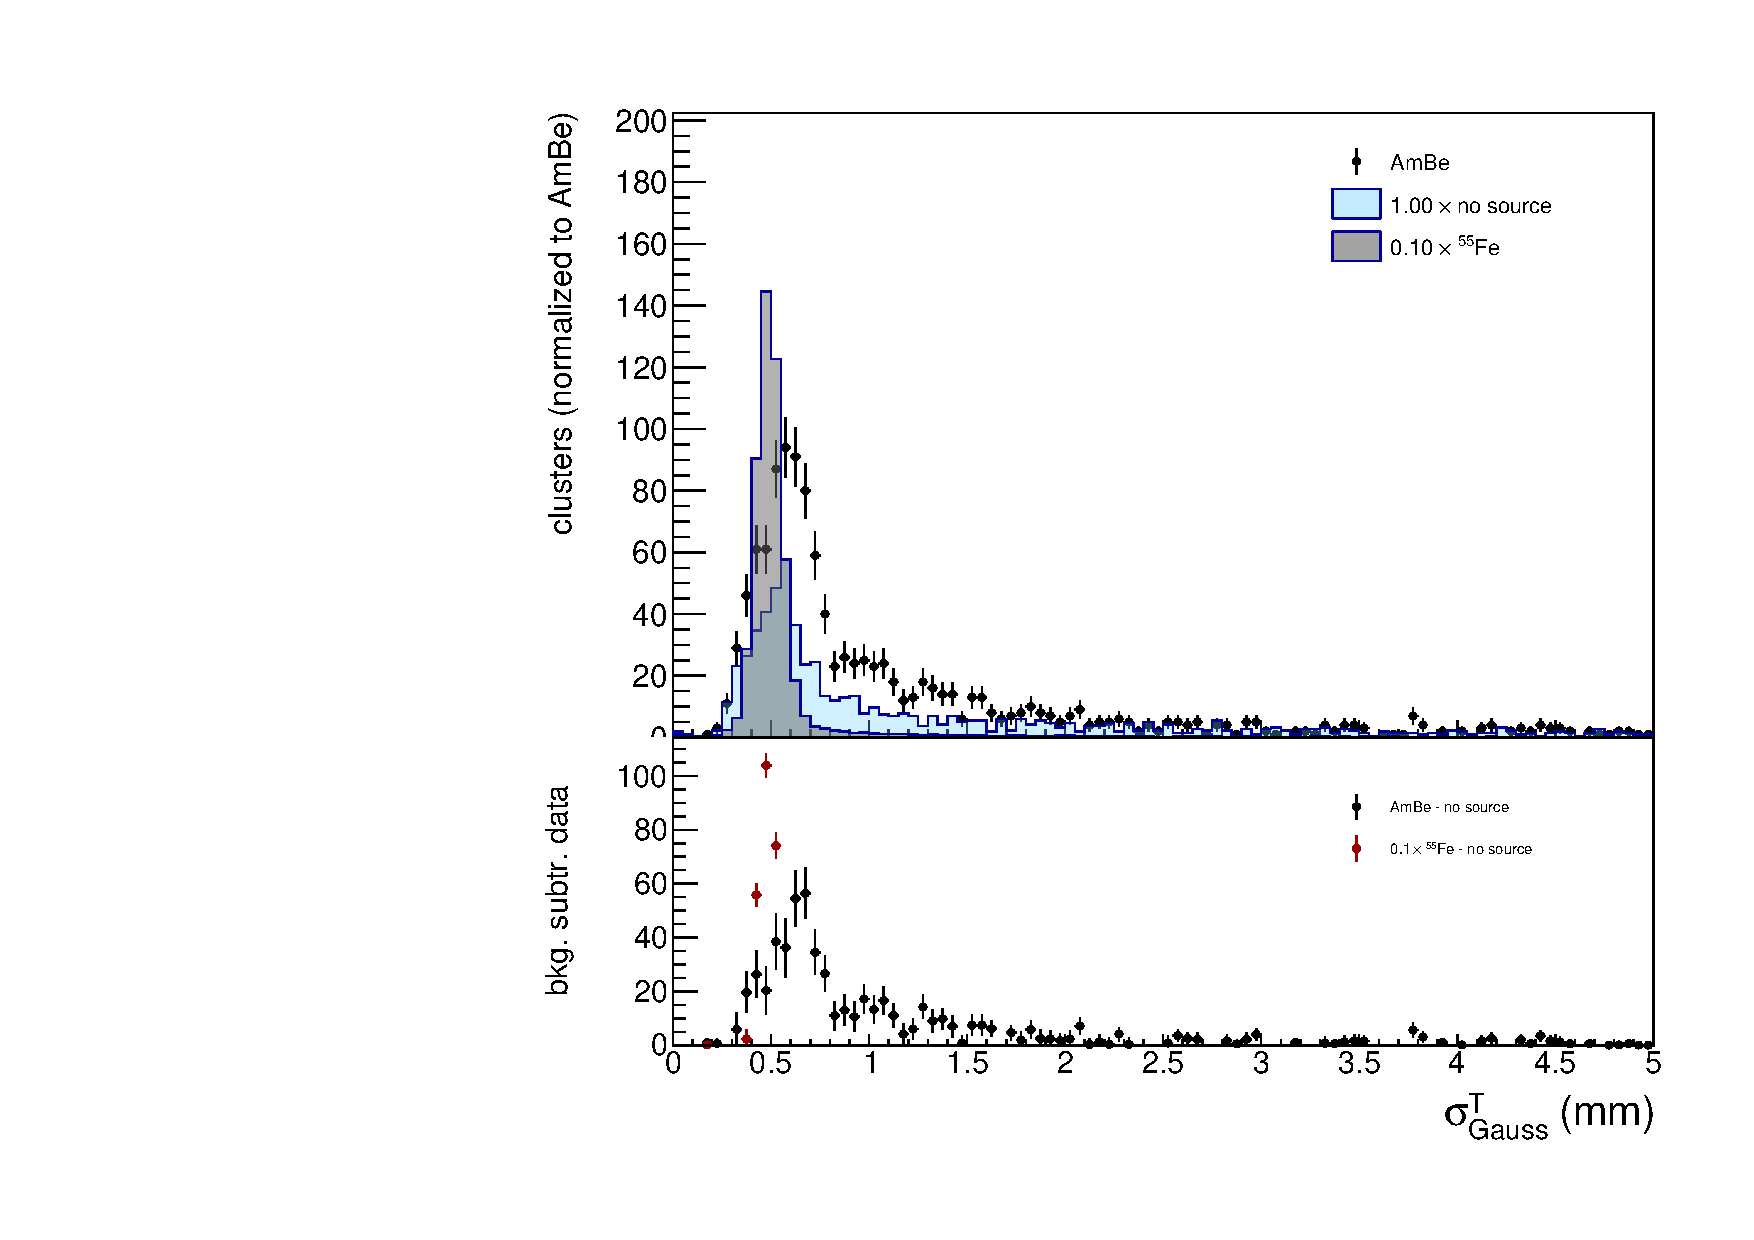
\includegraphics[width=0.45\linewidth]{figures/tgausssigma}

  \caption{Supercluster sizes projected onto the $x$--$y$ plane. Left:
    longitudinal path length, $l_p$.  Right: transverse Gaussian
    spread, \tsigmag. Filled points represent data with \ambe source,
    dark gray (light blue) distribution represents data with \fe
    source (no source).  The normalization of data without any
    radioactive source is scaled to the same exposure time of
    the \ambe one. For the data with \fe source , a scaling factor of
    one tenth is applied for clearness, given the larger activity of
    this source.  \label{fig:clsize}}

    \end{center}
\end{figure}

Figure~\ref{fig:clsize} shows the cluster sizes distributions in the
longitudinal and transverse directions for different sets of
runs. Data show an average Gaussian width for the \fe spots
$\tsigmag\approx500$\unit{$\mu$m} (dominated by the diffusion in the
gas), while it is larger, approximately 625\unit{$\mu$m}, for data
with \ambe source.  The contribution of cosmic rays, present in all
the data, is clearly visible in the data without any radioactive
source, corresponding to clusters with a length similar to the
detector transverse size (22\unit{cm}).

Other observables are the slimness, $\xi$, and the light density,
$\delta$, shown in Fig.~\ref{fig:clshape}. The former is a useful
handle to reject tracks from cosmic rays, which typically have a slim
aspect ratio, \ie, low values of $\xi$, while the clusters from \fe
are almost round, with values $0.9\lesssim\xi<1$. By construction,
$\xi<1$, since the width is computed along the minor axis of the
cluster, and for round spots it peaks at around 0.9. The apparent
threshold effect is purely geometrical, due to the minimal size of the
macro-pixel ($4{\times}4$) used at the basic clustering step which can
be larger than a round spot from \fe. Data with \ambe source, which
contains a component of nuclear recoils, show a component of round
spots, similar in size to the ones of \fe, and a more elliptical
component, with $0.4<\xi<0.8$ values. Finally, the light density,
$\delta$, is the variable expected to better discriminate among
different candidates: cosmic rays induced background, electron recoils
and nuclear recoil candidates. This is the variable used in this paper
for the final particle identification. The identification results can
be improved using additional cluster shape variables, also profiting
of their different correlations for signal and background clusters,
via a multivariate approach, but here priority is given to the
straightforwardness, rather than the ultimate performance.

\begin{figure}[ht]
  \begin{center}
  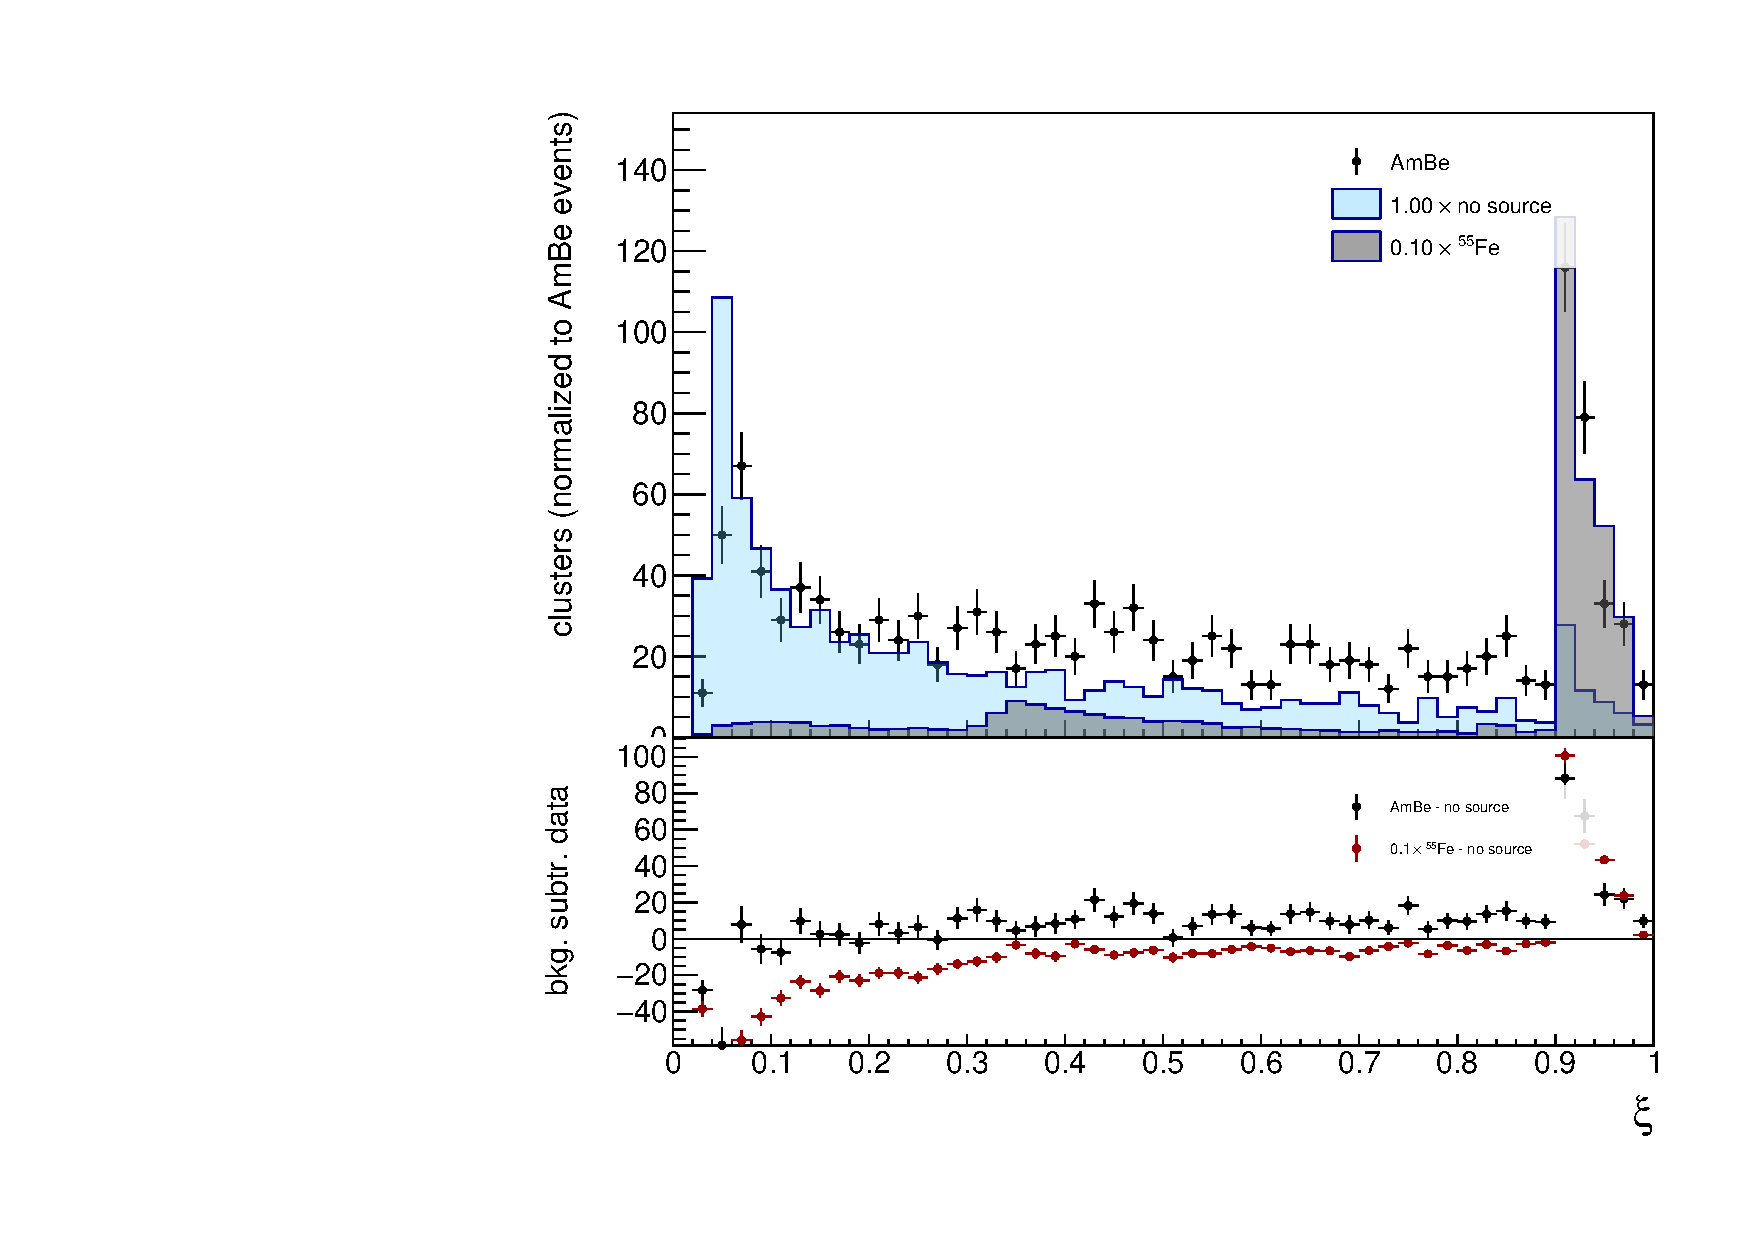
\includegraphics[width=0.45\linewidth]{figures/slimness}
  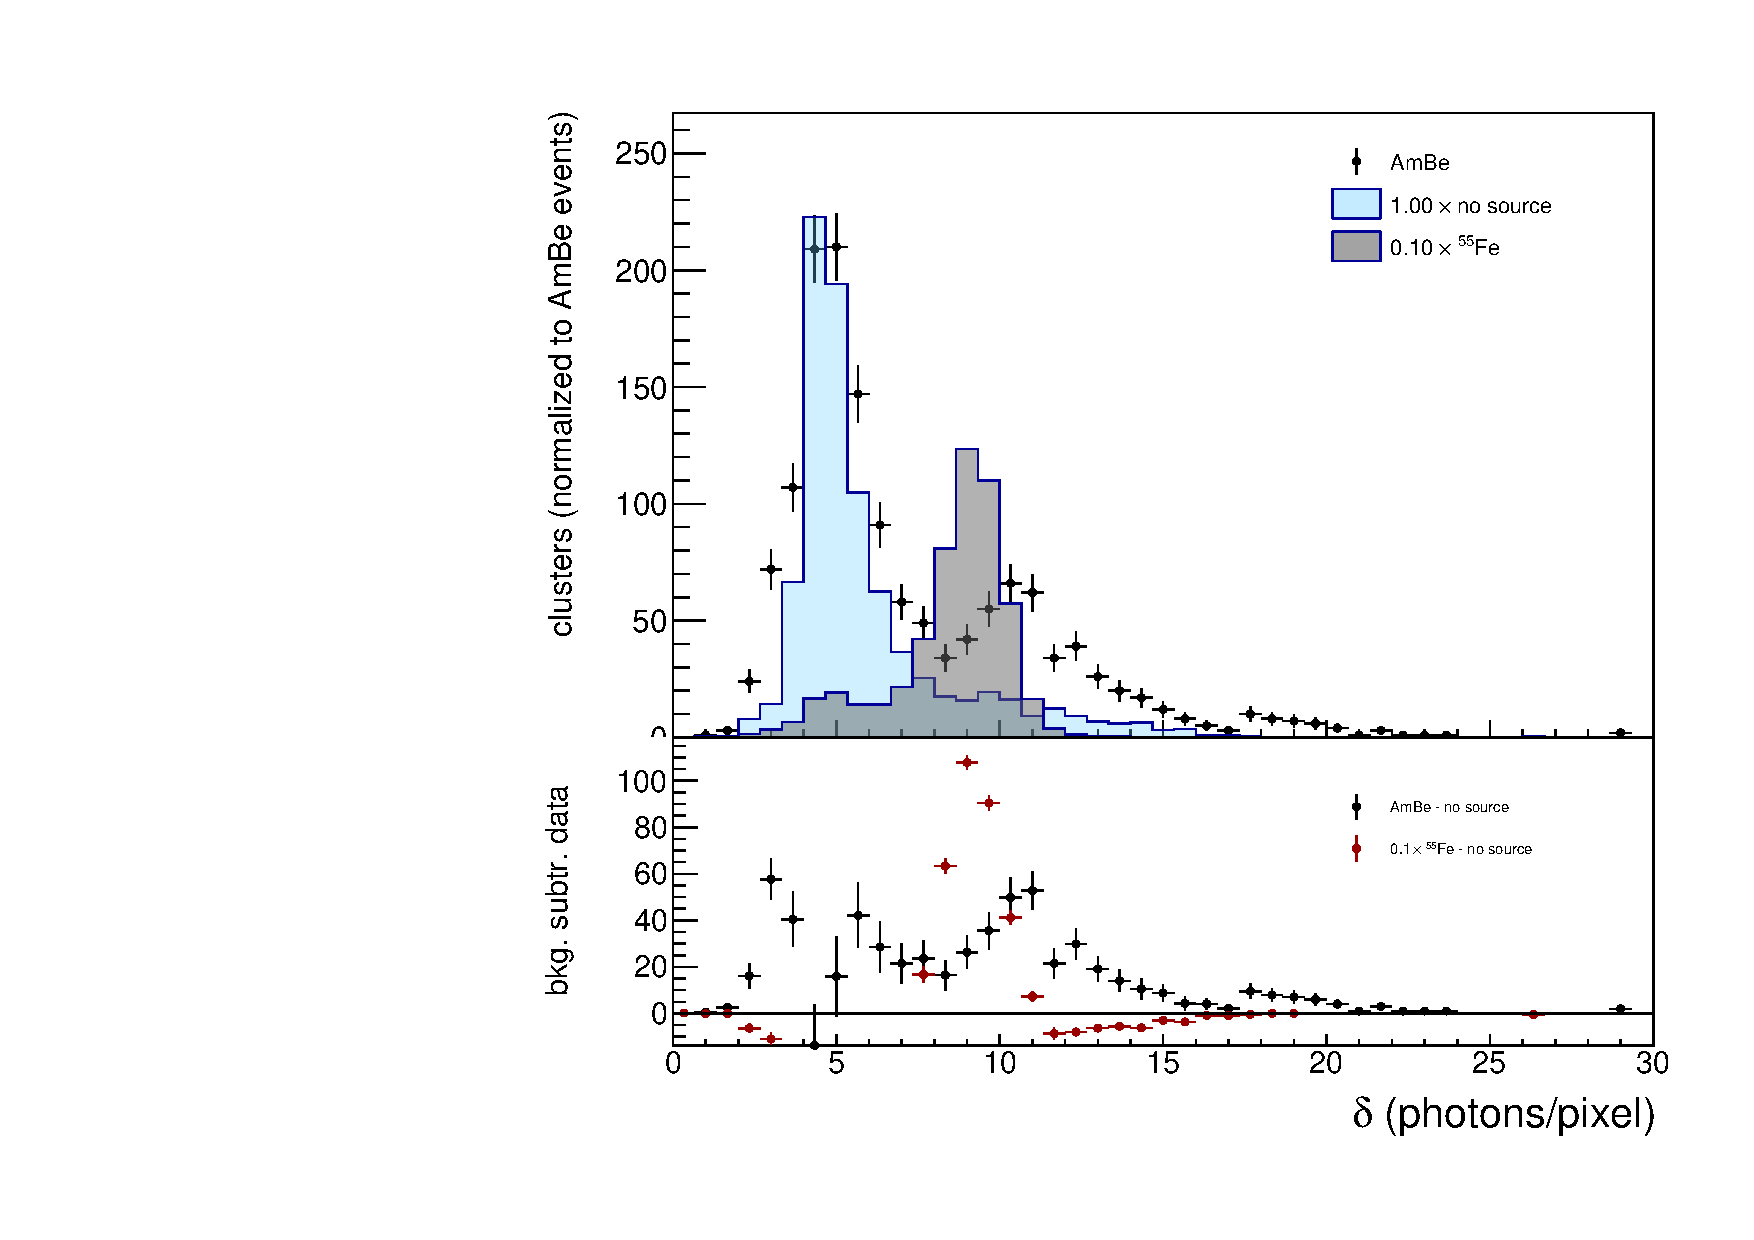
\includegraphics[width=0.45\linewidth]{figures/density}

  \caption{Supercluster variables. Left: slimness $\xi$; right: light
    density $\delta$. Filled points represent data with \ambe source,
    dark gray (light blue) distribution represents data with \fe
    source (no source).  The normalization of data without source is
    to the same exposure time of the \ambe one. For the data with \fe,
    a scaling factor of one tenth is applied for clearness, given the
    larger activity of this source. \label{fig:clshape}}

\end{center}
\end{figure}

Finally, Fig.~\ref{fig:energy} (left) shows the calibrated energy
($E$) spectrum for the reconstructed superclusters. The energy
spectrum shows the $E=5.9\keV$ peak in the first bin of the
distribution for data with \fe source, and the expected broad peak for
minimum ionizing particles traversing the $\approx$20\unit{cm} gas
volume at around 60\keV. The distribution of the observed average
projected \dedl for the no-source sample and for the \ambe samples is
shown in Fig.~\ref{fig:energy} (right). The broadening of the
distribution is mainly due to the specific energy loss fluctuation in
the gas mixture of the cosmic ray particles.  Its modal value,
corrected for the effect of the angular distribution (an average
inclination of 56$^{\circ}$ was measured from track reconstruction) is
2.5\keV/cm, in good agreement with the \garfield prediction of
2.3\keV/cm.

\begin{figure}[ht]
  \begin{center}
  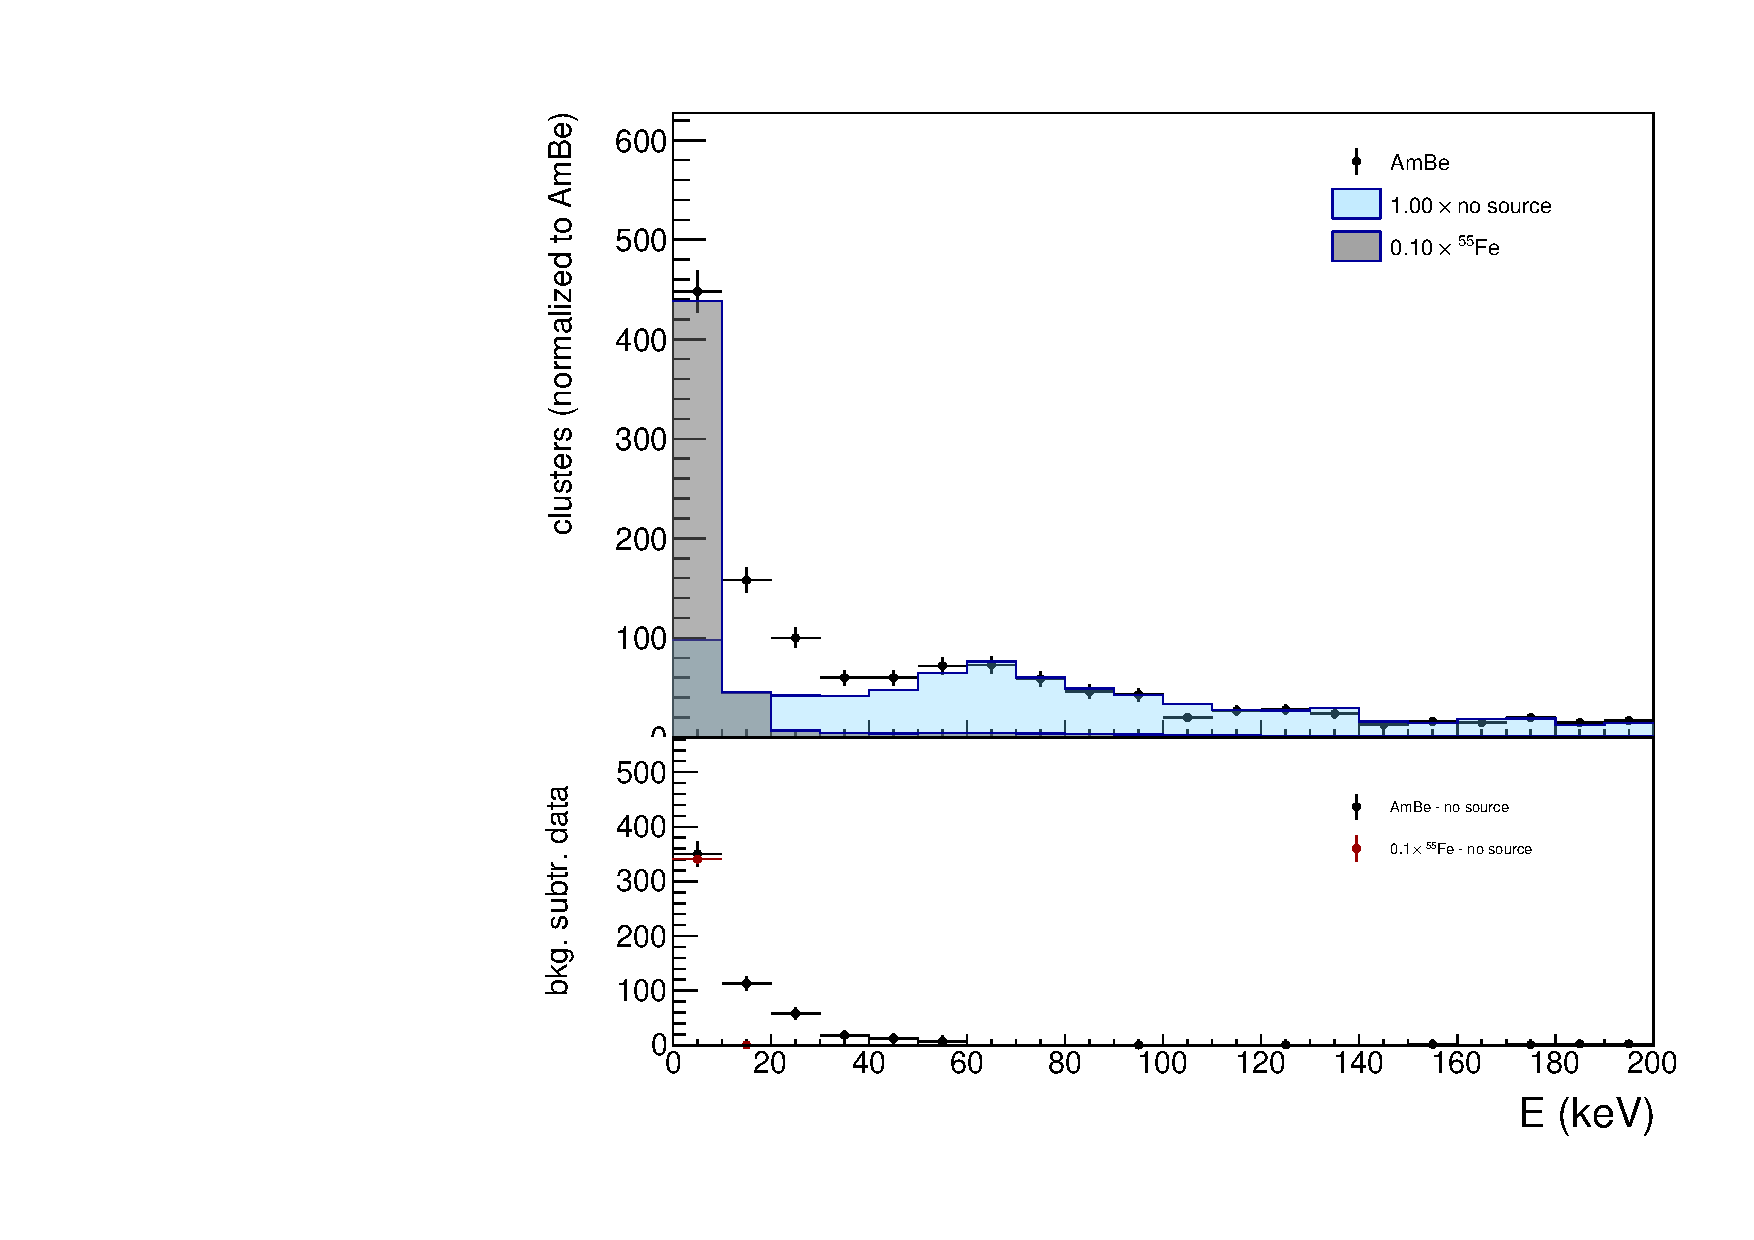
\includegraphics[width=0.45\linewidth]{figures/energyExt}
  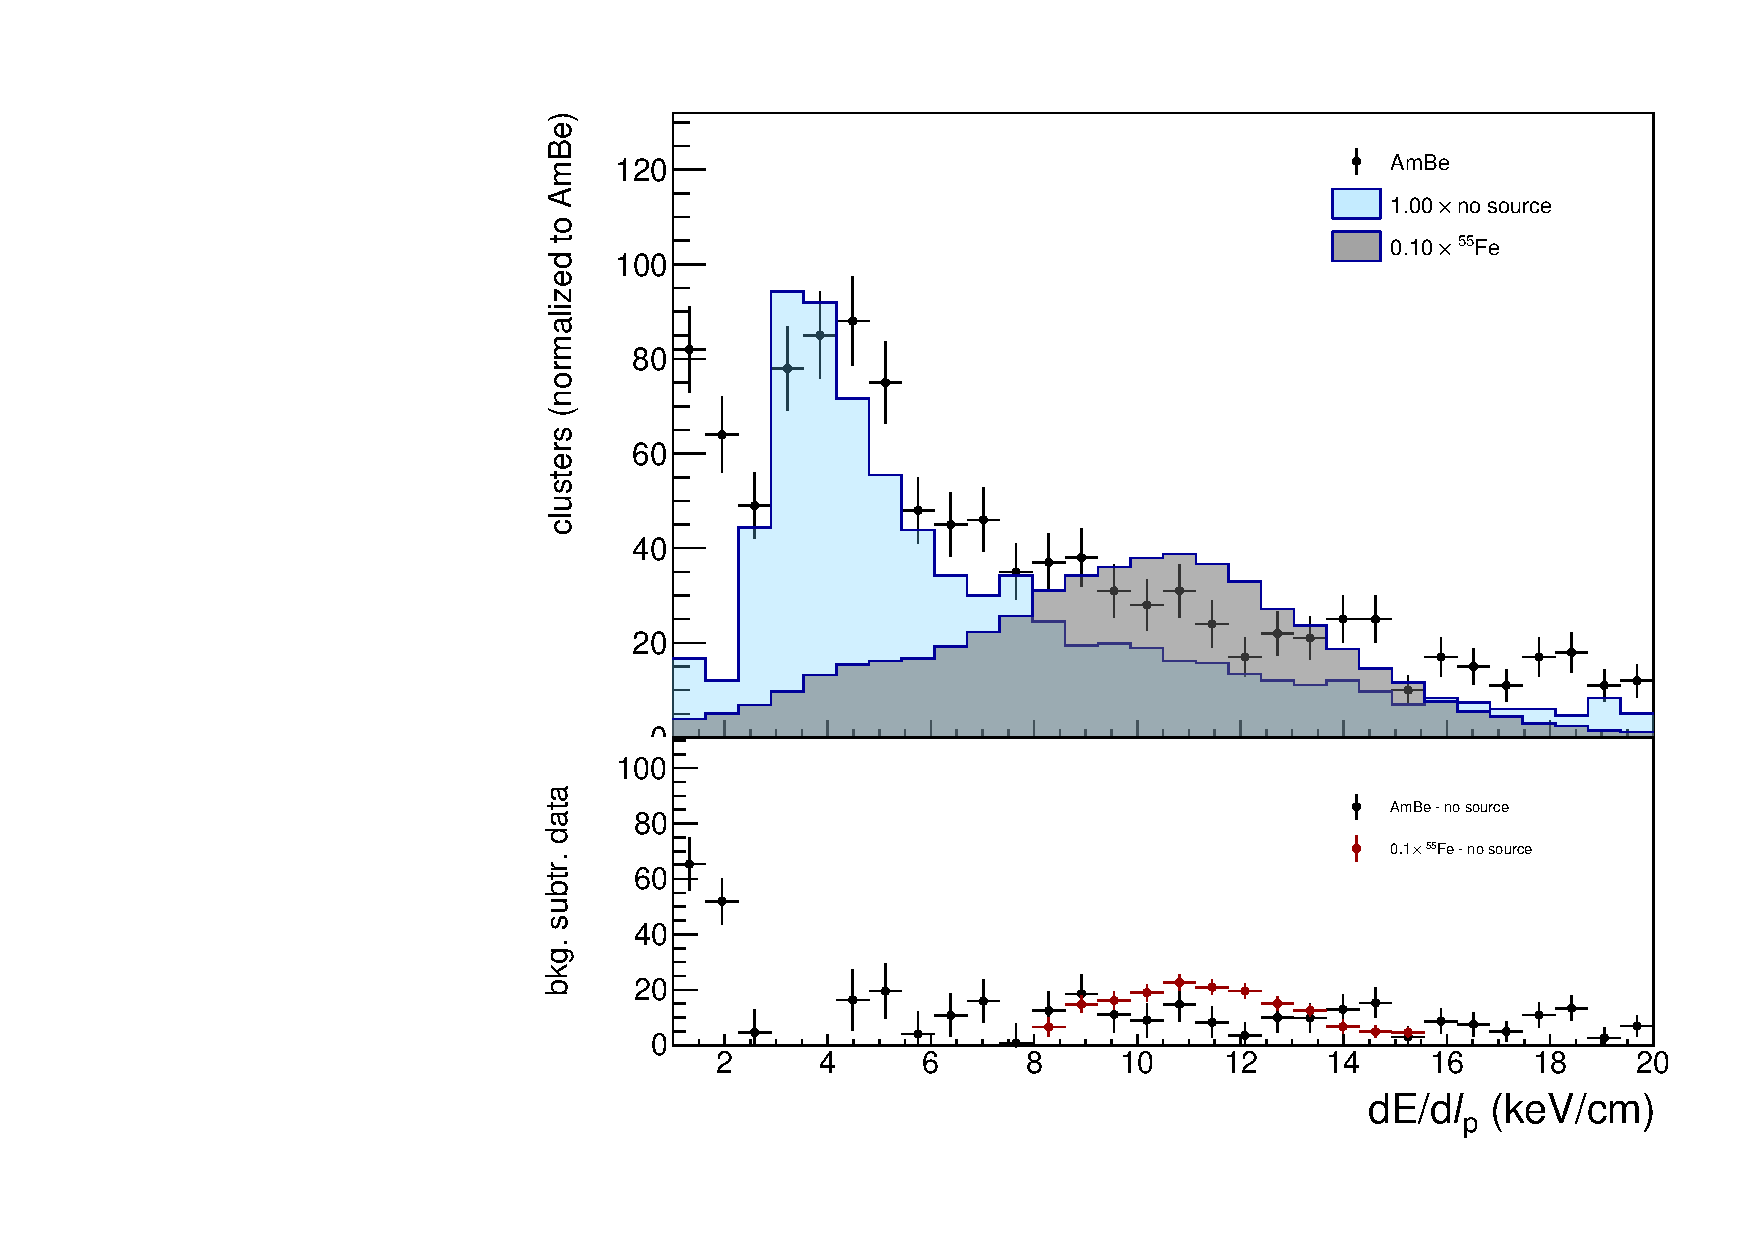
\includegraphics[width=0.45\linewidth]{figures/dedx}

  \caption{Supercluster calibrated energy spectrum (left) and their
    average \dedl. Filled points represent data with \ambe source,
    dark gray (light blue) distribution represents data with \fe
    source (no source).  The normalization of data without source is
    to the same exposure time of the \ambe one. For the data with \fe,
    a scaling factor of one tenth is applied for clearness, given the
    larger activity of this source. \label{fig:energy}}

\end{center}
\end{figure}

\subsection{Background normalization}
\label{sec:background}
The data with \ambe source, taken on the Earth surface, suffers from a
large contribution of interactions of cosmic rays, and from ambient
radioactivity, whose suppression is not optimized for the \lemon
detector. The cluster shape observables provide a powerful handle to
discriminate them from nuclear recoils candidates, but the small
residual background needs to be statistically subtracted. The
distributions shown earlier, where the different types of data are
normalized to the same exposure time, demonstrate that the live-time
normalization provides already a good estimate of the amount of cosmic
rays in data with radioactive sources. This approach does not account
for a possible bias from the trigger, which is generated by the PMT
signals, as described in Sec.~\ref{sec:layout}. Indeed, in runs with
the \ambe source, the PMT can trigger both on signals from neutron
recoils or photons produced by the $^{241}$Am, and on ubiquitous
signals from cosmic rays, while in the sample without source only the
latter are possible.  Therefore, during the same exposure time,
the probability to trigger on cosmic rays is lower in events
with \ambe than in no-source events. The trigger efficiency scale
factor, $\varepsilon_{SF}$, can be obtained as the ratio of the number
of clusters selected in pure control samples of cosmic rays ($CR$)
obtained on both types of runs:
\begin{equation}
\label{eq:sfeff}
\varepsilon_{SF} = \frac{N^{AmBe}_{CR}}{N^{no-source}_{CR}}.
\end{equation}

The $CR$ control region is defined by selecting clusters with
$l>13$\unit{cm}, $\xi<0.1$, $\tsigmag<6$\unit{mm}, and having an
energy within a range dominated by the cosmic rays contribution,
$50<E<80\keV$. The selected clusters show small values of
$\delta\approx5$, well compatible with the small specific ionization
of ultra-relativistic particles.  This sample is limited in
statistics, but it is expected to be almost 100\% pure. The scale
factor obtained is $\varepsilon_{SF}=0.75\pm0.02$.

In Fig.~\ref{fig:cosmics} the typical light density and polar angle
(with respect the horizontal axis) distributions for long clusters of
any energy, still dominated by cosmic rays, are shown for the \ambe
and for the no-source sample, after having applied the
$\varepsilon_{SF}$ scale factor to the latter. Clusters with
$\delta<6$ are thus expected to be mostly coming from muon tracks, and
they show indeed a polar angle which is shifted at values towards
$90^\circ$.


\begin{figure}[ht]
  \begin{center}
  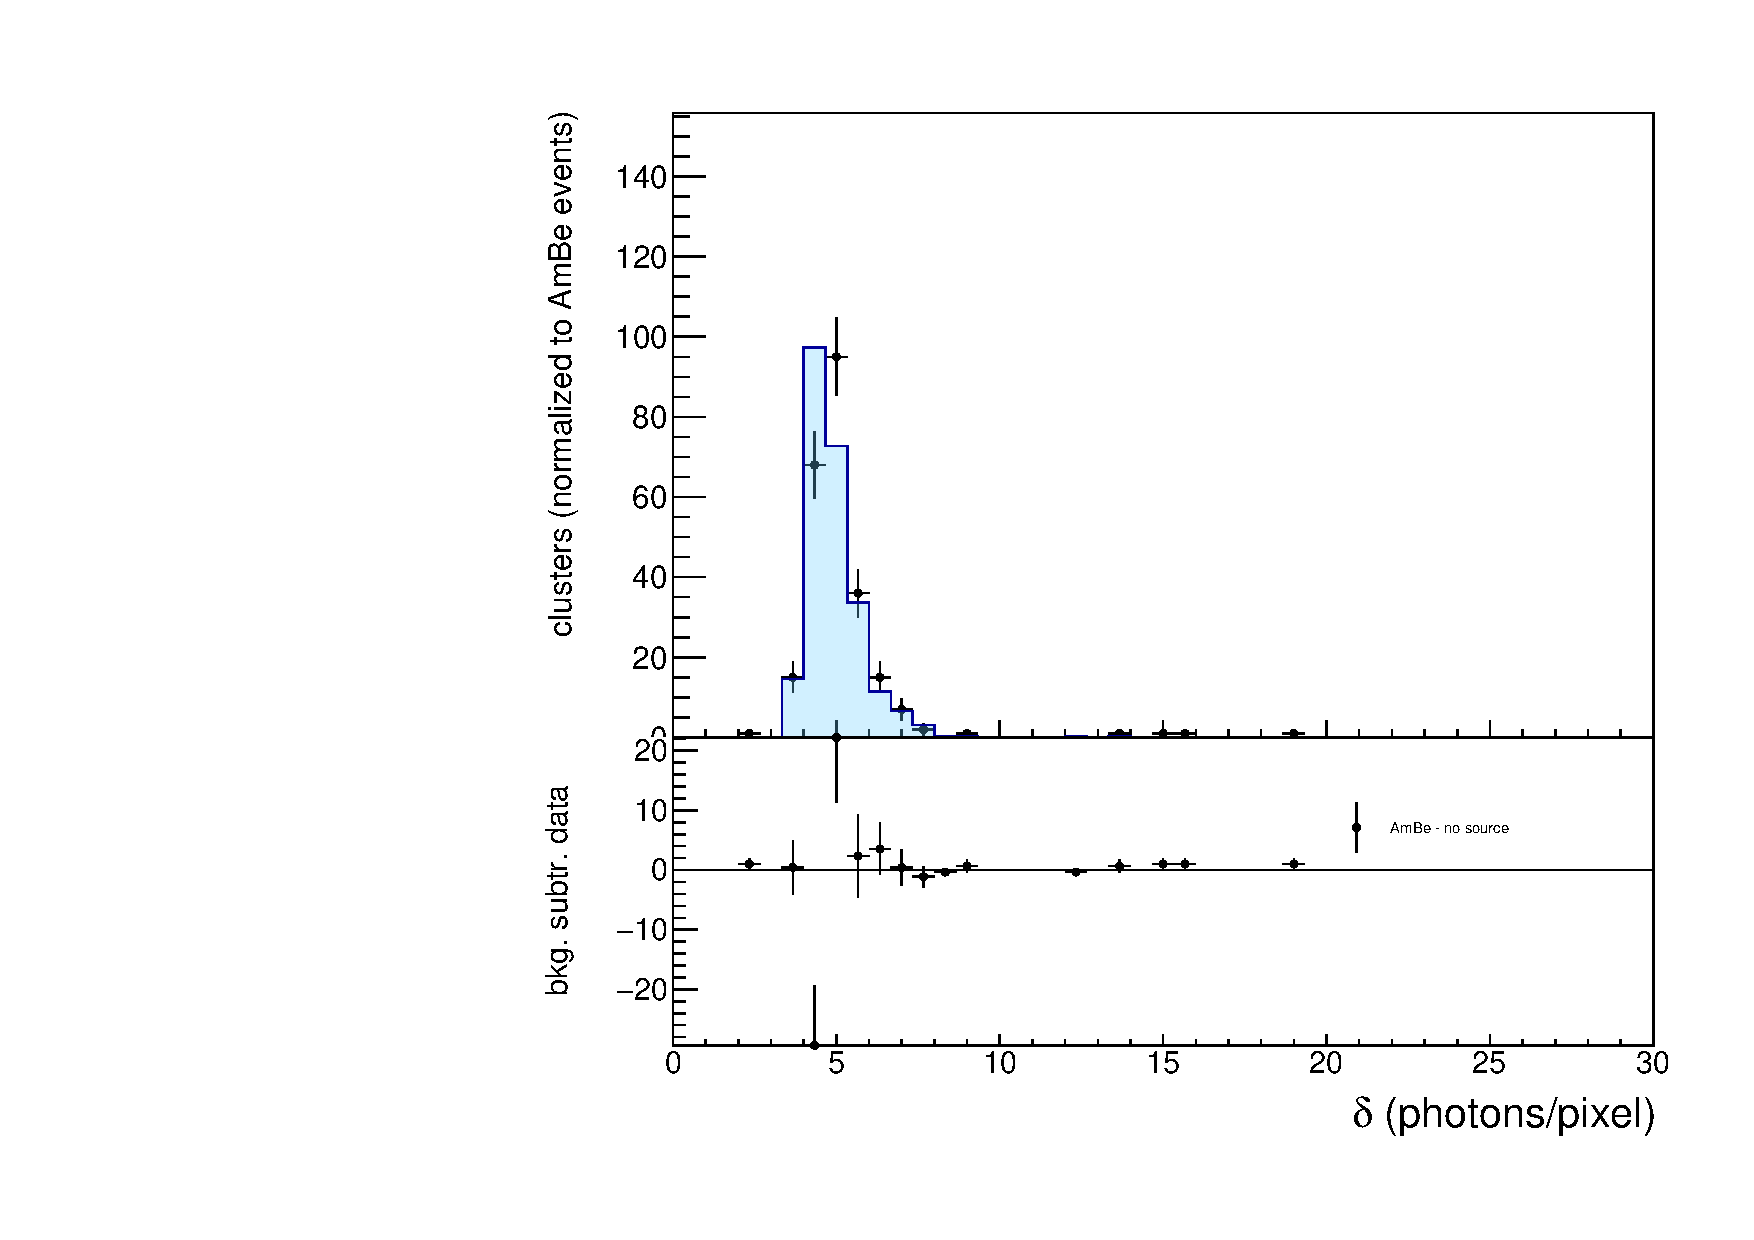
\includegraphics[width=0.45\linewidth]{figures/density_cosmics}
  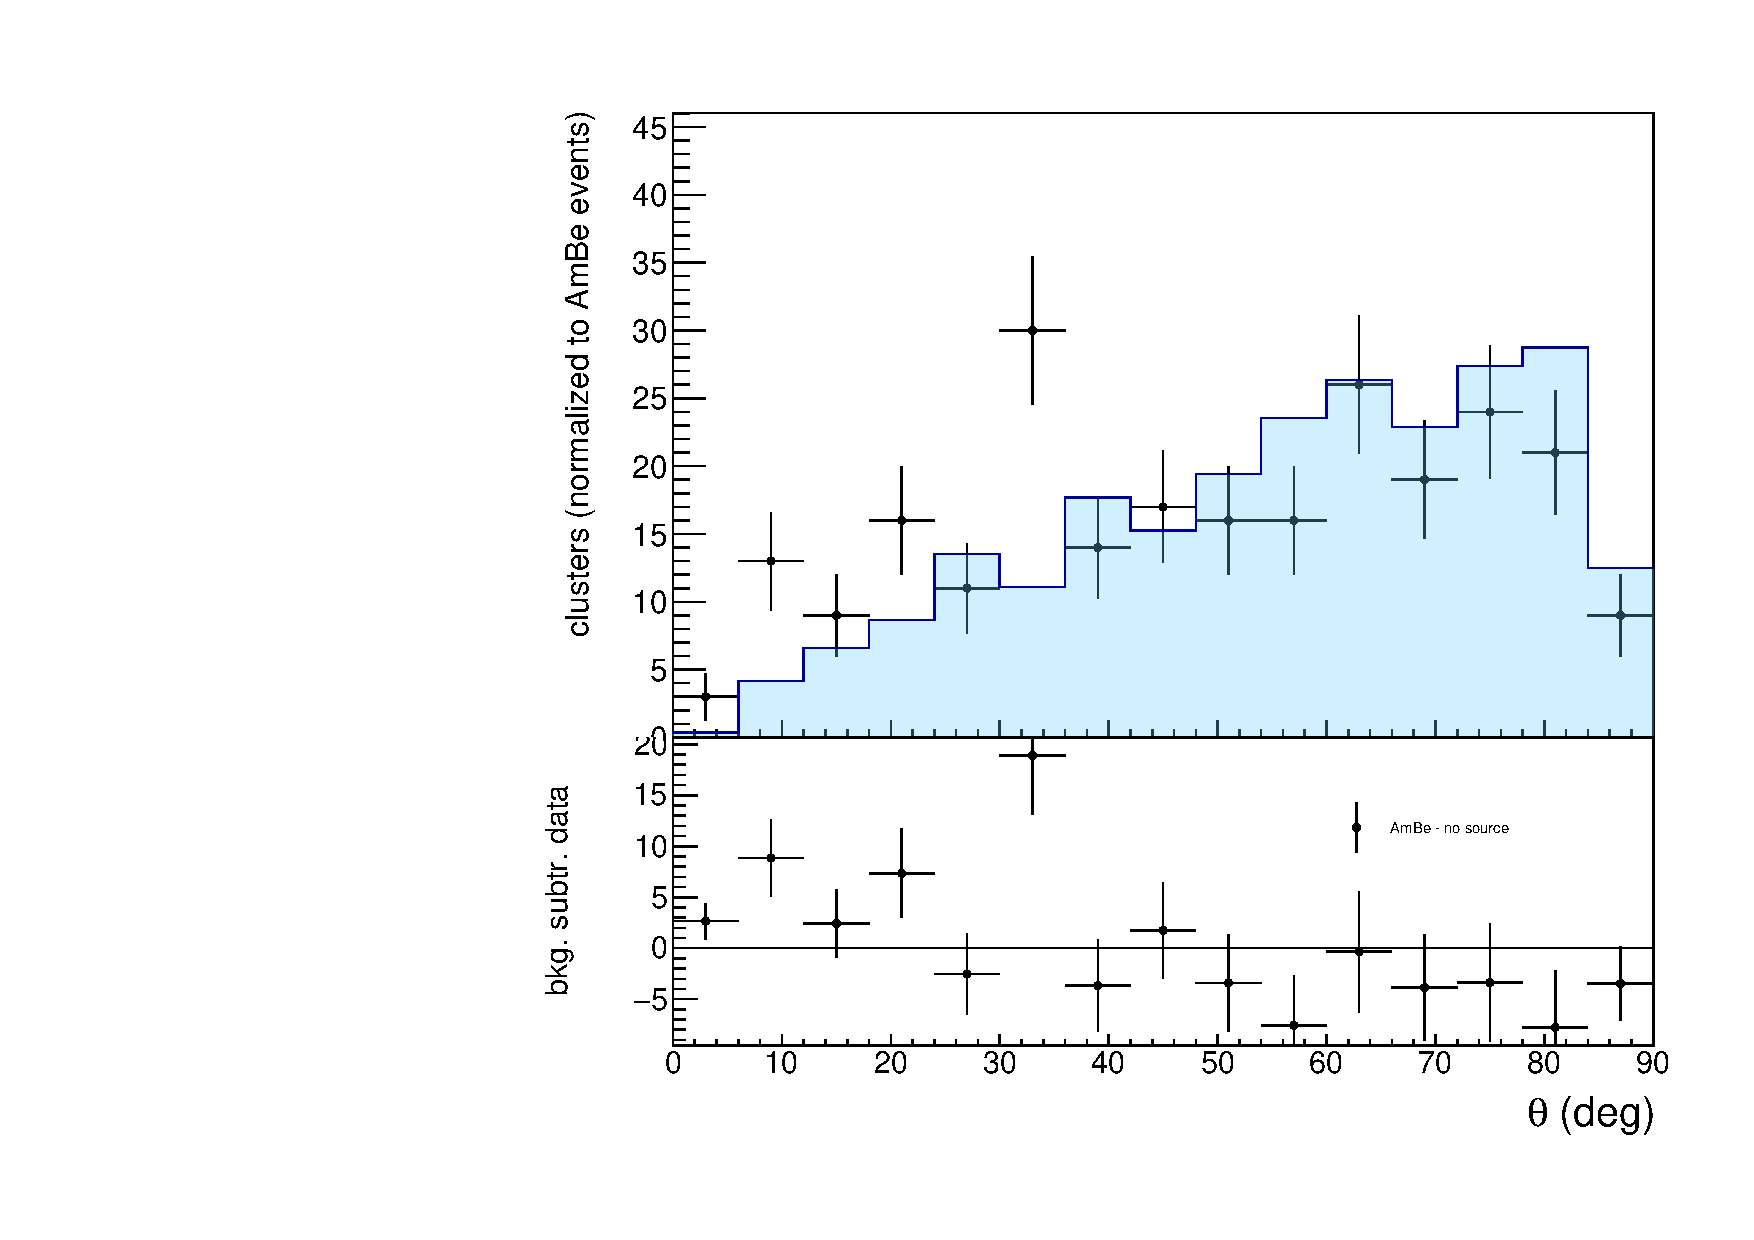
\includegraphics[width=0.45\linewidth]{figures/inclination_cosmics}

  \caption{Supercluster light density $\delta$ (left) and polar angle
    (right) - with respect the horizontal axis - distributions for
    long clusters, dominated by cosmic rays tracks.  Filled points
    represent data with \ambe source, light blue distribution
    represents data without any radioactive source.  The normalization
    of data without source is to the same exposure time of the \ambe
    one, accounting for the trigger scale factor $\varepsilon_{SF}$,
    as defined in the text.  \label{fig:cosmics}}

\end{center}
\end{figure}


 
\section{Nuclear recoil identification results}
\label{sec:results}
The main observable to distinguish the signal of nuclear recoils from
the various types of background, is the energy density $\delta$ of the
cluster.

\subsection{Signal Preselection}
To enhance the purity of the signal sample, a pre-selection was
applied, prior to a tighter selection on $\delta$: clusters with
$l_p>6.3$\unit{cm} or $\xi<0.3$ were rejected to primarily suppress
the contribution from cosmic rays. A further loose requirement
$\delta>5$ photons/pixel was also applied to remove the residual
cosmic rays background based on their low specific
ionization. Considering that the applied thresholds are very loose for
nuclear recoils with $E<1\MeV$ energies, as shown in
Fig.~\ref{fig:range}, the preselection efficiency is assumed to be
100\%. For electron recoils it is estimated on the \fe data sample,
and is measured to be $\varepsilon_{B}^{presel}=70\%$.

With this preselection, the distribution in the 2D plane
$\delta$--$l_p$ is shown in Fig.~\ref{fig:dvsl} for \ambe source and
no-source data and for the resulting background-subtracted \ambe data.
The latter distribution shows a clear component of clusters with short
length ($l_p\lesssim1$\unit{cm}) and high density ($\delta\gtrsim
10$), expected from nuclear recoils deposits.

In addition, it shows a smaller component, also present only in the
data with \ambe source, of clusters with a moderate track length,
$1.5 \lesssim l_p \lesssim 3.0$\unit{cm}, and a lower energy density
than the one characteristic of the nuclear recoils
($9\lesssim\delta\lesssim12$). Since the density is inversely
proportional to the number of active pixels $n_p$, which is correlated
to the track length, the almost linear decrease of $\delta$ as a
function of $l_p$ points to a component with fixed energy. The
$^{241}$Am is expected to produce photons with $E=59\keV$. This
hypothesis is verified by introducing an oblique selection in the
$\delta-l_p$ plane: $\abs{\delta-y}<2$, where $y=14-p_l/50$, for the
clusters with $120<l_p<250$\unit{pixels}, defining the control region
$PR$. The obtained energy spectrum for these clusters is shown in
Fig.~\ref{fig:59keV}, which indeed shows a maximum at
$E=60.9\pm3.6\keV$, within the expected resolution. These events are
thus rejected from the nuclear recoils candidates by vetoing the $PR$
phase space.

\begin{figure}[ht]
  \begin{center}
  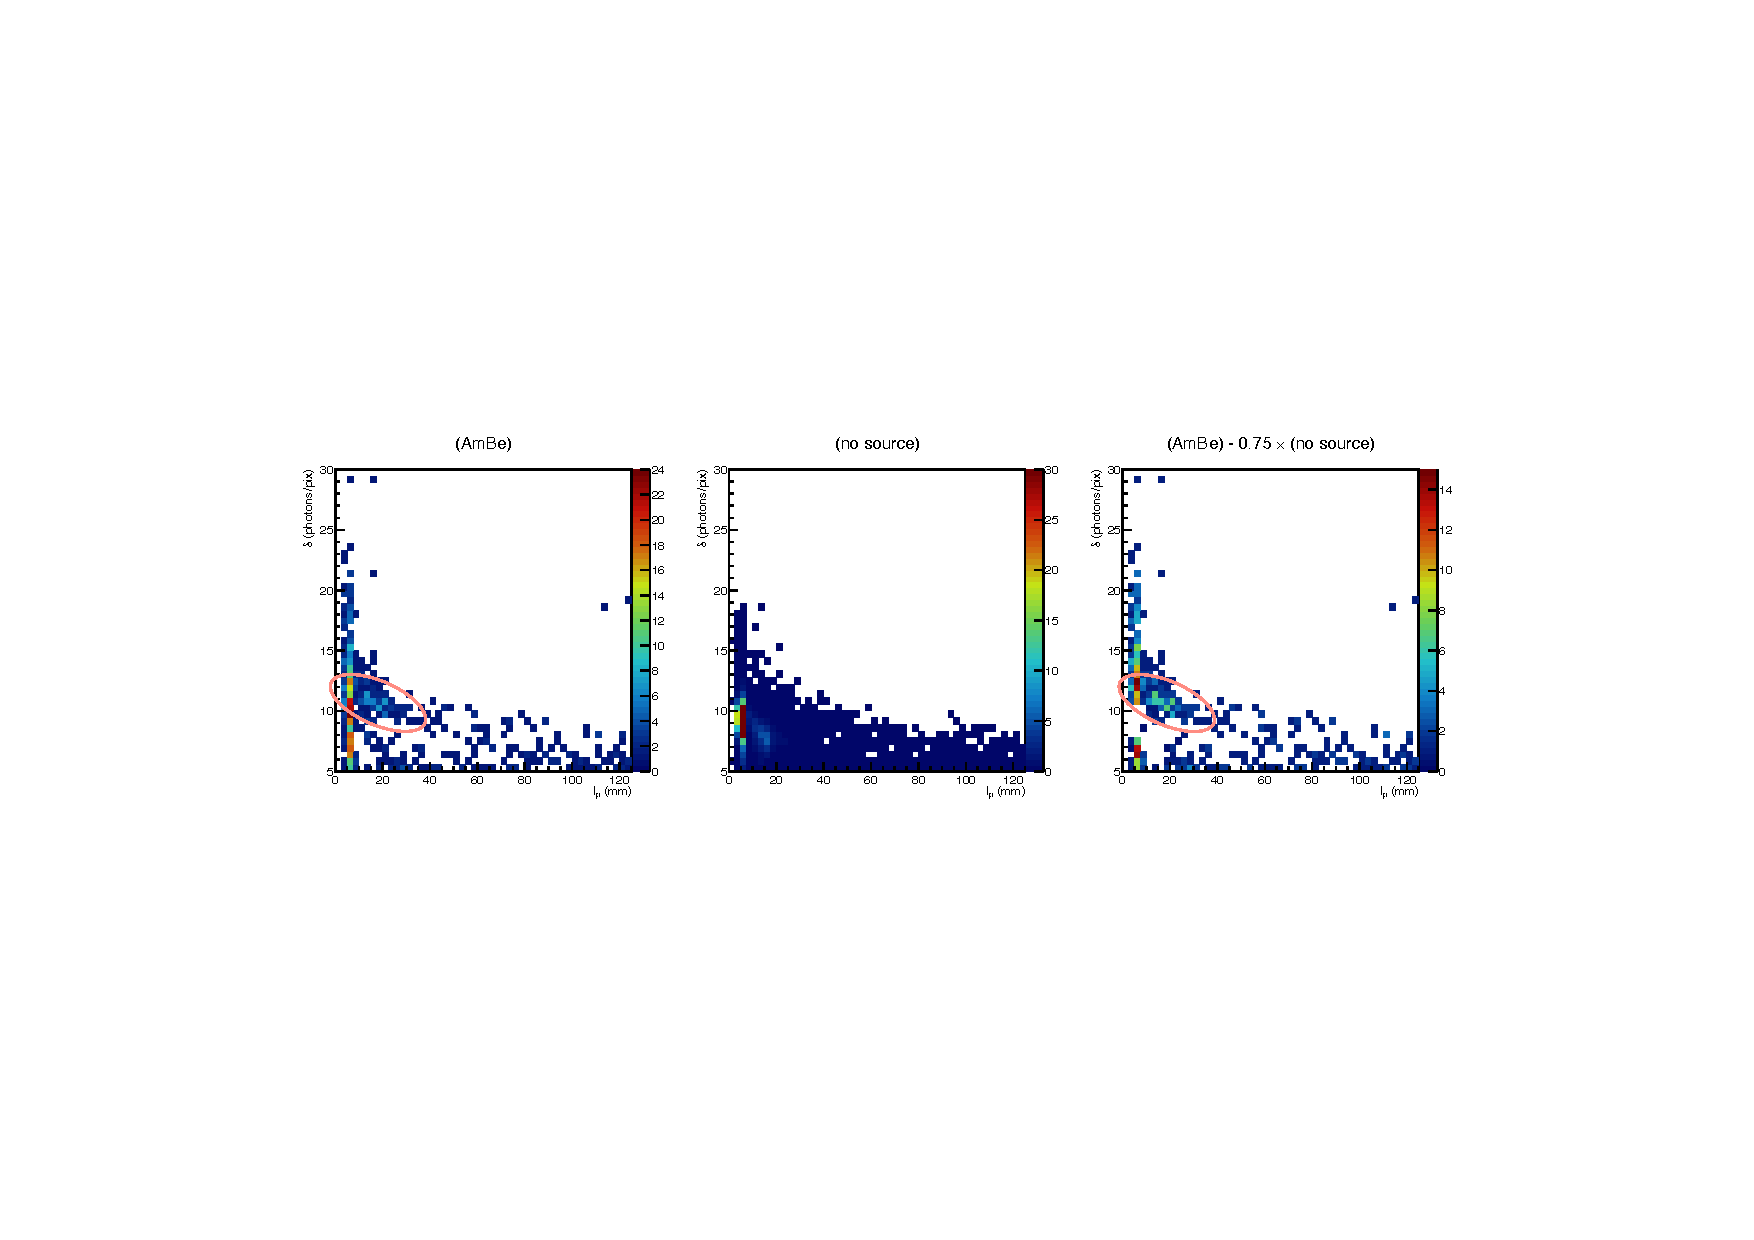
\includegraphics[width=0.90\linewidth]{figures/densityvslength_zoom}

  \caption{Supercluster light density $\delta$ versus length $l_p$,
    for data with \ambe source (left), data without any artificial source
    (middle), and the resulting background-subtracted \ambe data.  The
    normalization of data without source is to the same exposure time
    of the \ambe one, accounting for the trigger scale factor
    $\varepsilon_{SF}$, as defined in the text. \label{fig:dvsl}}

  \end{center}
\end{figure}

\begin{figure}[ht]
  \begin{center}
  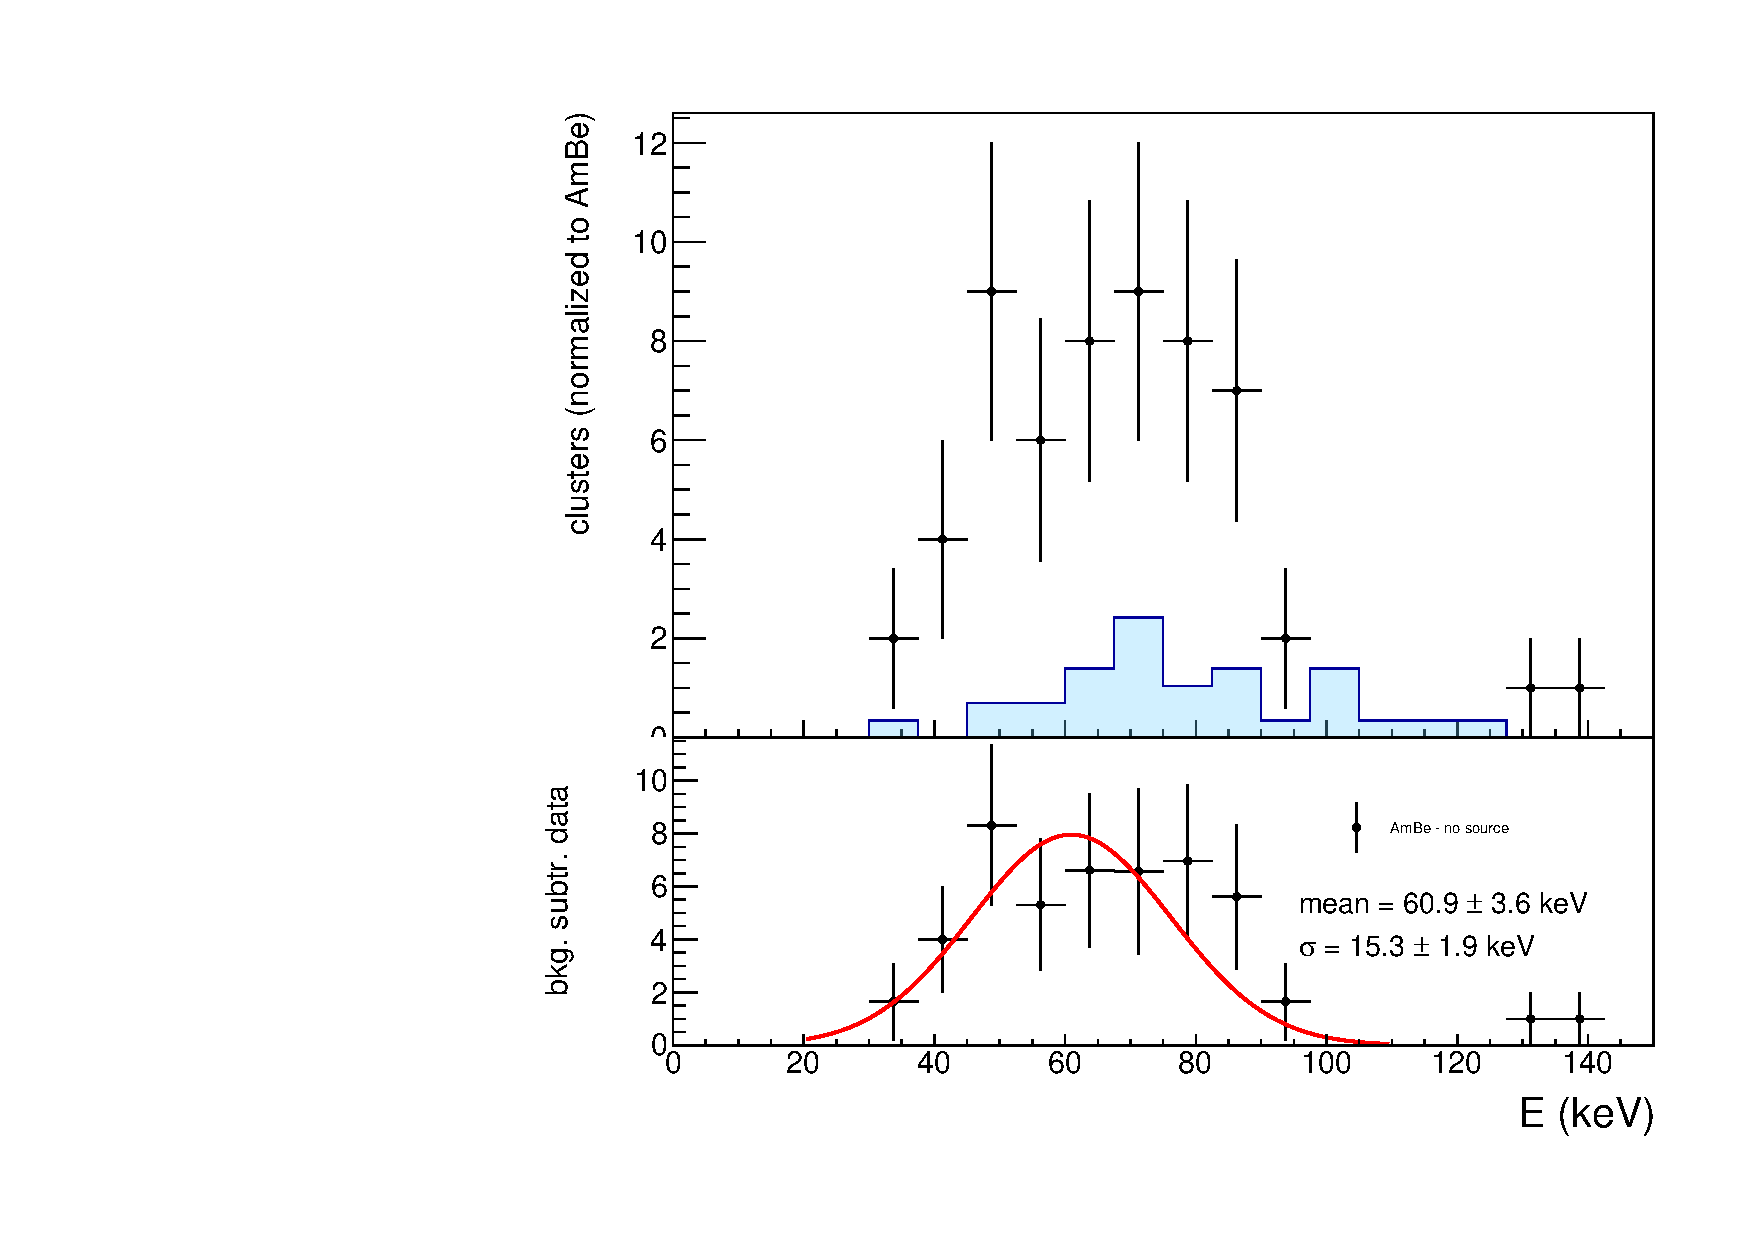
\includegraphics[width=0.60\linewidth]{figures/calintegral_59keV}

  \caption{Calibrated energy spectrum for candidates in the control
    region $PR$, defined in the text. The background-subtracted
    distribution is fitted with a Gaussian PDF, which shows a mean
    value compatible with $E=59\keV$ originated from the $^{241}$Am
    $\gamma$s interaction within the gas. \label{fig:59keV}}

  \end{center}
\end{figure}

\subsection{PMT-based cosmic ray suppression}
An independent information to the light detected by the sCMOS sensor
of the camera is obtained from the PMT pulse, used to trigger the
image shooting. For each image acquired, the corresponding PMT pulse
waveform is recorded.  Tracks from cosmic rays, which typically have a
large angle with respect the cathode plane, as shown in
Fig.~\ref{fig:cosmics} (right), show a broad waveform, characterized
by the different arrival times of the several ionization clusters
produced along the track at different $z$. Conversely, spot-like
signals like \fe deposits or nuclear recoils are characterized by a
short pulse, as shown in Fig.~\ref{fig:waveforms}.
%
\begin{figure}[ht]
  \begin{center}
    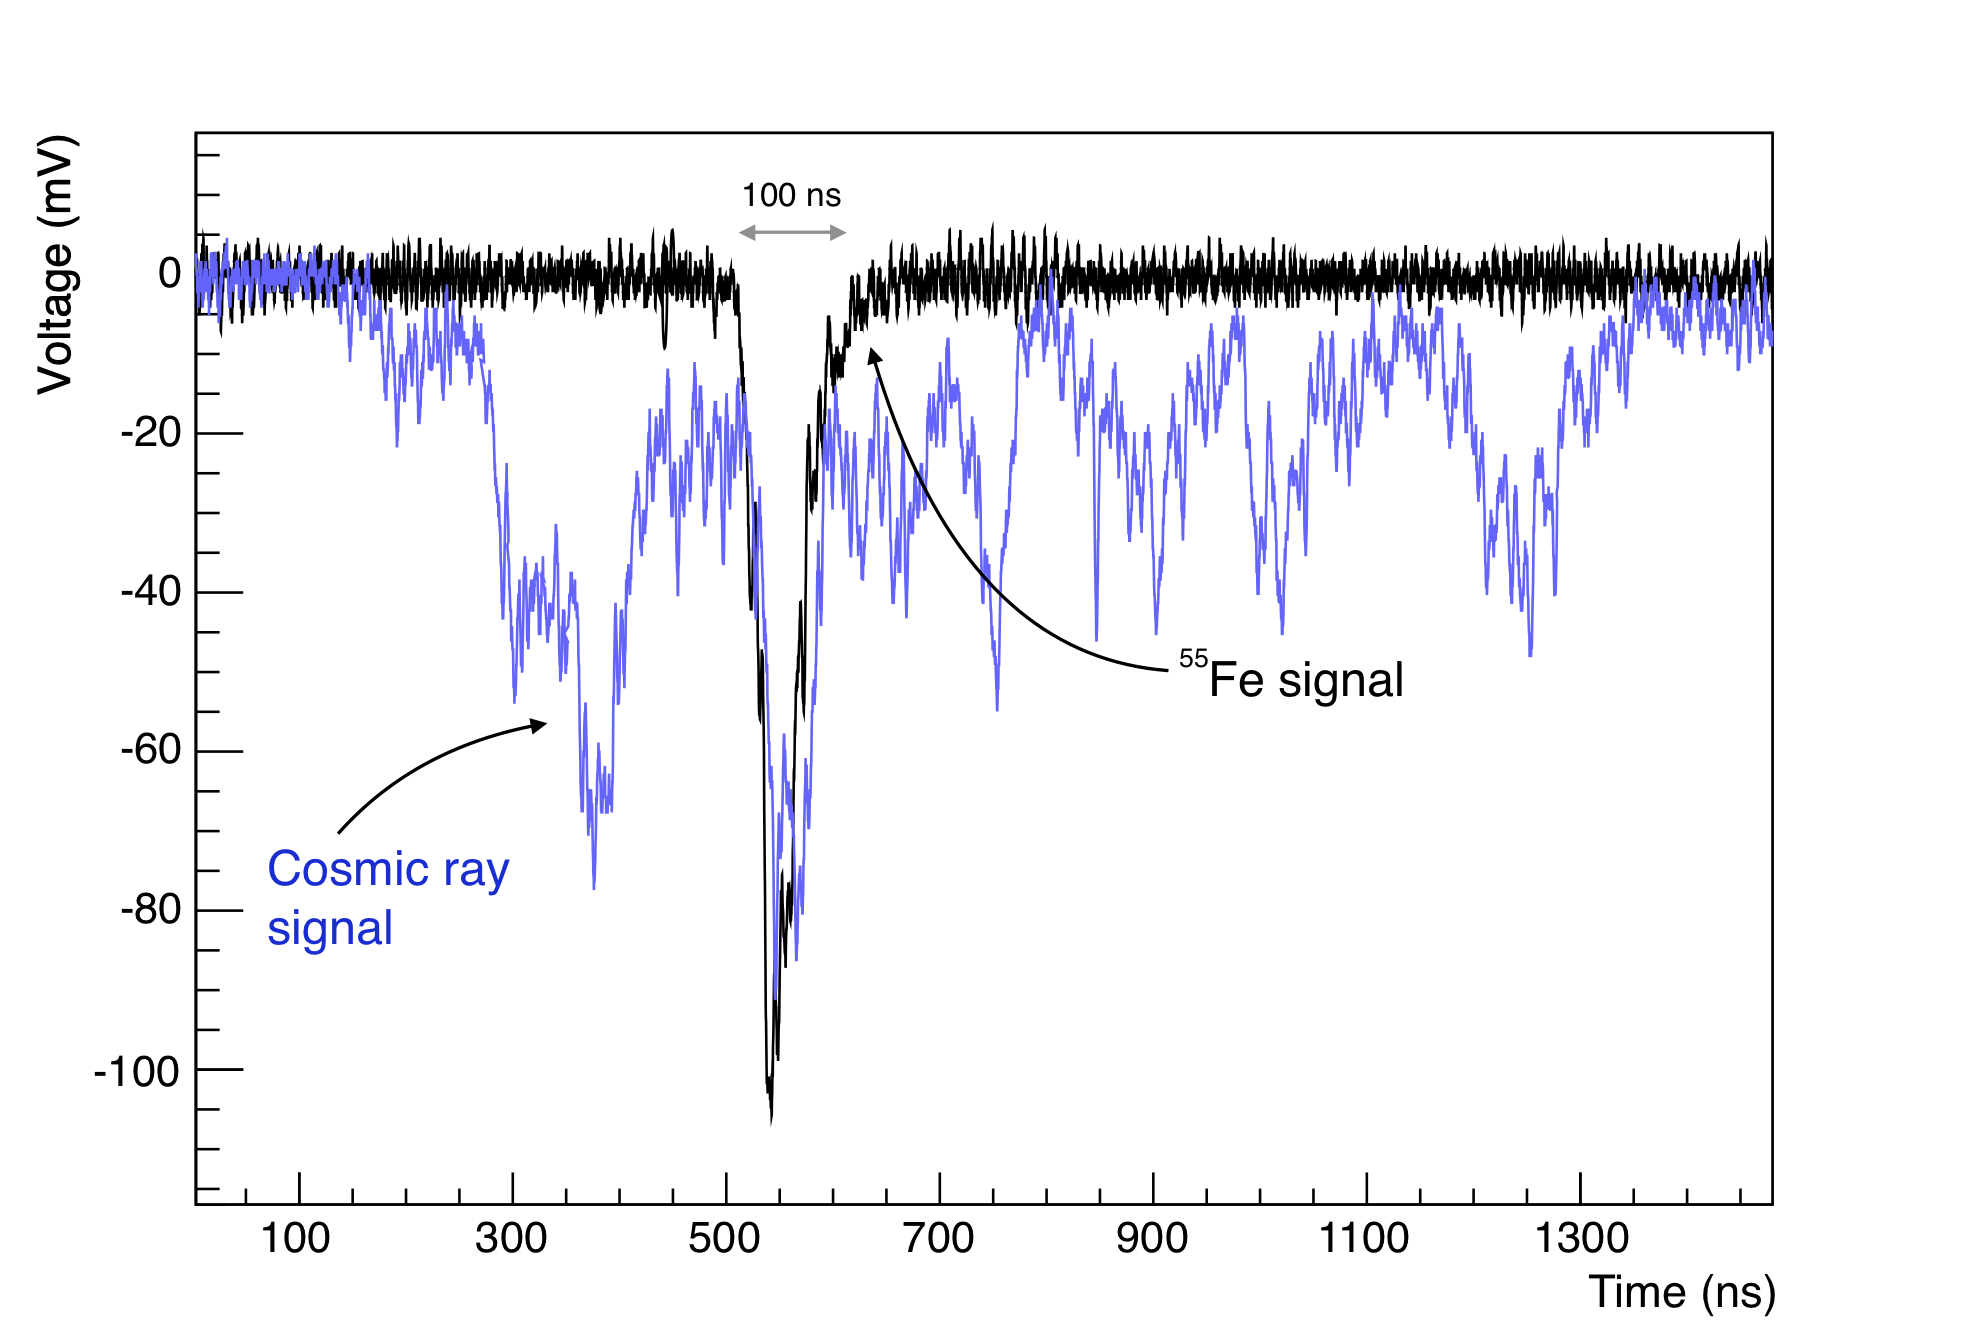
\includegraphics[width=0.69\linewidth]{figures/Waveforms.png}

    \caption{Example of two acquired waveforms: one short pulse
  recorded in presence of \fe radioactive source, together with a long
  signal very likely due to a cosmic ray
  track.  \label{fig:waveforms}}

  \end{center}
\end{figure}

%
The Time Over Threshold (\textit{TOT}) of the PMT pulse was measured,
and is shown in Fig.~\ref{fig:pmttot}. It can be seen from the region
around 270\unit{ns}, dominated by the cosmic rays also in the data
with the \ambe source, that the trigger scale factor
$\varepsilon_{SF}$ also holds for the PMT event rate.
%
\begin{figure}[ht]
  \begin{center}
  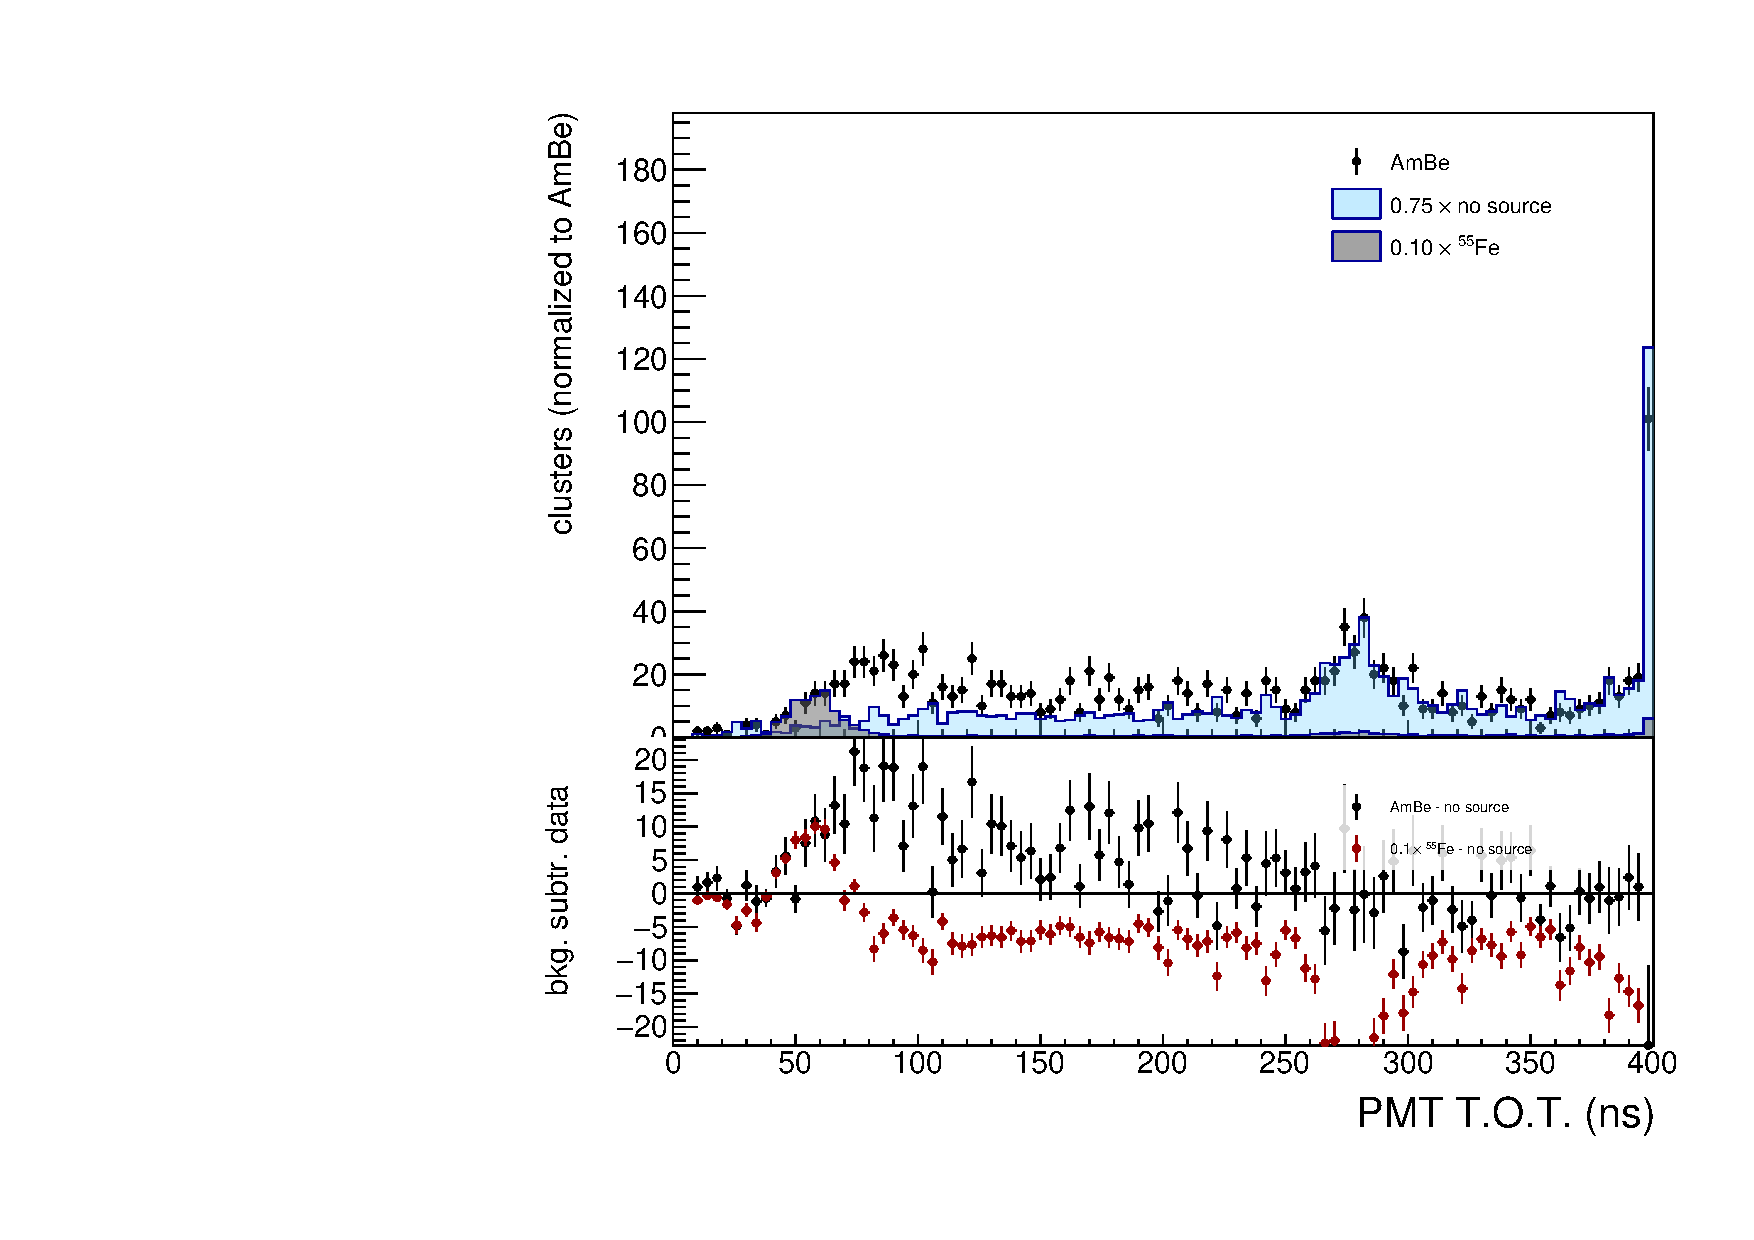
\includegraphics[width=0.45\linewidth]{figures/pmt_tot}

   \caption{PMT waveform time over threshold ($TOT$).  The last bin
    integrates all the events with $TOT>400$\unit{ns}. Filled points
    represent data with \ambe source, dark gray (light blue)
    distribution represents data with \fe source (no source).  The
    normalization of data without source is to the same exposure time
    of the \ambe one, with trigger scale factor $\varepsilon_{SF}$
    applied. For the data with \fe, a scaling factor of one tenth is
    applied for clearness, given the larger activity of this
    source. \label{fig:pmttot}}

  \end{center}
\end{figure}
%
As expected, spot-like clusters (in 3D) correspond to a short pulse in
the PMT, while cosmic ray tracks have a much larger pulse. The
contribution of cosmic ray tracks is clearly visible in the data with
radioactive sources. A selection on this variable is helpful to
further reject residual cosmic rays background present in the \ambe or
\fe data, in particular tracks which may have been split in multiple
superclusters, like the case shown in Fig.~\ref{fig:super_clusters2}
(bottom), and thus passing the above preselection on the cluster
shapes. A selection $TOT<250$\unit{ns} is then imposed.  It has an efficiency of 98\% on cluster candidates in
\ambe data (after background subtraction), while it is only 80\%
efficient on data with \fe source.  The light density, and the energy
spectrum, after the full preselection, is shown in
Fig.~\ref{fig:presel}.
%
\begin{figure}[ht]
  \begin{center}
  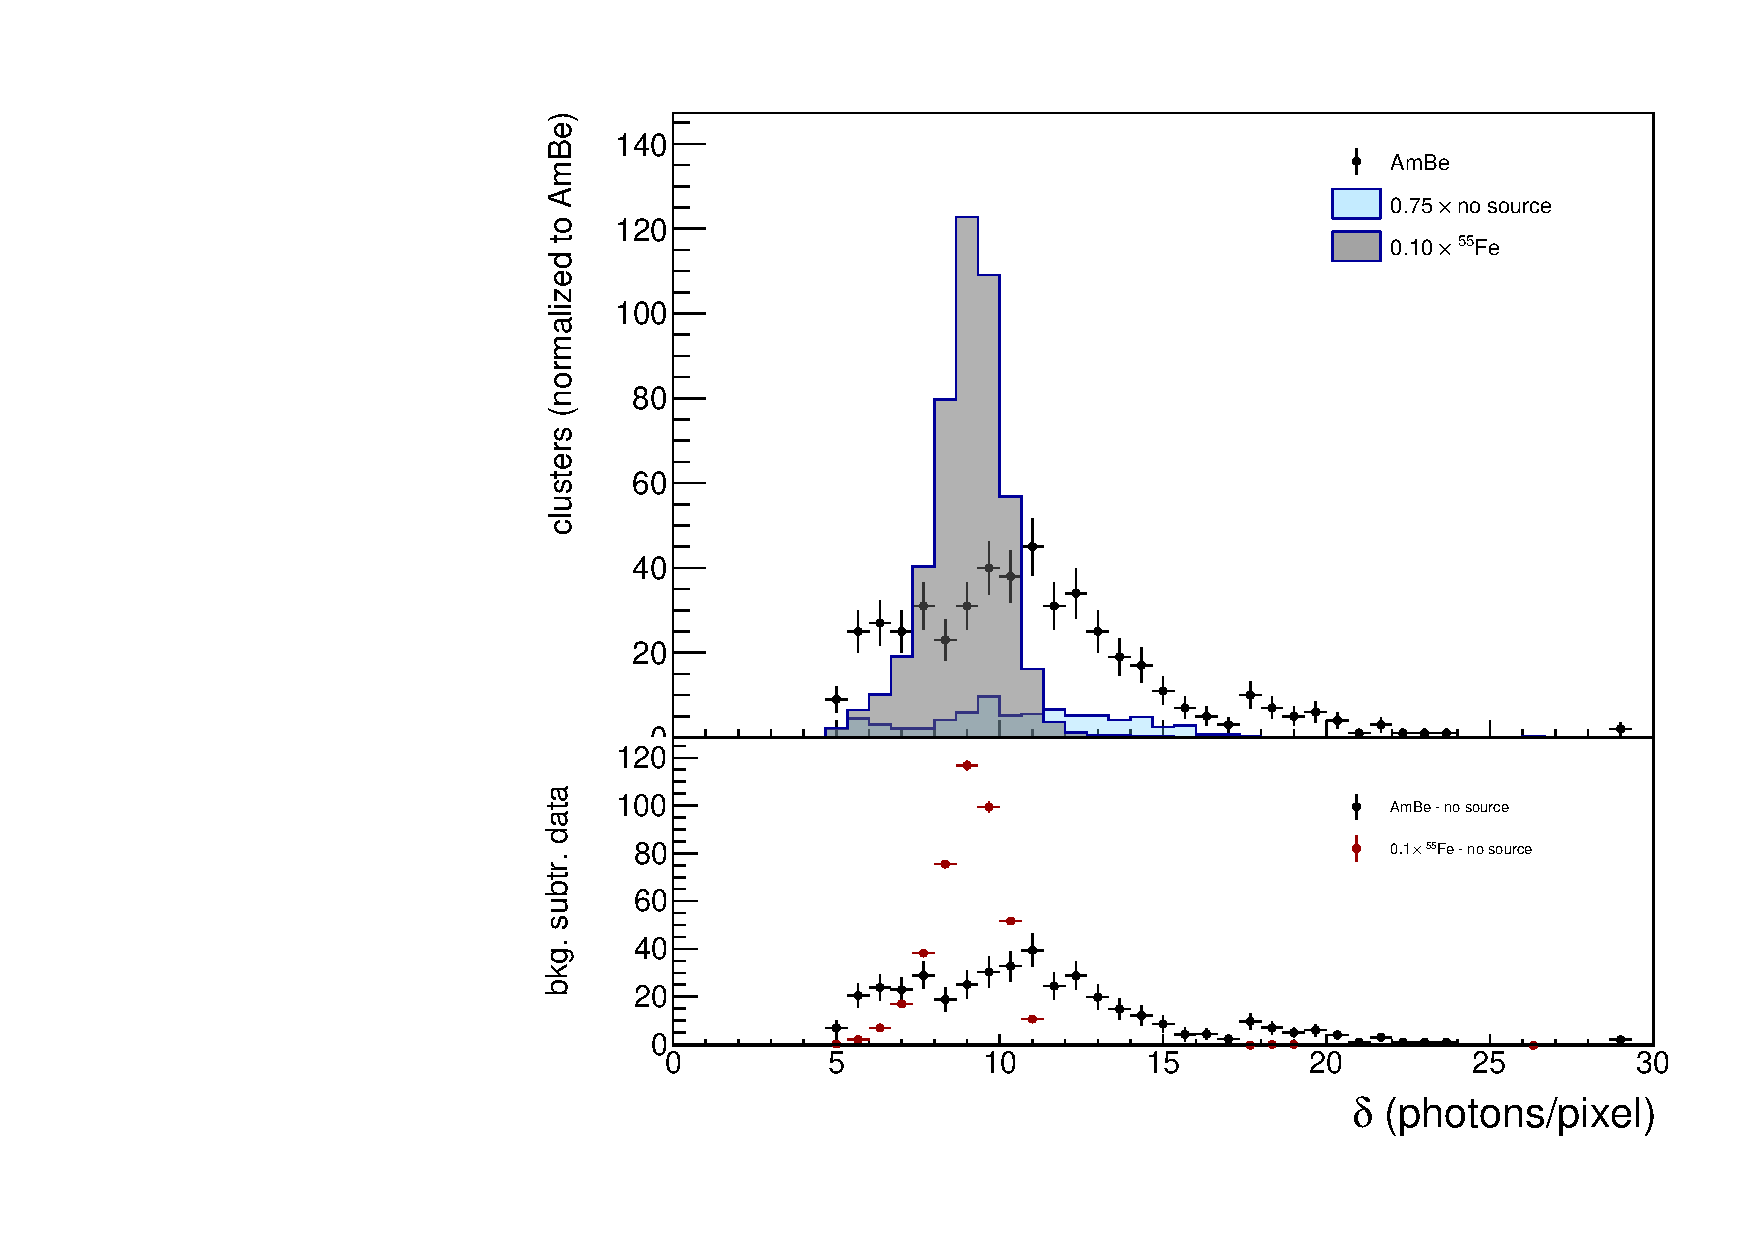
\includegraphics[width=0.45\linewidth]{figures/density_fullSel}
  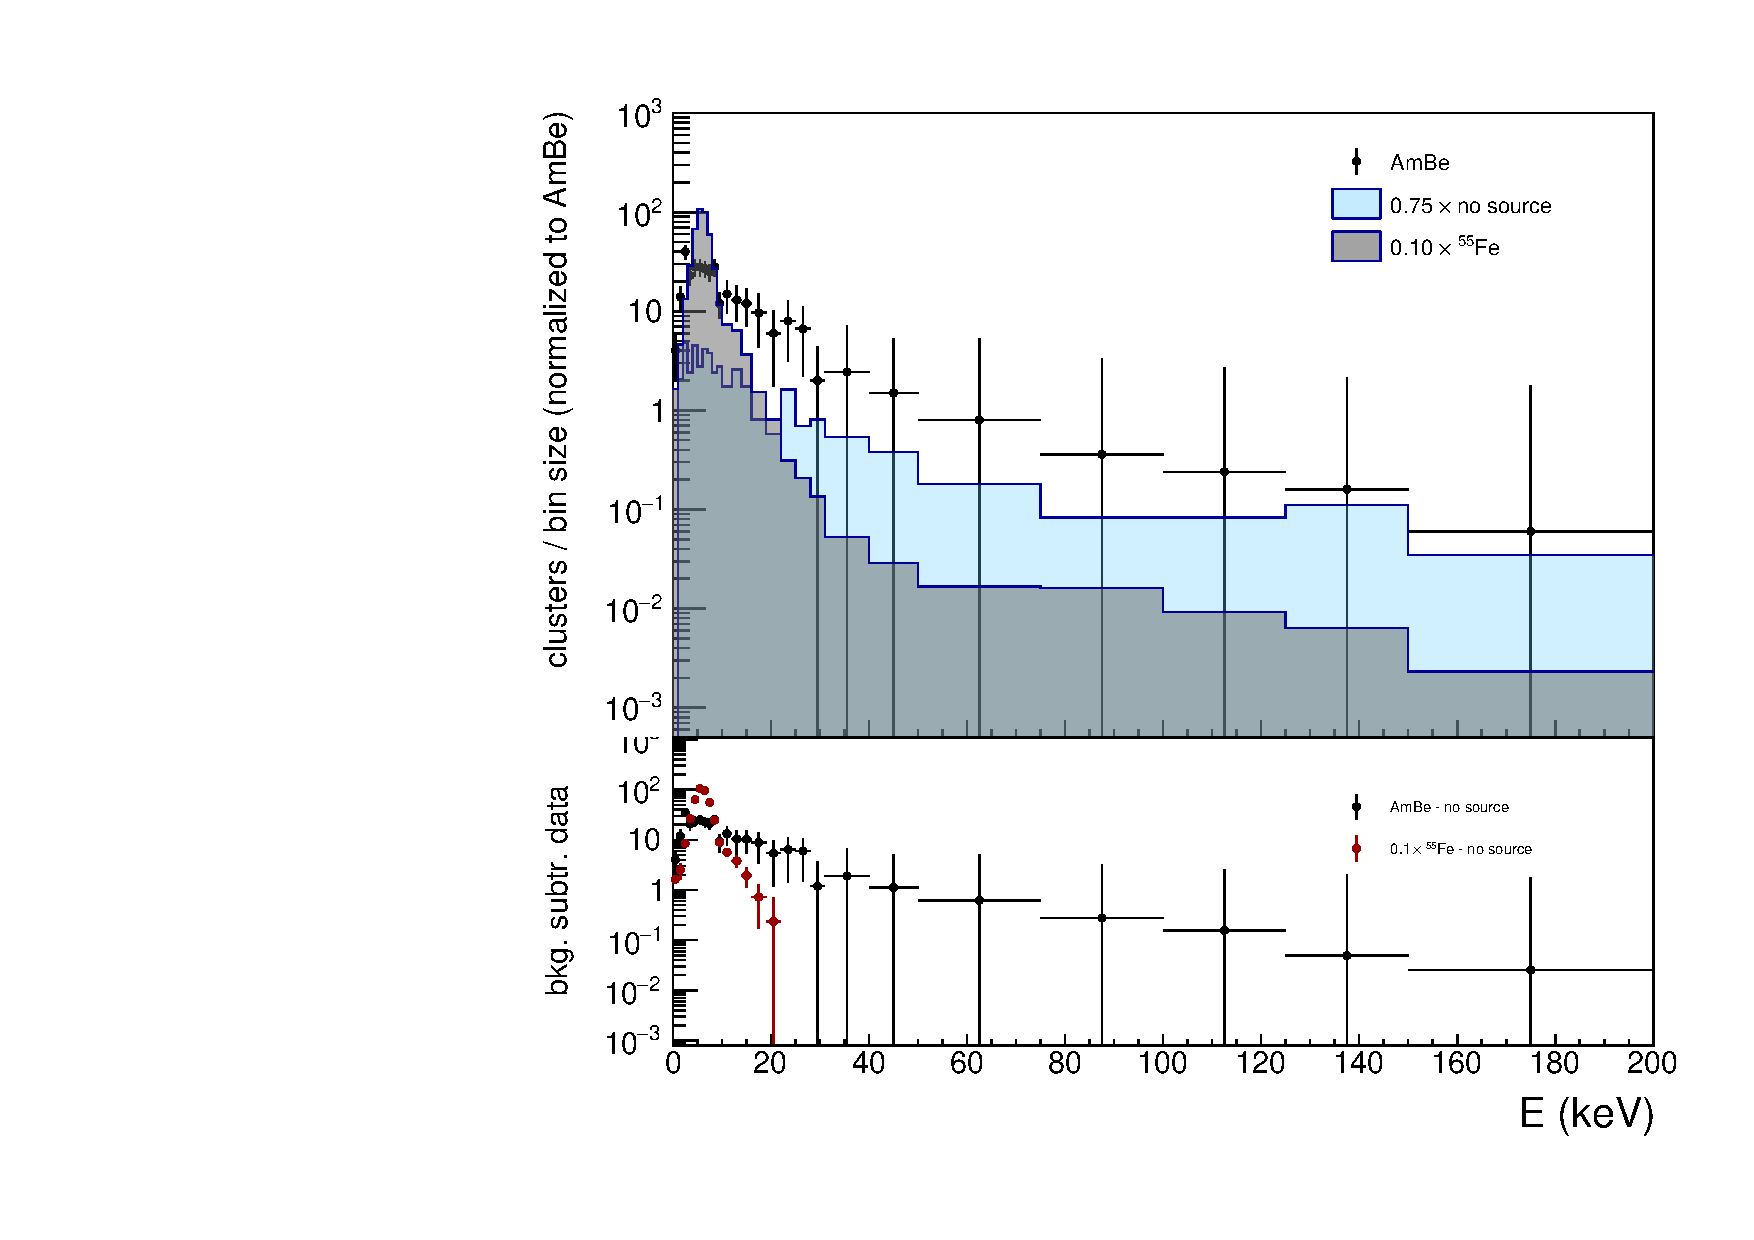
\includegraphics[width=0.45\linewidth]{figures/energy_fullSel}

  \caption{Supercluster light density $\delta$ (left) and calibrated
    energy $E$ (right), after the preselection and cosmic ray
    suppression described in the text to select nuclear recoil
    candidates. Filled points represent data with \ambe source, dark
    gray (light blue) distribution represents data with \fe source
    (no-source).  The normalization of no-source data is to the same
    exposure time of the \ambe data, with the trigger scale factor
    $\varepsilon_{SF}$ applied. For the data with \fe, a scaling
    factor of one tenth is applied for clearness, given the larger
    activity of this source.  \label{fig:presel}}

  \end{center}
\end{figure}

\subsection{Light density and  \fe events rejection}
The light density distribution, after the above preselection and
cosmic ray suppression, appear to be different among the data
with \ambe source, data with \fe source, and data without any
artificial source.  The cosmic-background-subtracted distributions of
$\delta$ in \ambe data and \fe data, shown in the bottom panel of
Fig.~\ref{fig:presel} (left), are used to evaluate a curve of electron
recoils rejection ($1-\varepsilon^\delta_{B}$) as a function of signal
efficiency ($\varepsilon^\delta_{S}$), obtained varying the selection
on $\delta$. This is shown in Fig.~\ref{fig:roc}.  The same procedure
could be applied to estimate the rejection factor against the cosmic
ray induced background, but this is not shown because of the limited
size of the no-source data. This kind of background will however be
negligible when operating the detector underground. This is shown in
Fig.~\ref{fig:roc}. While this cut-based approach is minimalist, and
could be improved by profiting of the correlations among $\delta$ and
the observables used in the preselection in a more sophisticated
multivariate analysis, it shows that a good rejection factor of
electron recoils at $E=5.9\keV$ can be obtained.
%
\begin{figure}[ht]
  \begin{center}
  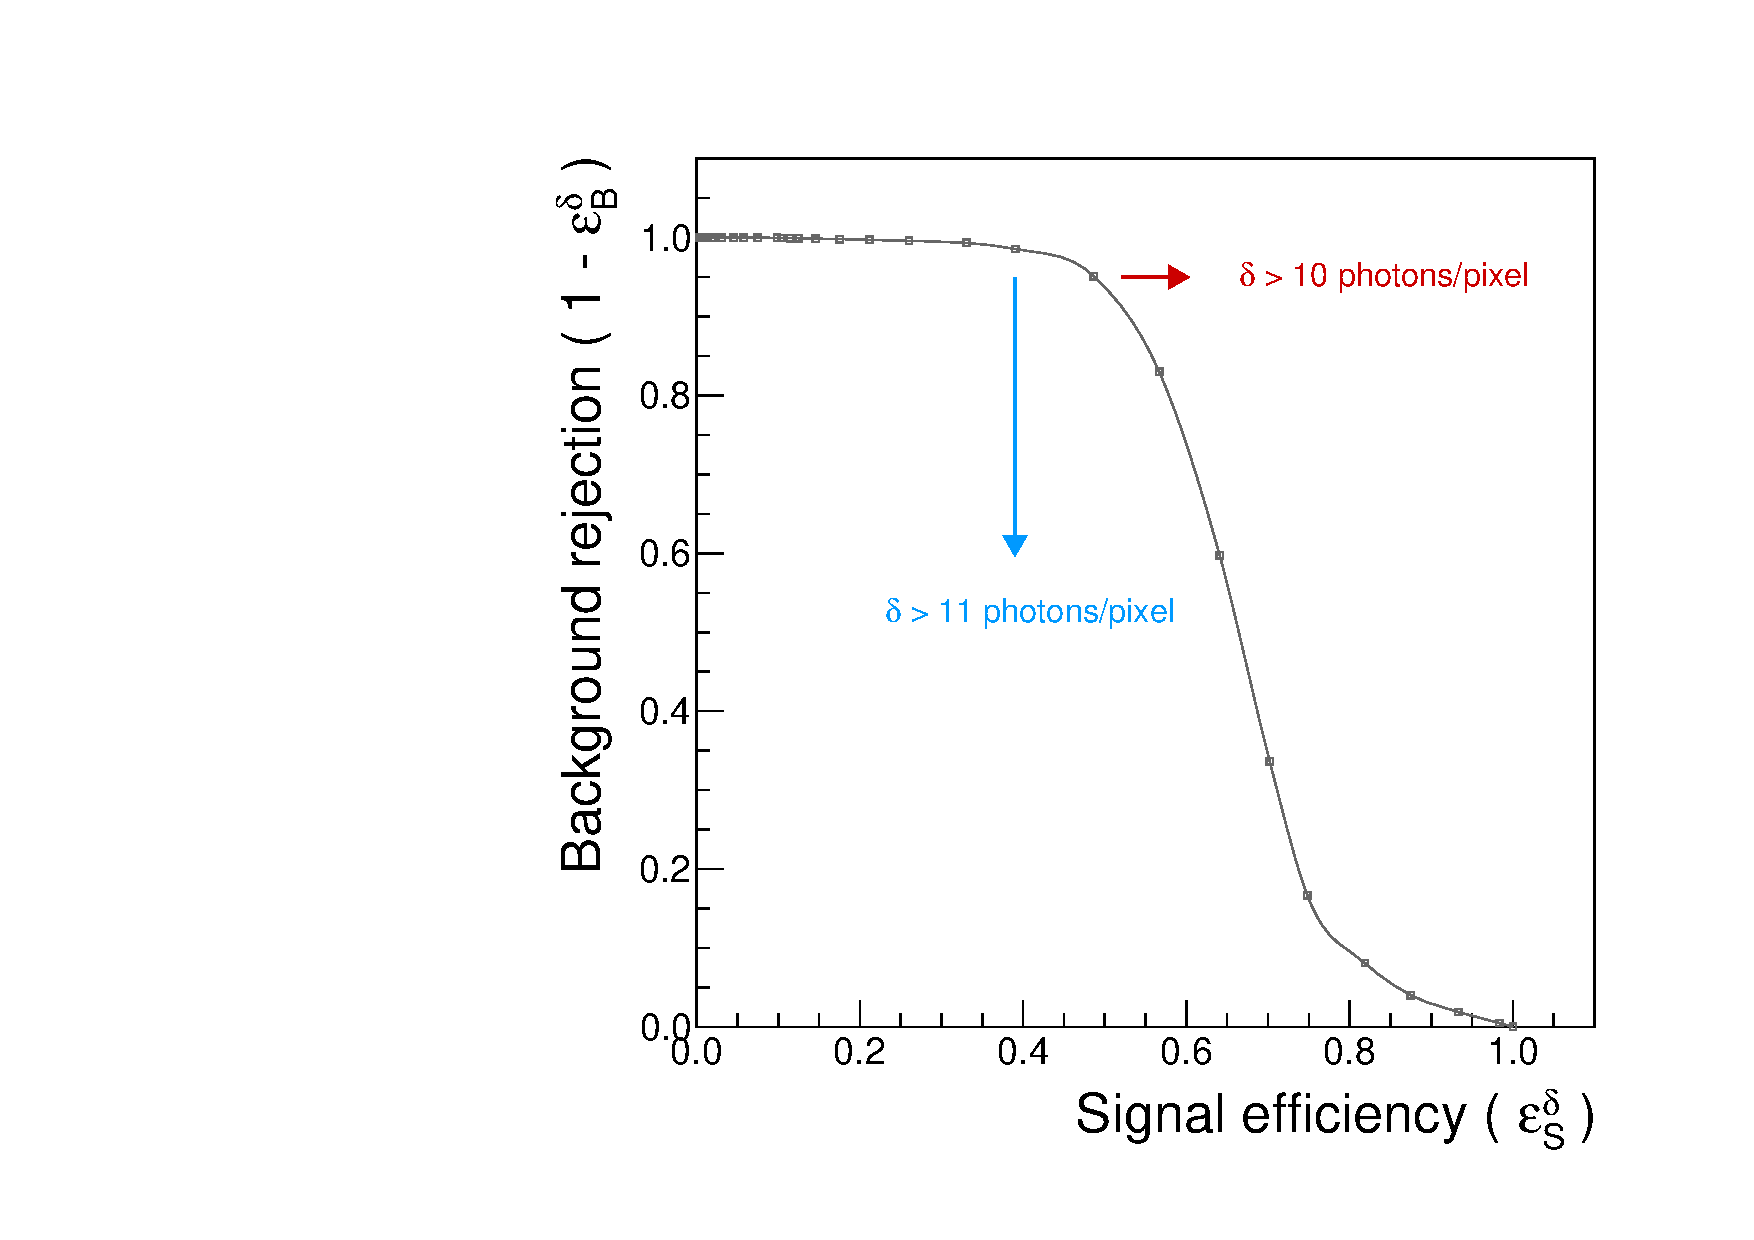
\includegraphics[width=0.45\linewidth]{figures/density_roc}

  \caption{Background rejection as a function of the signal
    efficiency, varying the selection on the $\delta$ variable in data
    with either \fe (background sample) or \ambe (signal sample)
    sources.  \label{fig:roc}}

  \end{center}
\end{figure}
%

 Table~\ref{tab:roc} shows then the
full signal efficiency and electrons rejection factor for two example
working points, $\mathrm{WP}_{40}$ and $\mathrm{WP}_{50}$, having 40\%
and 50\% signal efficiency for the selection on $\delta$. They
correspond to a selection $\delta>11$ and $\delta>10$, respectively.


\begin{table*}[t]
\caption{Signal (nuclear recoils) and background (electron recoils) efficiency for
  two different selections on $\delta$.\label{tab:roc}}
\vspace{10pt}
\normalsize
\centering
\begin{tabular}{l c c c | c c c }
  \hline\hline
  working point & \multicolumn{3}{c}{Signal efficiency} & \multicolumn{3}{c}{Background efficiency} \\
  \hline
  & $\varepsilon_{S}^{presel}$ & $\varepsilon_{S}^{\delta}$ & $\varepsilon_{S}^{total}$ & $\varepsilon_{B}^{presel}$ & $\varepsilon_{B}^{\delta}$ & $\varepsilon_{B}^{total}$ \\
  \hline
  $\mathrm{WP}_{50}$  & 0.98                        & 0.51                      & 0.50                     & 0.70                     & 0.050                     & 0.035 \\
  $\mathrm{WP}_{40}$  & 0.98                        & 0.41                      & 0.40                     & 0.70                     & 0.012                     & 0.008 \\
  \hline\hline
\end{tabular}
\end{table*}

\subsection{Signal Energy Spectrum and efficiency}
The energy spectrum for the candidates with $\varepsilon_{S}^{total}$
= 50\% in the \ambe sample is shown in Fig.~\ref{fig:fullsel_effi}
(left). With the full $\mathrm{WP}_{50}$ selection, the signal
efficiency is computed for both the example working points in bins of
energy. The electron recoil efficiency, $\varepsilon_{B}^{total}$,
represents a $\gamma$ background efficiency at a fixed energy
$E=6\keV$, that is close to the \fe emitted photon energy. For the
$\mathrm{WP}_{50}$, the efficiency for very low-energy recoils,
$E=6\keV$, is still 18\%, dropping to almost zero at $E\lesssim4\keV$.

\begin{figure}[ht]
  \begin{center}
    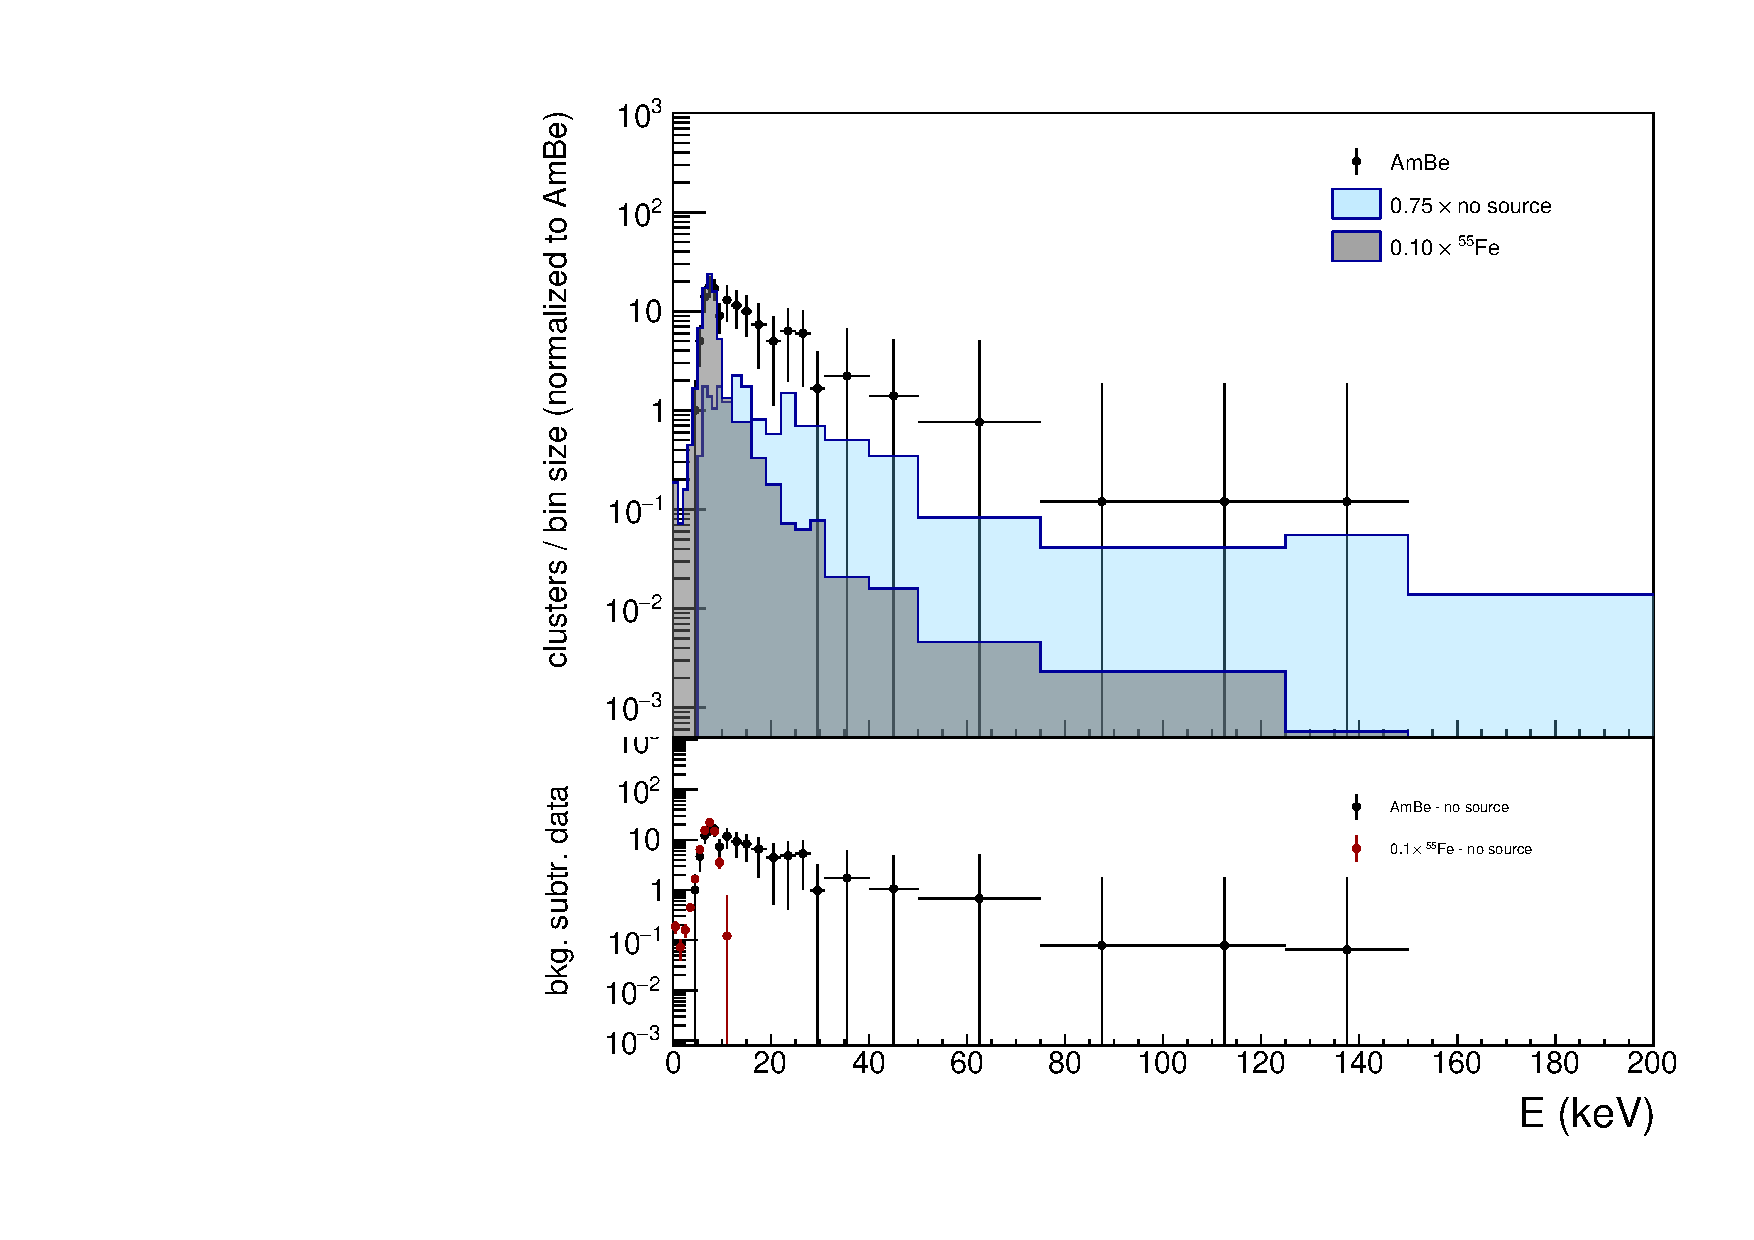
\includegraphics[width=0.45\linewidth]{figures/energyFull_WP50}
    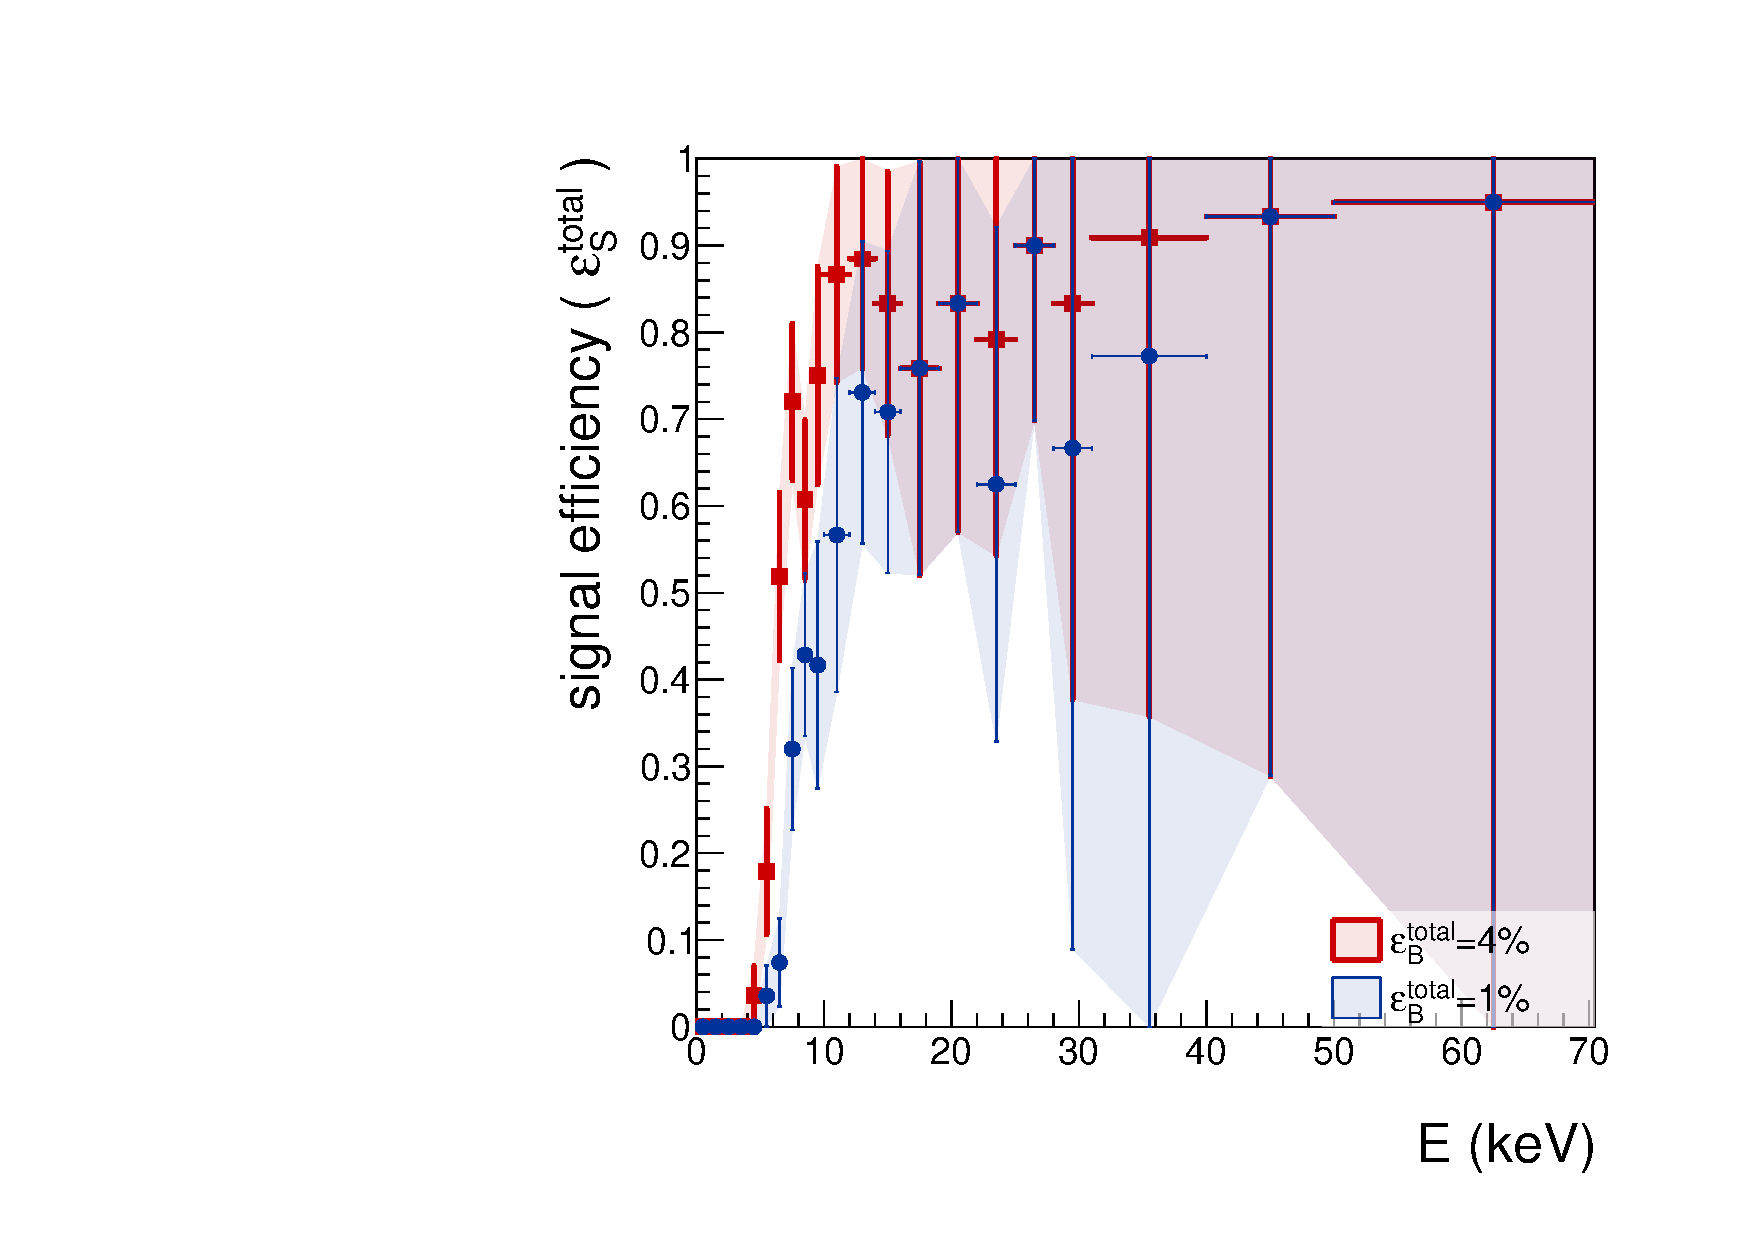
\includegraphics[width=0.45\linewidth]{figures/energyFull_effi}

    \caption{Left: supercluster calibrated energy $E$ (left), after the
      full selection, which includes $\delta>10$, 50\% efficient on
      signal, to select nuclear recoil candidates. Filled points
      represent data with \ambe source, dark gray (light blue)
      distribution represents   \fe source (no-source) data.  The
      normalization of no-source  data  is to the same exposure
      time of the \ambe data, with the trigger scale factor
      $\varepsilon_{SF}$ applied. For the  \fe data, a scaling
      factor of one tenth is applied for clearness, given the larger
      activity of this source. Right: efficiency for nuclear recoil
      candidates as a function of energy, estimated on \ambe data, for
      two example selections, described in the text, having either 4\%
      or 1\% efficiency on electron recoils at
      $E=6\keV$. \label{fig:fullsel_effi}}

  \end{center}
\end{figure}

Two candidate  nuclear recoils images, fulfilling the 
$\mathrm{WP}_{50}$ selection  (with a light density $\delta\gtrsim10$
photons/pixels and with energies of 5.2 and 6.0\keV)  are shown in
Fig.~\ref{fig:lowEnergyNR}. The displayed images are a portion of the full-resolution frame, after the pedestal subtraction.

\begin{figure}[ht]
  \begin{center}
  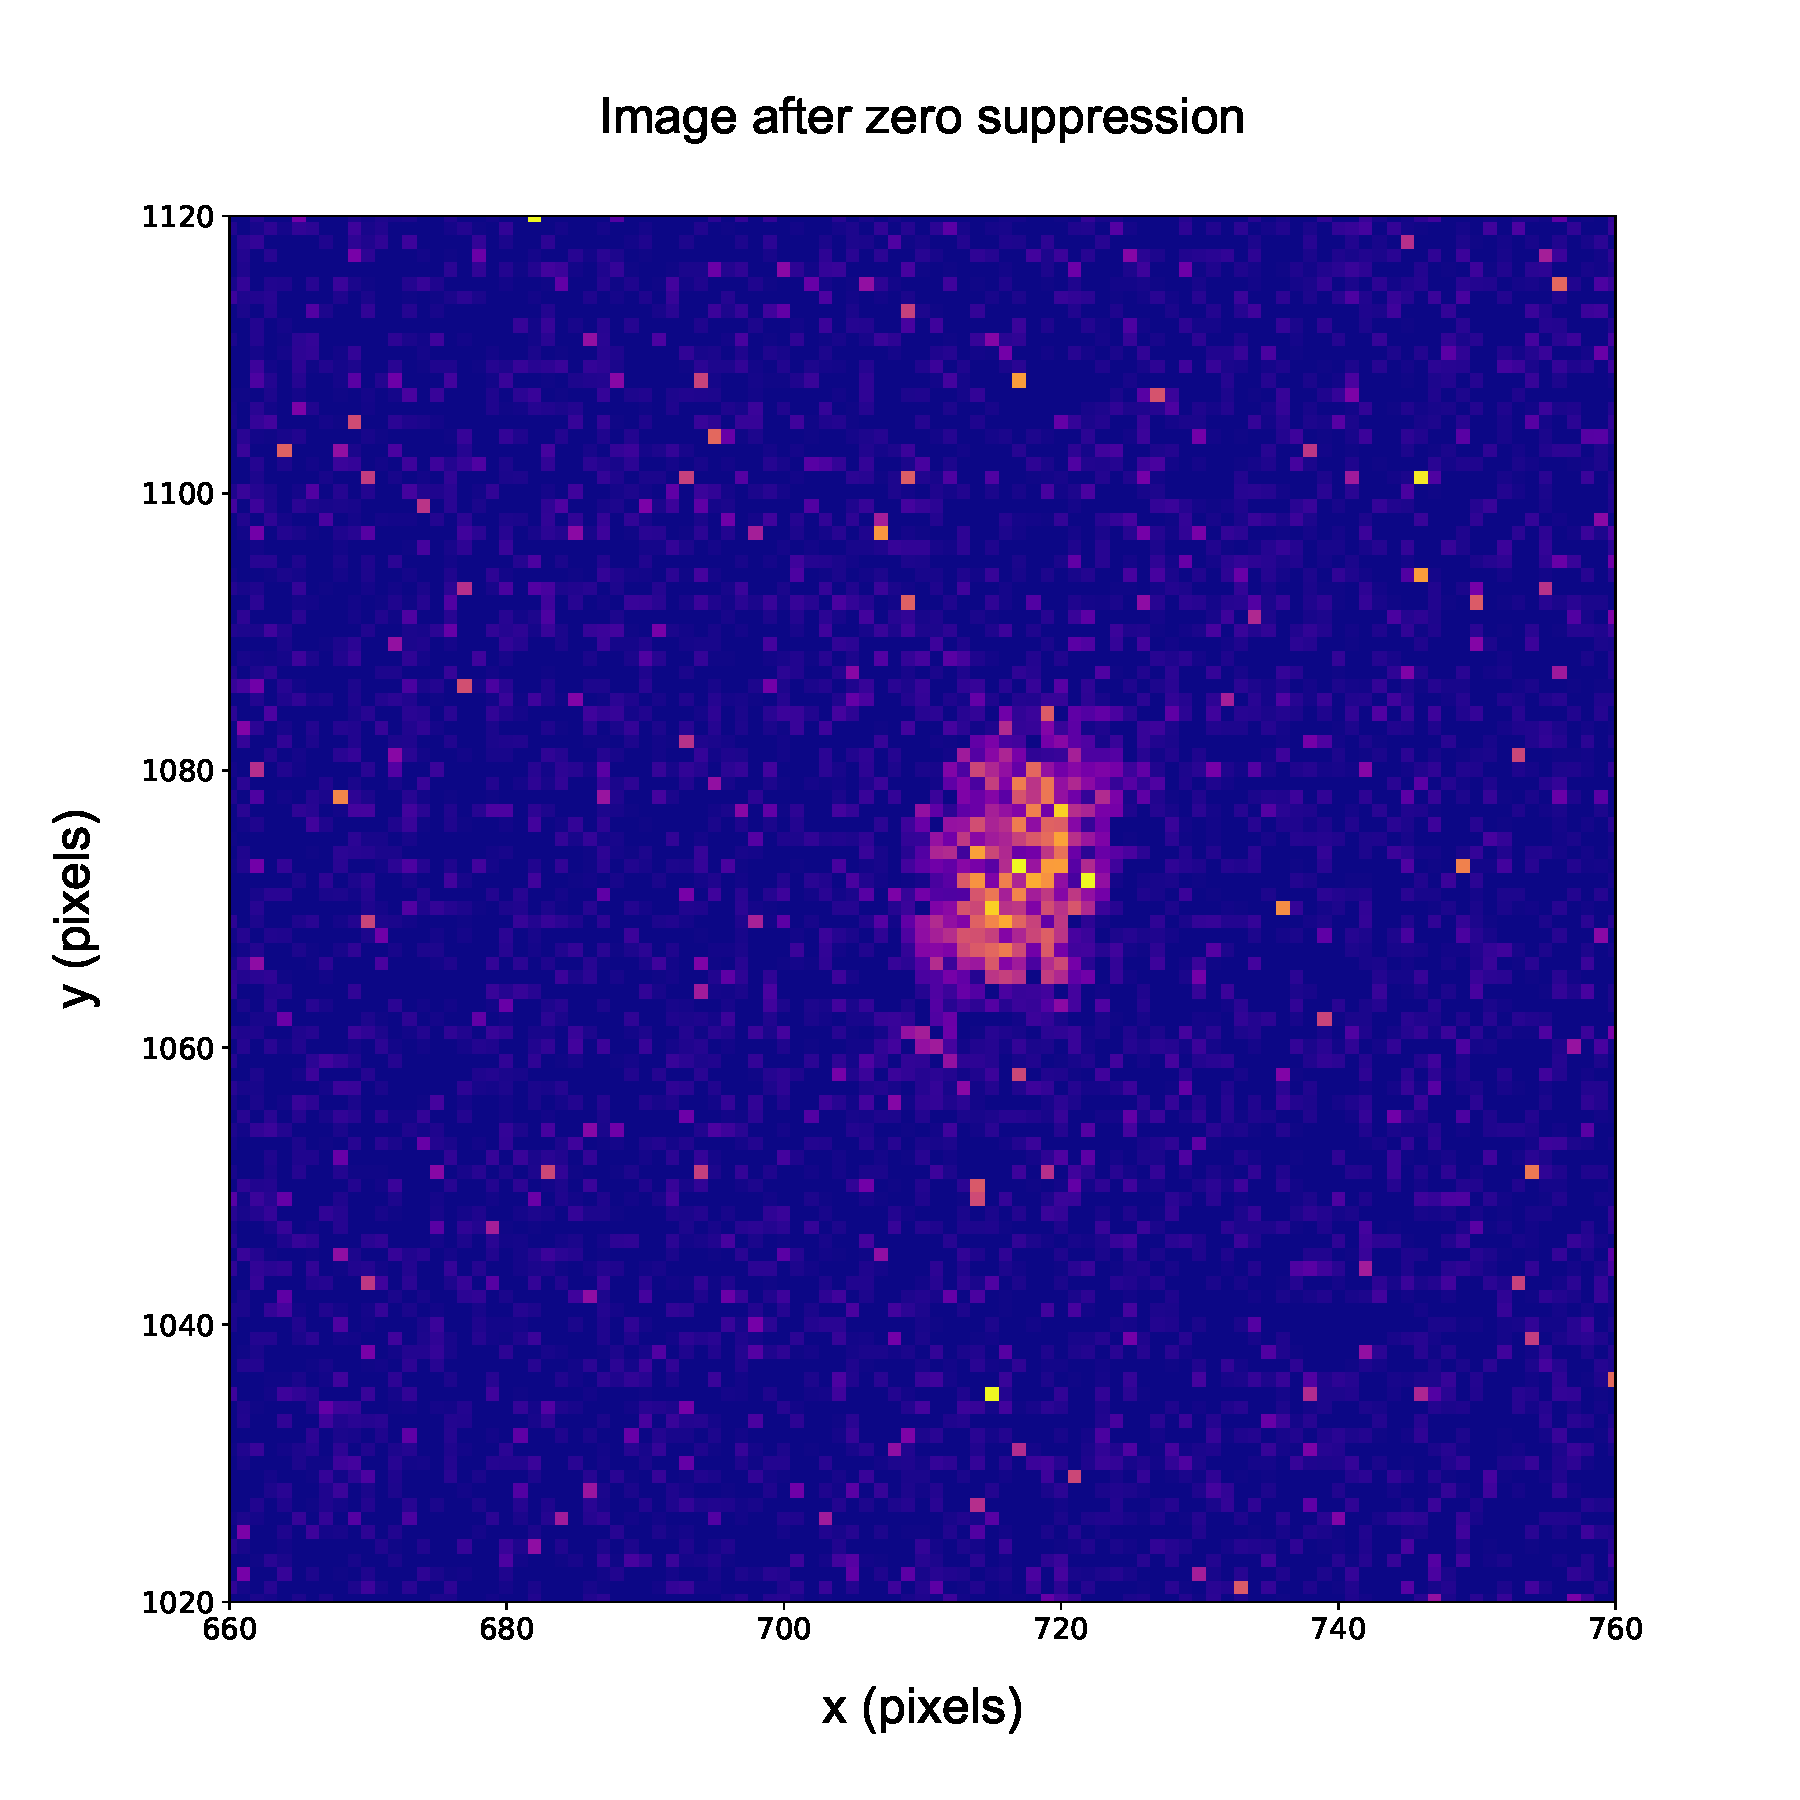
\includegraphics[width=0.49\linewidth]{figures/pic_run02097_ev59_oriIma_paper}
  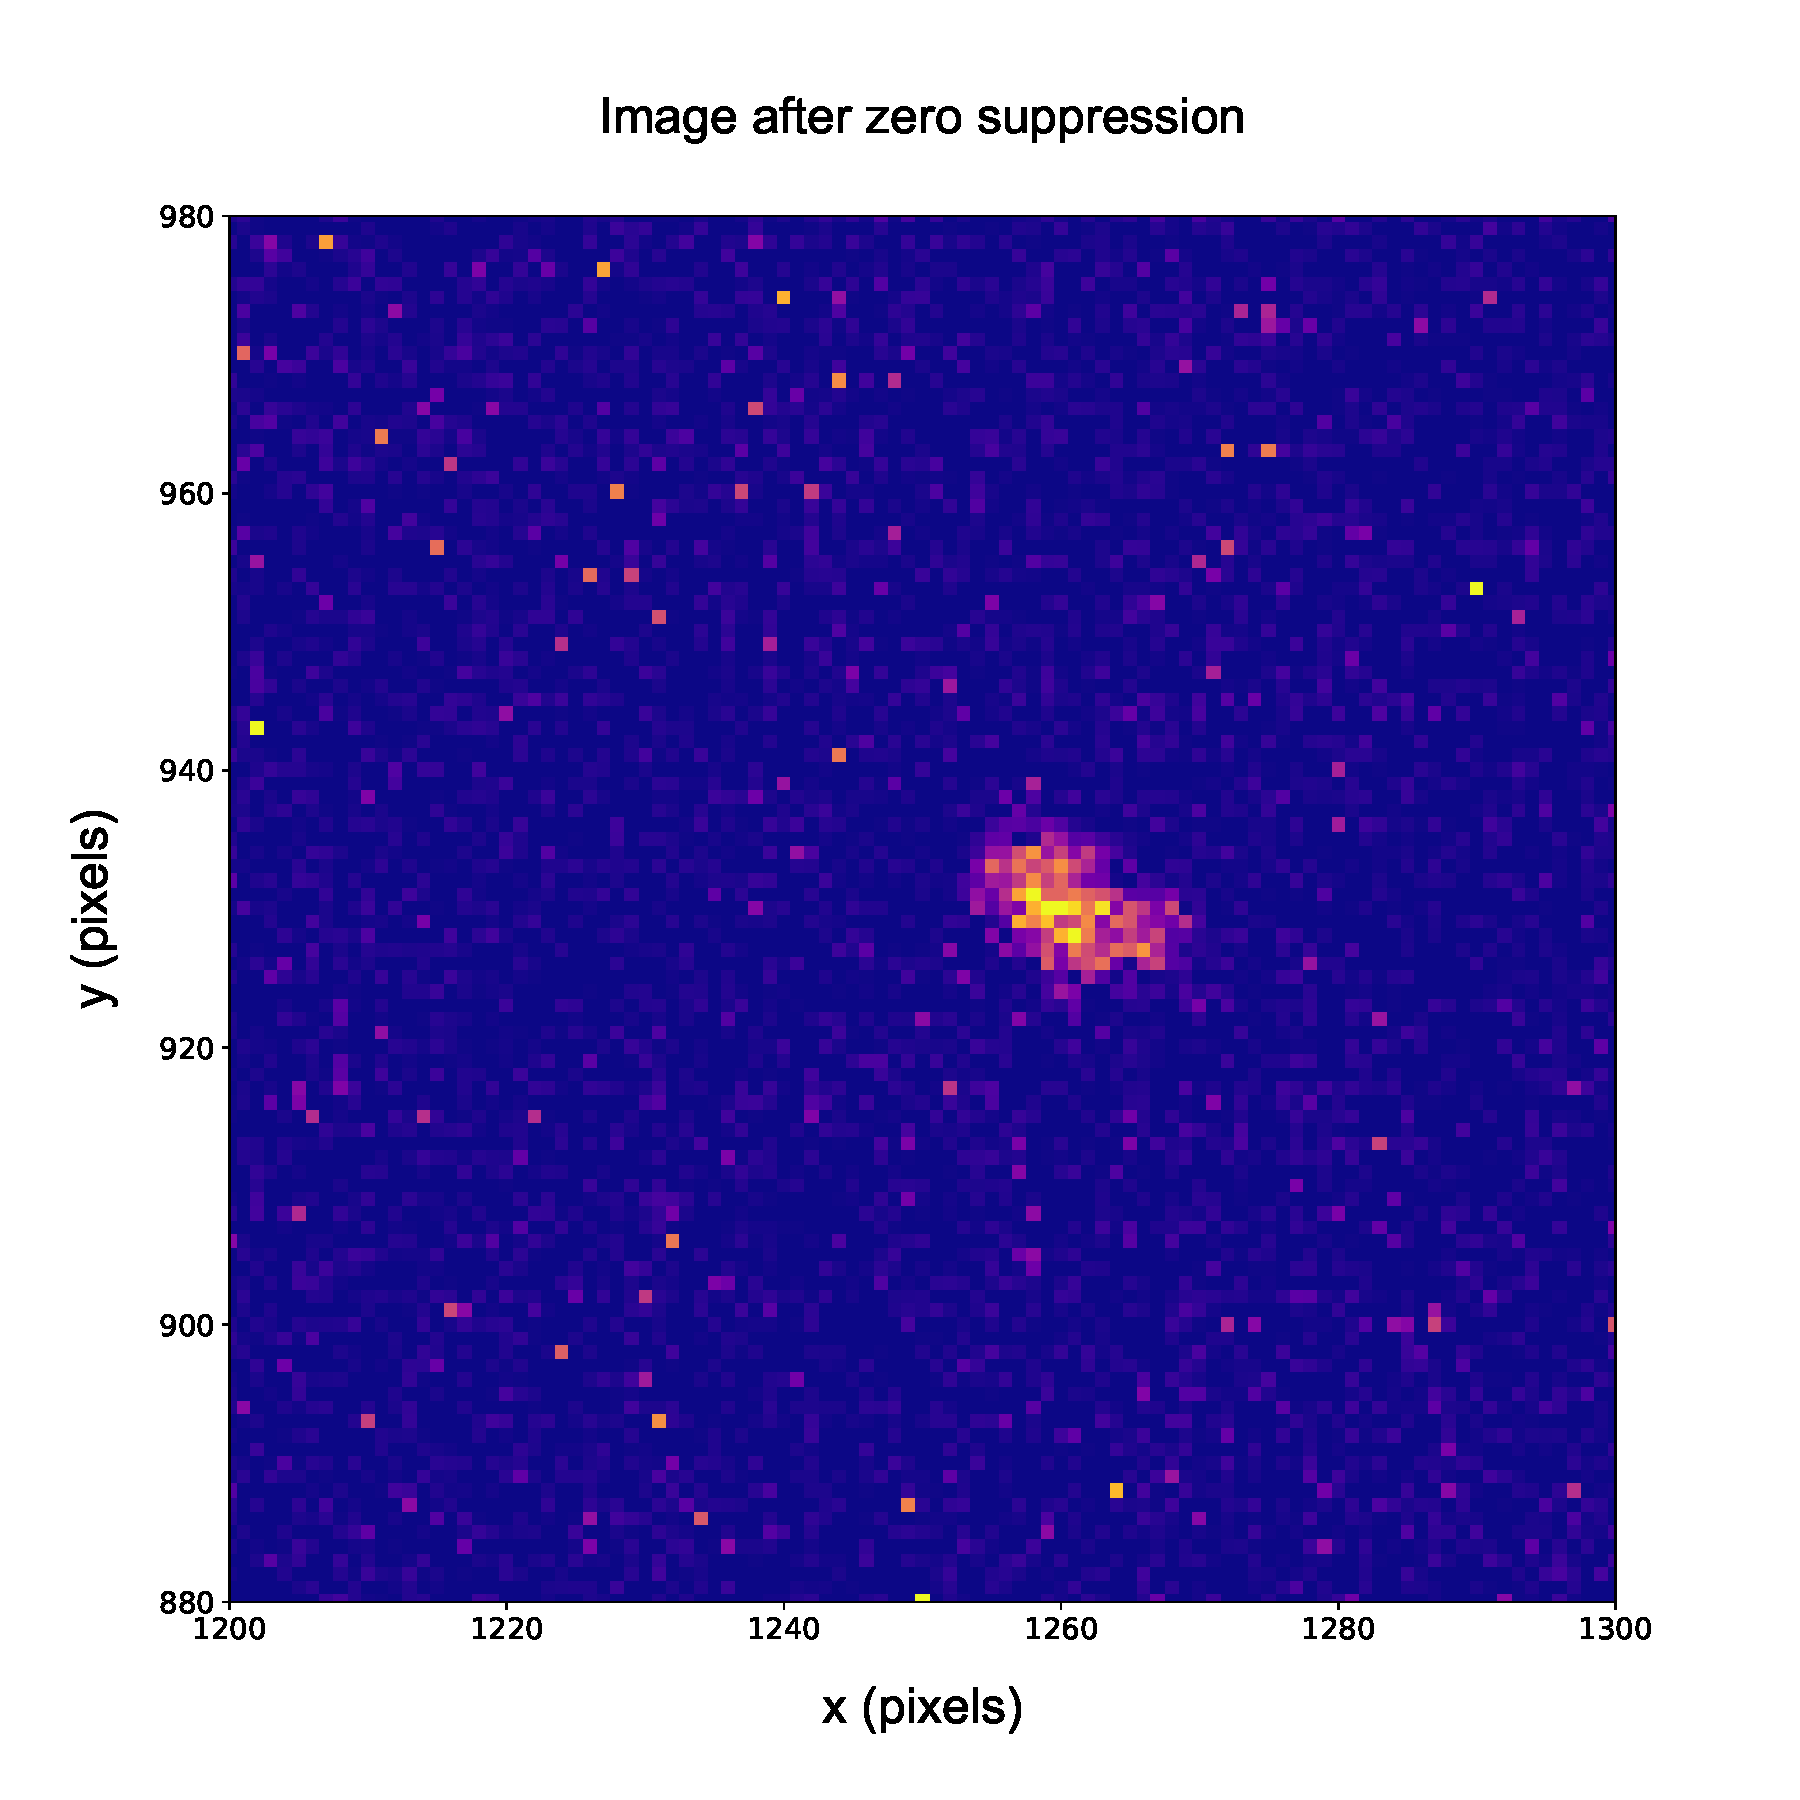
\includegraphics[width=0.49\linewidth]{figures/pic_run02097_ev317_oriIma_paper}

  \caption{Examples of two nuclear recoil candidates, selected with  the full selection, shown in a portion of $100\times100$ pixel matrix, after the zero suppression of the image. Left: a candidate
    with $E=5.2\keV$ and $\delta=10.5$, right: a candidate with
    $E=6.0\keV$ and $\delta=10$.  \label{fig:lowEnergyNR}}

\end{center}
\end{figure}


 
\clearpage


 \section{Conclusion and outlook}

A method to efficiently identify recoiling nuclei after an elastic
scattering with fast neutrons with an optically readout TPC was
presented in this paper.  A 7 liter prototype was employed by exposing
its sensitive volume to two kinds of neutral particles in an
overground location:
\begin{itemize}
\item photons with energy of 5.9~\keV and 59~\keV respectively
  provided by a radioactive source of \fe and by one of $^{241}$Am
  able to produce electron recoils with equal energy by means of
  photoelectric effect;
\item neutrons with kinetic energy of few MeV produced by an \ambe
  source that can create nuclear recoils with kinetic energy lower
  than the neutron ones.
\end{itemize}

The high sensitivity of the adopted sCMOS optical sensor allowed a
very good efficiency in detecting events with an energy released in
gas even below 10~\keV.

Moreover, the possibility of exploiting the topological information
(shape, size and more) of clusters of emitted light permitted to
develop algorithms able to reconstruct not only the total released
energy, but also to identify the kind of the recoiling ionizing
particles in the gas (either an electron or a nucleus). Cosmic ray
long tracks are also clearly separated.

Because of their larger mass and electric charge, nuclear recoils are
expected to release their energy by ionizing the gas molecules in few
hundreds \unit{$\mu$m} while the electrons are able to travel longer
paths. For this reason, by exploiting the spatial distribution of the
collected light, it was possible to identify 5.9\keV electron recoils
with an efficiency of 96.5\% (99.2\%) against nuclear recoils by
retaining a capability of detecting them with an efficiency of 50\%
(40\%), averaged across the measured \ambe spectrum.

In average, nuclear recoils with a kinetic energy lower than 10\keV
can be detected with an efficiency of about 14\%.

The results obtained in the studies presented in this paper can be
improved by means of more sophisticated analyses exploiting a
multivariate approach, which combines a more complete topological
information about the light distribution along the tracks.  Additional
enhancement of sensitivity can be achieved with a DAQ system
collecting single PMT waveforms to be correlated with the track
reconstructed in the sCMOS images.

\section{Acknoledgements}
We are grateful to Servizio Sorgente LNF...  This work was supported
by the European Research Council (ERC) under the European Union’s
Horizon 2020 research and innovation program (grant agreement No
818744)”.

\bibliographystyle{ieeetr}
\bibliography{LEMON-20-001}


\end{document}

